\documentclass[main.tex]{subfiles}
\begin{document}

\newtheorem{defFr}{Définition}
\newtheorem{regleem}{Règle}
\newtheorem{exemple}{Exemple}
\renewcommand{\tablename}{Tableau}
\renewcommand{\chaptername}{Chapitre}
\renewcommand{\thechapter}{\Alph{chapter}}
\setcounter{chapter}{0}
\chapter{Exécution prédictible sur processeurs pluri-c\oe{}urs}
%\addcontentsline{toc}{part}{Résumé étendu}
\thispagestyle{chapstyle}
\label{chap_resumeFr}
%\minitoc


Ce travail a été financé par Airbus et l'Association Nationale de la Recherche et de la Technologie (ANRT) dans le cadre du contrat CIFRE n°2013/1394.

\section{Introduction}
Cette thèse s'inscrit dans le cadre général de la conception de systèmes avioniques temps réels critiques. Plus précisément, l'objectif est d'étudier les possibilités d'utilisation des processeurs pluri-c\oe{}urs pour concevoir ces systèmes. Globalement, le contexte de cette thèse est triple. D'abord, le contexte avionique impose des contraintes fortes de sûreté sur la conception de tels systèmes, et en particulier des contraintes de certification, notamment lors des développements logiciels. Deuxièmement, la dimension industrielle impose de concevoir des systèmes efficaces qui seront capables de supporter l'augmentation des besoins en puissance de calcul des futures applications embarquées. Enfin, le contexte technologique offre des perspectives intéressantes pour répondre à ces deux besoins en utilisant une technologie émergente prometteuse: les processeurs pluri-c\oe{}urs.

\subsection{Contexte de la thèse}
Les avions doivent être sûrs. Ainsi, les systèmes qui peuvent avoir un impact sur la sûreté du vol doivent être conçus avec une attention toute particulière. Le monde de l'aéronautique civile est régi par des autorités de régulations indépendantes qui vérifient la sûreté des avions avant de permettre leur utilisation opérationnelle. Plus précisément, les avionneurs doivent démontrer aux autorités le respect des exigences qu'elles fixent afin d'obtenir la \emph{certification} de leur appareil, synonyme d'autorisation pour le vol de civils. Aujourd'hui, les exigences des autorités de certification sont essentiellement communiquées au travers de standards tels que la DO-178C~\cite{do178} pour les développements logiciels. De manière générale, la DO-178C contient majoritairement des contraintes sur le processus de développement des logiciels. Cependant, certaines exigences contraignent également les choix de conception qui peuvent être faits. En particulier, la DO-178C impose que, pour les logiciels les plus critiques, les temps d'exécution pire-cas (ou \emph{WCETs} en anglais) des programmes soient calculés. Malheureusement, le calcul de WCETs à la fois sûrs et peu pessimistes est de plus en plus difficile à mesure que les architectures des processeurs se complexifient.


Dans un milieu industriel, la conception des systèmes est non seulement contrainte par une exigence de sûreté, mais également par un besoin de performance pour soutenir la croissance des applications embarquées et par la nécessité de maintenir un coût bas pour des raisons commerciales. L'augmentation du besoin en puissance de calcul à bord est liée à deux tendances. D'abord, l'introduction de nouvelles fonctionnalités qui augmentent les performances de l'avion implique souvent une charge de travail additionnelle pour les calculateurs embarqués. Les innovations au niveau des systèmes de contrôle-commande tels que le \emph{Gust Load Alleviation} dans les commandes de vol de l'A350 permettent notamment des gains de masse importants en réduisant la fatigue structurelle des avions, mais au prix d'une charge de travail accrue pour le processeur. Les systèmes du cockpit du futur sont en ce moment au centre de plusieurs projets d'amélioration qui utilisent globalement toujours plus d'électronique embarquée. A l'avenir, de nouveaux types de programmes utilisant par exemple des méthodes d'apprentissage automatique pourraient trouver une application dans un contexte avionique et par conséquent amener de nouveaux besoins en puissance de calcul. Orthogonalement, la tendance de conception initiée depuis l'A380 avec l'\emph{Avionique Modulaire Intégrée} (ou l'\emph{IMA} en anglais) se confirme. Les avionneurs visent un futur où les calculateurs comportant plusieurs fonctions en hébergeront de plus en plus. De ce fait, le nombre de calculateurs pourrait être diminué, ainsi que la masse totale, la consommation énergétique et les efforts de maintenance associés au support des équipements avioniques. Le partage d'une cible d'exécution par plusieurs systèmes pose plusieurs problèmes techniques intéressants afin de pouvoir garantir que la faute d'un système ne se propage pas à d'autres systèmes et pour permettre de concevoir, développer, vérifier, tester et certifier les systèmes indépendamment les uns des autres pour des raisons de coût.
De manière générale, un contexte industriel implique deux défis principaux pour la conception de systèmes avioniques du futur. L'augmentation du besoin en puissance de calcul liée à la croissance des applications doit être soutenue pour augmenter encore davantage les performances des avions alors que les calculateurs devront héberger de plus en plus d'applications concurrentes pour réduire les coûts. Ainsi, la résolution de ces deux problèmes simultanément requiert l'utilisation de plateformes d'exécution qui soient non seulement calculatoirement performantes mais également calculatoirement partageables.


Dans le même temps, le paradigme architectural des microprocesseurs modernes évolue. En 2004, l'introduction des architectures multi-c\oe{}urs a permis de continuer l'augmentation des performances des processeurs au moment où les optimisations sur un c\oe{}ur telles que les pipelines profonds, les branchements spéculatifs ou l'exécution dans le désordre ne devenaient plus énergétiquement rentables. Aujourd'hui, ces architectures multi-c\oe{}urs, qu'elles soient basées sur une interconnexion par bus ou par crossbar, font également face à des difficultés pour exploiter efficacement les transistors fournis par la loi de Moore. Une solution à ce problème a été proposée avec l'introduction de processeurs massivement parallélisés, appelés processeurs pluri-c\oe{}urs. Ceux-ci sont habituellement conçus avec une architecture composée de \emph{tuiles} interconnectées par un ou plusieurs \emph{Réseaux-sur-puce} (ou \emph{NoC} en anglais). De ce fait, ce type d'architecture offre de meilleures opportunités pour le passage à l'échelle vers des dizaines, des centaines, voire des milliers de c\oe{}urs à intégrer sur une seule puce. Aujourd'hui, plusieurs processeurs conçus selon ce paradigme sont disponibles sur le marché. Si la majorité d'entre eux, incluant les Intel Xeon Phi~\cite{XeonPhi} et SCC~\cite{intel_scc}, l'Adapteva Epiphany~\cite{Epiphany} ou les Mellanox Tile Gx*~\cite{TileGx} et Mx*~\cite{TileMx}, comporte des caractéristiques non satisfaisantes pour être embarquables dans un avion (une dissipation thermique trop importante ou une puissance de calcul trop faible par exemple), le cas du \mppalong~\cite{kalray_mppa} apparaît quant à lui comme un compromis entre puissance de calcul et puissance dissipée plus adapté compte tenu des besoins des applications Airbus.


\subsection{Problématiques}
Dans un contexte avionique où les logiciels doivent être certifiés et un contexte industriel où des applications de plus en plus grosses doivent partager leur plateforme d'exécution, le \mppalong offre des perspectives de conception intéressantes. Cependant, plusieurs défis techniques doivent être relevés avant son utilisation. Premièrement, pour des raisons de certification, les WCETs des programmes doivent être calculés. Malheureusement, cette tâche est de plus en plus difficile sur les processeurs modernes. En particulier, les travaux effectués sur les processeurs multi-c\oe{}urs ont montré que lorsque l'on considère du logiciel parallèle, la difficulté majeure pour le calcul des WCETs est liée à la gestion des interférences sur les ressources partagées. Certaines ressources des processeurs pluri-c\oe{}urs étant massivement partagées, le premier défi à relever consistera en la maîtrise des interférences sur ces ressources. 

Deuxièmement, l'architecture distribuée des processeurs pluri-c\oe{}urs rend leur programmation complexe. Le \mppalong possède une architecture hiérarchique avec plusieurs types de périphériques, de mémoires, de réseaux-sur-puces et de c\oe{}urs de calcul. Pour garantir la sûreté, les concepteurs de logiciels critiques doivent avoir un contrôle total du matériel et par conséquent être capables de programmer et de configurer toutes les parties du processeur à un très bas niveau. Dans le cas d'une architecture complexe comme celle du \mppalong, relever ce défi s'avère particulièrement difficile.

Dernièrement, compte tenu de la complexité des architectures considérées, le placement et l'ordonnancement d'applications sur un processeur pluri-c\oe{}urs semblent difficilement réalisables à la main, et en particulier lorsque les applications ciblées sont de grande tailles. Fournir des outils permettant de réaliser ce travail automatiquement constituerait un atout considérable pour permettre l'utilisation de processeurs pluri-c\oe{}urs dans un contexte industriel. Cependant, identifier les méthodes qui permettront à la fois la modélisation d'une architecture de processeur complexe et le passage à l'échelle sur des applications de taille industrielle sera un défi majeur pour la réalisation de tels outils.



\subsection{Approche}

Afin de répondre aux problématiques soulevées dans la section précédente, nous proposons tout d'abord une analyse détaillée du \mppalong et notamment des mécanismes mis en jeu lors des accès aux ressources partagées. Sur la base de cette analyse, nous proposons un \emph{modèle d'exécution} contraignant l'accès à ces ressources afin d'isoler temporellement les applications s'exécutant simultanément sur le processeur. Le détail de ce modèle d'exécution est décrit dans la Section~\ref{sec_resumeFr_execModel}. Nous proposons dans la Section~\ref{sec_resumeFr_workflow} un atelier d'intégration permettant la conception, le développement, la vérification, le test et la certification des applications indépendamment les unes des autres, et ce malgré le partage de la plateforme d'exécution. Pour ce faire, les contraintes imposées par le modèle d'exécution sont garanties d'être respectées en-ligne grâce à un hyperviseur dont nous détaillons le fonctionnement en Section~\ref{sec_resumeFr_hv}. En outre, nous proposons en Section~\ref{sec_resumeFr_validation} une approche basée sur la programmation par contraintes pour résoudre le problème du placement et de l'ordonnancement hors-ligne d'applications de grandes tailles sur le \mppalong. Enfin, nous identifions en Section~\ref{sec_resumeFr_conclu} les limites de notre approche et les perspectives d'amélioration et de travaux futurs pour l'utilisation de processeurs pluri-c\oe{}urs dans un contexte embarqué critique.






\section{Entrées de la thèse}
Dans cette section, nous détaillons les entrées de notre travail imposées par le contexte industriel. Nous présentons le modèle d'application puis le processeur sur étagère retenu par Airbus en expliquant ce choix.

\begin{figure}
    \centering
    \begin{subfigure}[b]{0.49\linewidth}
        \centering
        
\begin{tikzpicture}
    \node[draw, label={$\tau_1$}, thick] (T_A) at(0,0) {
        \begin{tikzpicture}
            \node[circle, draw, thick, inner sep=0pt, minimum width=1cm] (t1) at (0,0) {$\tau_1^1$};
            \node[circle, draw, thick, inner sep=0pt, minimum width=1cm] (t2) at (-0.7,-1.4) {$\tau_1^2$};
            \node[circle, draw, thick, inner sep=0pt, minimum width=1cm] (t3) at (0.7,-1.4) {$\tau_1^3$};
            \node[circle, draw, thick, inner sep=0pt, minimum width=1cm] (t4) at (0,-2.8) {$\tau_1^4$};
            \draw[>=latex,thick,->] (t1)--(t2);
            \draw[>=latex,thick,->] (t1)--(t3);
            \draw[>=latex,thick,->] (t2)--(t4);
            \draw[>=latex,thick,->] (t3)--(t4);
        \end{tikzpicture}
    };
    \node[draw, label={$\tau_2$}, thick] (T_B) at (3.5,0) {
        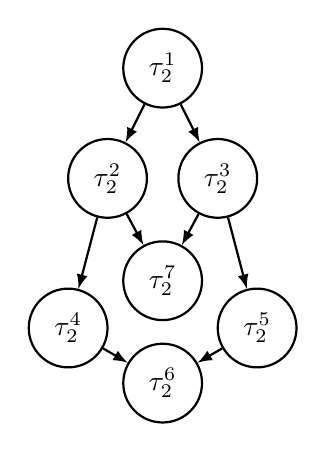
\begin{tikzpicture}
            % SEQ 1
            \node[circle, draw, thick, inner sep=0pt, minimum width=1cm] (t5) at (0,0) {$\tau_2^1$};
            \node[circle, draw, thick, inner sep=0pt, minimum width=1cm] (t6) at (-0.7,-1.4) {$\tau_2^2$};
            \node[circle, draw, thick, inner sep=0pt, minimum width=1cm] (t7) at (0.7,-1.4) {$\tau_2^3$};
            % SEQ 2
                \node[circle, draw, thick, inner sep=0pt, minimum width=1cm] (t8) at (-1.2,-3.3) {$\tau_2^4$};
            \node[circle, draw, thick, inner sep=0pt, minimum width=1cm] (t9) at (1.2,-3.3) {$\tau_2^5$};
            \node[circle, draw, thick, inner sep=0pt, minimum width=1cm] (t10) at (0,-4) {$\tau_2^6$};
            % SEQ 3
            \node[circle, draw, thick, inner sep=0pt, minimum width=1cm] (t11) at (0,-2.7) {$\tau_2^7$};
    
            % SEQ 1
            \draw[>=latex, thick,->] (t5)--(t6);
            \draw[>=latex, thick,->] (t5)--(t7);
            % SEQ 2
            \draw[>=latex, thick,->] (t8)--(t10);
            \draw[>=latex, thick,->] (t9)--(t10);
    
            % SEQ 1 -> SEQ 2
            \draw[>=latex, thick,->] (t6)--(t8);
            \draw[>=latex, thick,->] (t7)--(t9);
            % SEQ 1 -> SEQ 3
            \draw[>=latex, thick,->] (t6)--(t11);
            \draw[>=latex, thick,->] (t7)--(t11);
        \end{tikzpicture}
    };
\end{tikzpicture}

        \caption{Relations de précédence}
        \label{fig_resumeFr_appModelPrecs}
    \end{subfigure}
    \begin{subfigure}[b]{0.49\linewidth}
        \centering
        
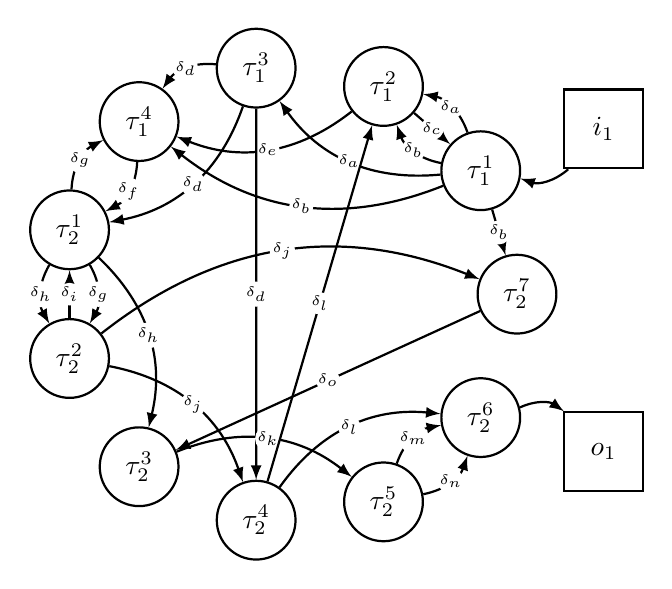
\begin{tikzpicture}
\tikzset{edgelabel/.style={fill=white, circle, inner sep=0pt, minimum size=0pt}}
\foreach \n in {1,2,...,4}{
    \node[ circle, draw, thick, inner sep=0pt, minimum width=1cm] (t\n)  at (\n*360/11: 2.9cm) {$\tau_1^{\n}$};
}
\foreach \n in {5,6,...,11}{
    \pgfmathsetmacro\result{\n - 4}
    \node[circle, draw, thick, inner sep=0pt, minimum width=1cm] (t\n)  at (\n*360/11: 2.9cm) {$\tau_2^{\pgfmathprintnumber{\result}}$};
}
\node[draw, thick, rectangle, inner sep=0pt, minimum size=1cm] (i1) at(4,2.1) {$i_1$};
\node[draw, thick, rectangle, inner sep=0pt, minimum size=1cm] (o1) at(4,-2.) {$o_1$};
\draw[-latex, thick, bend left] (i1) edge node[midway] {} (t1) ;
\draw[-latex, thick, bend left] (t10) edge node[midway] {} (o1) ;

\draw[-latex, thick, bend right] (t1) edge node[midway, edgelabel] {\tiny $\delta_a$} (t2) ;
\draw[-latex, thick, bend left] (t1) edge node[midway, edgelabel] {\tiny $\delta_b$} (t2);
\draw[-latex, thick, bend left] (t1) edge node[midway, edgelabel] {\tiny $\delta_a$} (t3);
\draw[-latex, thick, bend left] (t1) edge node[midway, edgelabel] {\tiny $\delta_b$} (t4);
\draw[-latex, thick] (t1) -- node[midway, edgelabel] {\tiny $\delta_b$} (t11);

\draw[-latex, thick] (t2) -- node[midway, edgelabel] {\tiny $\delta_c$} (t1);
\draw[-latex, thick, bend left] (t2) edge node[midway, edgelabel] {\tiny $\delta_e$} (t4);

\draw[-latex, thick, bend left] (t3) edge node[midway, edgelabel] {\tiny $\delta_d$} (t5);
\draw[-latex, thick, bend right] (t3) edge node[midway, edgelabel] {\tiny $\delta_d$} (t4);
\draw[-latex, thick] (t3) -- node[midway, edgelabel] {\tiny $\delta_d$} (t8);

\draw[-latex, thick, bend left] (t4) edge node[midway, edgelabel] {\tiny $\delta_f$} (t5);

\draw[-latex, thick, bend left] (t5) edge node[midway, edgelabel] {\tiny $\delta_g$} (t4);
\draw[-latex, thick, bend left] (t5) edge node[midway, edgelabel] {\tiny $\delta_g$} (t6);
\draw[-latex, thick, bend right] (t5) edge node[midway, edgelabel] {\tiny $\delta_h$} (t6);
\draw[-latex, thick, bend left] (t5) edge node[midway, edgelabel] {\tiny $\delta_h$} (t7);

\draw[-latex, thick] (t6) -- node[midway, edgelabel] {\tiny $\delta_i$} (t5);
\draw[-latex, thick, bend left] (t6) edge node[midway, edgelabel] {\tiny $\delta_j$} (t8);
\draw[-latex, thick, bend left] (t6) edge node[midway, edgelabel] {\tiny $\delta_j$} (t11);

\draw[-latex, thick, bend left] (t7) edge node[midway, edgelabel] {\tiny $\delta_k$} (t9);

\draw[-latex, thick] (t8) -- node[midway, edgelabel] {\tiny $\delta_l$} (t2);
\draw[-latex, thick, bend left] (t8) edge node[midway, edgelabel] {\tiny $\delta_l$} (t10);

\draw[-latex, thick, bend left] (t9) edge node[midway, edgelabel] {\tiny $\delta_m$} (t10);
\draw[-latex, thick, bend right] (t9) edge node[midway, edgelabel] {\tiny $\delta_n$} (t10);

\draw[-latex, thick] (t11) -- node[midway, edgelabel] {\tiny $\delta_o$} (t7);

\end{tikzpicture}

        \caption{Échanges de données et buffers I/O}
        \label{fig_resumeFr_appModelDataflow}
    \end{subfigure}
    \caption{Exemple de modèle d'application}
    \label{fig_resumeFr_appModelExample}
\end{figure}

\subsection{Modèle d'application}
\label{ssec_resumeFr_appModel}
Le modèle d'application considéré dans cette thèse est représentatif des applications de contrôle existantes à Airbus. Une application est une paire $<\tau,\delta>$ où $\tau$ est un ensemble fini de tâches et $\delta$ un ensemble fini de données. Chacune des tâches comprises dans $\tau = \{ \tau_1 , \ldots , \tau_n \}$ est définie par $\tau_i = <S_i , P_i , T_i>$ avec:
\begin{itemize}
    \item $S_i = \{ \tau_i^1 , \ldots , \tau_i^{n_i} \}$ un ensemble de $n_i$ sous-tâches. Toutes les sous-tâches sont activées simultanément à l'activation de $\tau_i$ et elles partagent toutes la même échéance implicite égale à la période de $\tau_i$. Chaque sous-tâche est modélisée par un quadruplet $\tau_i^j = < C_i^j, M_i^j, I_i^j, O_i^j >$ avec:
        \begin{itemize}
            \item $C_i^j$ le temps d'exécution pire-cas de $\tau_i^j$;
            \item $M_i^j$ l'empreinte mémoire de $\tau_i^j$, c'est-à-dire la somme de la taille de son code et de ses données statiques et rémanentes;
            \item $I_i^j$ et $O_i^j$ respectivement les buffers d'entrée et de sortie dans lesquels $\tau_i^j$ va lire et/ou écrire pour dialoguer avec les composants externes tels que la mémoire DDR-SDRAM.
        \end{itemize}
    \item $P_i \in S_i \times S_i$ un ensemble de paires ordonnées de sous-tâches représentant des relations de précédence contraignant l'ordre dans lequel elles peuvent être exécutées. Plus précisément, $(\tau_i^x,\tau_i^y) \in P_i$ signifie que $\tau_i^x$ doit terminer son exécution avant que $\tau_i^y$ puisse démarrer. $P_i$ impose une relation d'ordre partiel (par conséquent acyclique) entre les sous-tâches qui peut être représentée par un Graphe Orienté Acyclique (ou \emph{DAG} en anglais).
    \item $T_i$ la période de $\tau_i$. $T_i$ sert également de contrainte d'échéance implicite pour l'ensemble des sous-tâches de $\tau_i$.
\end{itemize}

Nous définissons \emph{l'hyper-période} de ce système de tâches comme $H = \underset{i \in [1,n]}{ppcm} (T_i)$ où $ppcm$ est la fonction renvoyant le plus petit commun multiple.

Les données $\delta = \{ \delta_1 , \ldots , \delta_m \}$ sont produites et consommées par les sous-tâches composant l'application. En définissant $S = \underset{\tau_i \in \tau}{\bigcup} S_i$ comme l'ensemble de toutes les sous-tâches, chaque donnée $\delta_k$ peut être définie par un triplet $\delta_k = <m_k , prod, cons>$ où:
\begin{itemize}
    \item $m_k$ représente la taille de la donnée;
    \item $prod : \delta \mapsto S$ associe chaque donnée avec la sous-tâche qui la produit;
    \item $cons : \delta \mapsto 2^S$ associe chaque donnée avec un ensemble de sous-tâches la consommant.
\end{itemize}

Toute paire de sous-tâches, même si non-contraintes par une relation de précédence, peut échanger des données. En revanche, dans notre modèle, toute paire de sous-tâches soumise à une relation de précédence implique systématiquement que les sous-tâches échangent au moins une donnée.

Notre modèle ne permet pas d'imposer de contrainte de précédence entre des sous-tâches n'appartenant pas à la même tâche. Ainsi, l'ordre de production et de consommation des données partagées par plusieurs tâches ne peut pas être contraint. Ici, l'hypothèse sous-jacente est que l'utilisation qui est faite de ces données inter-tâches est fonctionnellement robuste au plus grand délai possible entre leur production et leur consommation. Notre modèle impose que la consommation d'une donnée soit toujours celle de la valeur la plus fraîche. Ainsi, le délai production-consommation maximum d'une donnée est égal à la période de la sous-tâche productrice.

\begin{exemple}[Modèle d'application]
    \label{ex_resumeFr_appModel}

    Nous considérons une application composée de 2 tâches $\tau_1$ et $\tau_2$ qui sont respectivement composées de 4 et 7 sous-tâches avec des périodes  $T_1 = 24$ et $T_2=48$. Les 11 sous-tâches échangent 15 données et lisent et écrivent dans 1 buffer d'entrée $i_1$ et 1 buffer de sortie $o_1$.
    Les relations de précédence ainsi que les échanges de données sont représentés sur la Figure~\ref{fig_resumeFr_appModelExample}. Les paramètres des sous-tâches sont listés dans le tableau~\ref{table_resumeFr_tableTasksetExample} (ou \emph{ck} représente un nombre de cycle d'horloge).

    \begin{table}[]
        \centering
        \begin{tabular*}{0.8\linewidth}{@{\extracolsep{\fill}}  c c c c c }
            \hline
            Sous-tâches & $C_i^j$ (en ck) & $M_i^j$ (en KiB) & $I_i^j$ & $O_i^j$ \\
            \hline
            $\tau_1^1$ & 500    & 519  & $i_1$          & $\varnothing$  \\
            $\tau_1^2$ & 500    & 397  & $\varnothing$  & $\varnothing$  \\ 
            $\tau_1^3$ & 700    & 642  & $\varnothing$  & $\varnothing$  \\ 
            $\tau_1^4$ & 400    & 262  & $\varnothing$  & $\varnothing$  \\ 
            $\tau_2^1$ & 1,000  & 287  & $\varnothing$  & $\varnothing$  \\ 
            $\tau_2^2$ & 400    & 799  & $\varnothing$  & $\varnothing$  \\ 
            $\tau_2^3$ & 500    & 542  & $\varnothing$  & $\varnothing$  \\ 
            $\tau_2^4$ & 800    & 764  & $\varnothing$  & $\varnothing$  \\ 
            $\tau_2^5$ & 900    & 490  & $\varnothing$  & $\varnothing$  \\ 
            $\tau_2^6$ & 500    & 399  & $\varnothing$  & $o_1$  \\ 
            $\tau_2^7$ & 600    & 12   & $\varnothing$  & $\varnothing$  \\ 
            \hline
        \end{tabular*}
        \caption{Paramètres des sous-tâches}
        \label{table_resumeFr_tableTasksetExample}
    \end{table}
\end{exemple}







\subsection{Architecture du \mppalong}

Le \mppalong~\cite{kalray_mppa} est un processeur pluri-c\oe{}urs comprenant 288 c\oe{}urs sur une seule puce. Il est particulièrement adapté aux applications temps réel nécessitant une puissance de calcul importante de part sa faible dissipation thermique ainsi que ses bonnes propriétés temporelles. Dans le cadre de cette thèse, nous utilisons la deuxième version du \mppalong dénommée \emph{Bostan}.

Comme montré sur la Figure~\ref{fig_resumeFr_MPPANoCtopology}, le \mppalong comporte 16 \emph{clusters} dédiés au calcul (les $C_i$ sur la figure). De plus, à la périphérie du processeur se trouvent 4 clusters \emph{IO}, c'est-à-dire dédiés à la gestion des interactions avec les composants externes tels que la DDR-SDRAM ou le réseau Ethernet. Les clusters sont interconnectés par 2 Réseaux-sur-Puces (ou \emph{NoC} en anglais) qui permettent des communications point à point par l'envoi de message.


%\subsubsection{Vue d'ensemble}
\begin{figure}
    \centering
    \scalebox{1.5}{\begin{picture}(210,210)
    \put(0,0){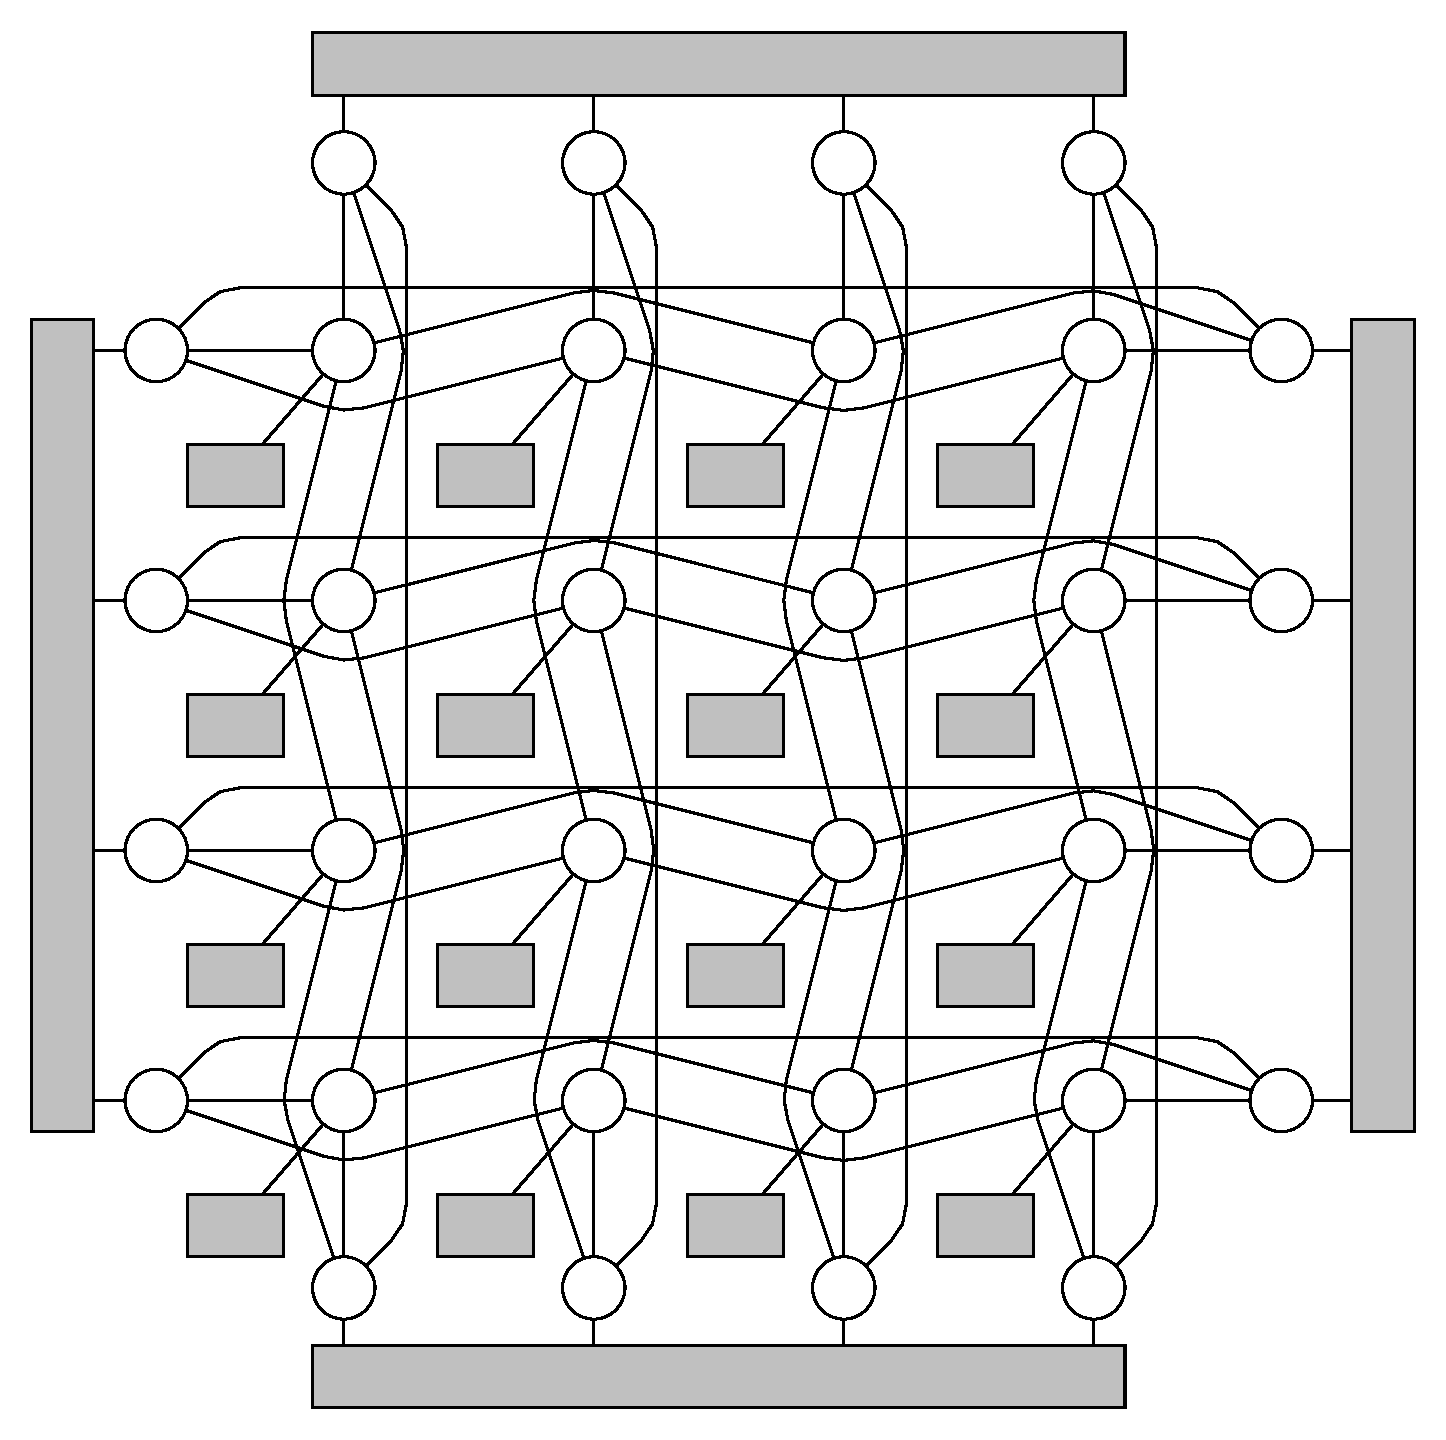
\includegraphics[width=210px]{imgs/pdf/all_MPPA_NoC_overview.pdf}}
    % I/O Tiles
    \put(80,7){\scriptsize \textit{Cluster IO sud}}
    \put(78,198){\scriptsize \textit{Cluster IO nord}}
    \put(6,77){\scriptsize \rotatebox{90}{\textit{Cluster IO ouest}}}
    \put(199,128){\scriptsize \rotatebox{270}{\textit{Cluster IO est}}}
    % Clusters 0-3
    \put(30, 139){\scriptsize $C_0$}
    \put(66, 139){\scriptsize $C_1$}
    \put(103,139){\scriptsize $C_2$}
    \put(139,139){\scriptsize $C_3$}
    % Clusters 4-7
    \put(30, 102){\scriptsize $C_4$}
    \put(66, 102){\scriptsize $C_5$}
    \put(103,102){\scriptsize $C_6$}
    \put(139,102){\scriptsize $C_7$}
    % Clusters 8-11
    \put(30, 66){\scriptsize $C_8$}
    \put(66, 66){\scriptsize $C_9$}
    \put(101,66){\scriptsize $C_{10}$}
    \put(137,66){\scriptsize $C_{11}$}
    % Clusters 12-15
    \put(28, 29){\scriptsize $C_{12}$}
    \put(64, 29){\scriptsize $C_{13}$}
    \put(101,29){\scriptsize $C_{14}$}
    \put(137,29){\scriptsize $C_{15}$}

    % Routers 0-3
    \put(47, 158){\scalebox{0.7}{\tiny $R_0$}}
    \put(83, 158){\scalebox{0.7}{\tiny $R_1$}}
    \put(120,158){\scalebox{0.7}{\tiny $R_2$}}
    \put(156,158){\scalebox{0.7}{\tiny $R_3$}}
    % Routers 4-7
    \put(47, 122){\scalebox{0.7}{\tiny $R_4$}}
    \put(83, 122){\scalebox{0.7}{\tiny $R_5$}}
    \put(120,122){\scalebox{0.7}{\tiny $R_6$}}
    \put(156,122){\scalebox{0.7}{\tiny $R_7$}}
    % Routers 8-11
    \put(47, 85){\scalebox{0.7}{\tiny $R_8$}}
    \put(83, 85){\scalebox{0.7}{\tiny $R_9$}}
    \put(119,85){\scalebox{0.7}{\tiny $R_{10}$}}
    \put(155,85){\scalebox{0.7}{\tiny $R_{11}$}}
    % Routers 12-15
    \put(46, 49){\scalebox{0.7}{\tiny $R_{12}$}}
    \put(82, 49){\scalebox{0.7}{\tiny $R_{13}$}}
    \put(119,49){\scalebox{0.7}{\tiny $R_{14}$}}
    \put(155,49){\scalebox{0.7}{\tiny $R_{15}$}}
    % Routers North
    \put(47, 185){\scalebox{0.7}{\tiny $R^n_0$}}
    \put(83, 185){\scalebox{0.7}{\tiny $R^n_1$}}
    \put(119,185){\scalebox{0.7}{\tiny $R^n_2$}}
    \put(156,185){\scalebox{0.7}{\tiny $R^n_3$}}
    % Routers South
    \put(47, 21){\scalebox{0.7}{\tiny $R^s_0$}}
    \put(83, 21){\scalebox{0.7}{\tiny $R^s_1$}}
    \put(119,21){\scalebox{0.7}{\tiny $R^s_2$}}
    \put(156,21){\scalebox{0.7}{\tiny $R^s_3$}}
    % Routers West
    \put(19,158){\scalebox{0.7}{\tiny $R^o_0$}}
    \put(19,122){\scalebox{0.7}{\tiny $R^o_1$}}
    \put(19, 85){\scalebox{0.7}{\tiny $R^o_2$}}
    \put(19, 49){\scalebox{0.7}{\tiny $R^o_3$}}
    % Routers East
    \put(183,158){\scalebox{0.7}{\tiny $R^e_0$}}
    \put(183,122){\scalebox{0.7}{\tiny $R^e_1$}}
    \put(183, 85){\scalebox{0.7}{\tiny $R^e_2$}}
    \put(183, 49){\scalebox{0.7}{\tiny $R^e_3$}}

    \end{picture}
}
    \caption{Architecture du \mppalong}
    \label{fig_resumeFr_MPPANoCtopology}
\end{figure} 

\subsubsection{Les clusters de calcul}

Comme cela est montré sur la Figure~\ref{fig_resumeFr_MPPAComputeCluster}, chaque cluster de calcul comporte:
\begin{itemize}
    \item 16 c\oe{}urs de calcul, appelés les \emph{Processing Elements} (ou \emph{PE}). Les PEs sont dédiés à l'exécution de code utilisateur.
    \item un c\oe{}ur supplémentaire, appelé le \emph{Resource Manager} (ou \emph{RM}) qui gère l'ensemble des ressources locales du cluster.
    \item une unité de débogage, la \emph{Debug and Support Unit} (ou \emph{DSU}) qui facilite le développement et permet notamment d'utiliser le JTAG.
    \item un contrôleur \emph{DMA} (pour \emph{Direct Memory Access}) qui permet l'envoi de données au travers du NoC.
    \item 2MiB de SRAM partagée qui est organisée en 16 bancs indépendants.
    \item 1 interface d'accès à chacun des deux NoCs.
\end{itemize}
\begin{figure}
    \centering
    \scalebox{0.8}{
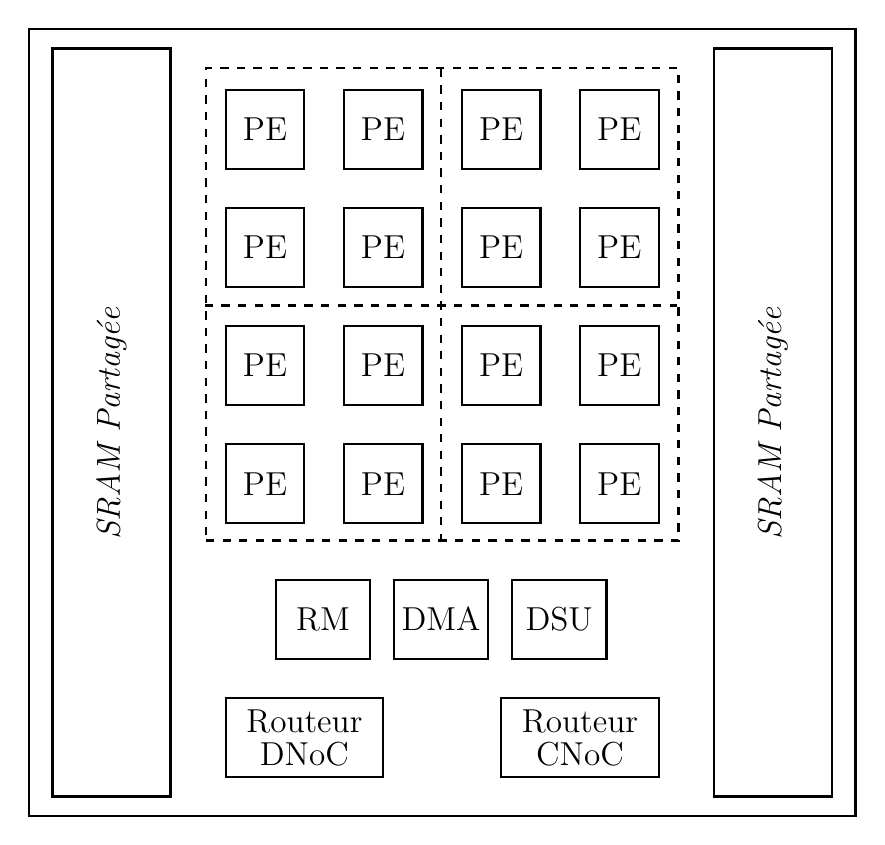
\begin{tikzpicture}[font={\fontsize{13pt}{12}\selectfont}]

    \node[rectangle, draw, color=black, thick, anchor=south west, minimum width=10.5cm, minimum height=10cm, inner sep=0pt] at (0,0.25) {};

    \node[rectangle, draw, color=black, thick, anchor=north west, minimum width=9.5cm, minimum height=1.5cm, inner sep=0pt, rotate=90] at (0.3,0.5) {\textit{SRAM Partagée}};
    \node[rectangle, draw, color=black, thick, anchor=north west, minimum width=9.5cm, minimum height=1.5cm, inner sep=0pt, rotate=90] at (8.7,0.5) {\textit{SRAM Partagée}};
    
%    \draw[color=black, thick, dashed] (0.25, 1.50) -- (1.75, 1.50); 
%    \draw[color=black, thick, dashed] (0.25, 2.75) -- (1.75, 2.75); 
%    \draw[color=black, thick, dashed] (0.25, 4) -- (1.75, 4); 
%    \draw[color=black, thick, dashed] (0.25, 5.25) -- (1.75, 5.25); 
%    \draw[color=black, thick, dashed] (0.25, 6.5) -- (1.75, 6.50); 
%    \draw[color=black, thick, dashed] (0.25, 7.75) -- (1.75, 7.75); 
%    \draw[color=black, thick, dashed] (0.25, 9) -- (1.75, 9); 


    \node[rectangle, draw, color=black, thick, anchor=north west, minimum width=1cm, minimum height=1cm, inner sep=0pt] at (2.5,9.5) {PE};
    \node[rectangle, draw, color=black, thick, anchor=north west, minimum width=1cm, minimum height=1cm, inner sep=0pt] at (4,  9.5) {PE};
    \node[rectangle, draw, color=black, thick, anchor=north west, minimum width=1cm, minimum height=1cm, inner sep=0pt] at (5.5,9.5) {PE};
    \node[rectangle, draw, color=black, thick, anchor=north west, minimum width=1cm, minimum height=1cm, inner sep=0pt] at (7,  9.5) {PE};

    \node[rectangle, draw, color=black, thick, anchor=north west, minimum width=1cm, minimum height=1cm, inner sep=0pt] at (2.5,8) {PE};
    \node[rectangle, draw, color=black, thick, anchor=north west, minimum width=1cm, minimum height=1cm, inner sep=0pt] at (4,  8) {PE};
    \node[rectangle, draw, color=black, thick, anchor=north west, minimum width=1cm, minimum height=1cm, inner sep=0pt] at (5.5,8) {PE};
    \node[rectangle, draw, color=black, thick, anchor=north west, minimum width=1cm, minimum height=1cm, inner sep=0pt] at (7,  8) {PE};
    
    \node[rectangle, draw, color=black, thick, anchor=north west, minimum width=1cm, minimum height=1cm, inner sep=0pt] at (2.5,6.5) {PE};
    \node[rectangle, draw, color=black, thick, anchor=north west, minimum width=1cm, minimum height=1cm, inner sep=0pt] at (4,  6.5) {PE};
    \node[rectangle, draw, color=black, thick, anchor=north west, minimum width=1cm, minimum height=1cm, inner sep=0pt] at (5.5,6.5) {PE};
    \node[rectangle, draw, color=black, thick, anchor=north west, minimum width=1cm, minimum height=1cm, inner sep=0pt] at (7,  6.5) {PE};

    \node[rectangle, draw, color=black, thick, anchor=north west, minimum width=1cm, minimum height=1cm, inner sep=0pt] at (2.5,5) {PE};
    \node[rectangle, draw, color=black, thick, anchor=north west, minimum width=1cm, minimum height=1cm, inner sep=0pt] at (4,  5) {PE};
    \node[rectangle, draw, color=black, thick, anchor=north west, minimum width=1cm, minimum height=1cm, inner sep=0pt] at (5.5,5) {PE};
    \node[rectangle, draw, color=black, thick, anchor=north west, minimum width=1cm, minimum height=1cm, inner sep=0pt] at (7,  5) {PE};
    
    \node[rectangle, draw, color=black, thick, anchor=south west, minimum width=6cm, minimum height=6cm, inner sep=0pt, dashed] at (2.25,3.75) {};
    \draw[color=black, thick, dashed] (2.25, 6.75) -- (8.25, 6.75); 
    \draw[color=black, thick, dashed] (5.25, 9.755) -- (5.25, 3.75); 
    
    \node[rectangle, draw, color=black, thick, anchor=south west, minimum width=2cm, minimum height=1cm, text width=1.5cm,  align=center,inner sep=0pt] at (2.5,  0.75) {Routeur\\ DNoC};
    \node[rectangle, draw, color=black, thick, anchor=south west, minimum width=2cm, minimum height=1cm, text width=1.5cm,  align=center,inner sep=0pt] at (6,  0.75) {Routeur\\ CNoC};

    \node[rectangle, draw, color=black, thick, anchor=south, minimum width=1.2cm, minimum height=1cm, inner sep=0pt] at (3.75,  2.25) {RM};
    \node[rectangle, draw, color=black, thick, anchor=south, minimum width=1.2cm, minimum height=1cm, inner sep=0pt] at (5.25,  2.25) {DMA};
    \node[rectangle, draw, color=black, thick, anchor=south, minimum width=1.2cm, minimum height=1cm, inner sep=0pt] at (6.75,  2.25) {DSU};
    
\end{tikzpicture}
}
    \caption{Architecture d'un cluster de calcul du \mppalong}
    \label{fig_resumeFr_MPPAComputeCluster}
\end{figure}

Tous les c\oe{}urs du \mppalong sont conçus selon la même architecture (\emph{k1b} sur Bostan) laquelle repose sur un pipeline à 7 étages exécutant des bundles de 5 instructions en \emph{VLIW} (pour \emph{Very Long Instruction Word}). La fréquence d'horloge des c\oe{}urs peut être élevée jusqu'à 600MHz. Chaque c\oe{}ur peut effectuer des opérations arithmétiques sur des entiers en 32 et 64 bits ainsi que des opérations de multiplication-sommation sur des flottants en double précision. Par ailleurs, deux modes d'exécution (\emph{utilisateur} ou \emph{privilégié}) sont disponibles pour supporter l'exécution d'un système d'exploitation. Chaque c\oe{}ur dispose également d'une unité de gestion de mémoire (ou \emph{MMU} en anglais) permettant une protection et une virtualisation de la mémoire paginée. Dans les clusters de calculs, tous les c\oe{}urs disposent de caches de données et d'instructions privés (8KiB chacun) pour rendre les accès à la mémoire SRAM locale plus efficaces.

\begin{figure}
    \centering
    \scalebox{0.8}{
% 1 : x; 2: y; 3: no; 4: tikz object name
\newcommand\smemarbpe[4]{
    \node[rectangle, draw, color=black, thick, anchor=south west, minimum width=1.2cm, minimum height=1cm, inner sep=0pt] (#4) at (#1, #2) {PE#3};
    \node[rectangle, draw, color=black, thick, anchor=south west, minimum width=0.8cm, minimum height=0.5cm, inner sep=0pt] (IC#4) at (#1 + 1.2, #2) {{\small I\$}};
    \node[rectangle, draw, color=black, thick, anchor=south west, minimum width=0.8cm, minimum height=0.5cm, inner sep=0pt] (DC#4) at (#1 + 1.2, #2 + 0.5) {{\small D\$}};
}

% 1 : x; 2: y; 3: tikz object name
\newcommand\smemRRarb[3]{
    \node[circle, draw, color=black, thick, minimum size=0.7cm, inner sep=0pt] (#3) at (#1, #2) {\textit{\scriptsize RR}};
    \draw[ultra thick, ->, >=latex] (#3.west) -- ([yshift=-0.6em]#3.west); 
}

\begin{tikzpicture}[font={\fontsize{12pt}{12}\selectfont}]


    \node[rectangle, draw, color=black, thick, anchor=south west, minimum width=2cm, minimum height=1cm, inner sep=0pt] (DMARx) at (0, 0) {DMA Rx};

    \node[rectangle, draw, color=black, thick, anchor=south west, minimum width=2cm, minimum height=1cm, inner sep=0pt] (DMATx) at (0, 1.5) {DMA Tx};
    \node[rectangle, draw, color=black, thick, anchor=south west, minimum width=2cm, minimum height=1cm, inner sep=0pt] (DSU) at (0, 3) {DSU};
    \node[rectangle, draw, color=black, thick, anchor=south west, minimum width=2cm, minimum height=1cm, inner sep=0pt] (RM) at (0, 4.5) {RM};
    \smemRRarb {4.5}{3.5}{rrRM}
    \draw[thick, ->, >=latex] (RM.east) -| (rrRM.north);
    \draw[thick, ->, >=latex] (DMATx.east) -| (rrRM.south);
    \draw[thick, ->, >=latex] (DSU.east) -- (rrRM.west);

    
    \smemarbpe{0}{6}{16}{pe16}
    \smemRRarb {3}{6.5}{rrpe16}
    \draw[thick, ->, >=latex] (ICpe16.east) -- (rrpe16.220);
    \draw[thick, ->, >=latex] (DCpe16.east) -- (rrpe16.135);
    \node at (1, 7.5) {{\Huge ...}};
    
    \smemarbpe{0}{8}{2}{pe2}
    \smemRRarb {3}{8.5}{rrpe2}
    \draw[thick, ->, >=latex] (ICpe2.east) -- (rrpe2.220);
    \draw[thick, ->, >=latex] (DCpe2.east) -- (rrpe2.135);
    
    \smemarbpe{0}{9.5}{1}{pe1}
    \smemRRarb {3}{10}{rrpe1}
    \draw[thick, ->, >=latex] (ICpe1.east) -- (rrpe1.220);
    \draw[thick, ->, >=latex] (DCpe1.east) -- (rrpe1.135);


    \smemRRarb {4.5}{8.5}{rrPEs}
    \draw[thick, ->, >=latex] (rrpe1.east) -| (rrPEs.north);
    \draw[thick, ->, >=latex] (rrpe2.east) -- (rrPEs.west);
    \draw[thick, ->, >=latex] (rrpe16.east) -| (rrPEs.south);
    
    \smemRRarb {6}{6}{rrFinal}
    \draw[thick, ->, >=latex] (rrPEs.east) -| (rrFinal.north);
    \draw[thick, ->, >=latex] (rrRM.east) -| (rrFinal.south);

    \node[circle, draw, color=black, fill=black, thick, minimum size=0.15cm, inner sep=0pt] (lpint) at (7, 6) {};
    \node[circle, draw, color=black, fill=black, thick, minimum size=0.15cm, inner sep=0pt] (hpint) at (7, 5.5) {};
    \node[circle, draw, color=black, fill=black, thick, minimum size=0.15cm, inner sep=0pt] (outint) at (7.7, 6) {};
    \node at (7.4, 6.4) {{\small Priorité}};
    \draw[thick, ->, >=latex] (rrFinal.east) -- (lpint.west);
    \draw[thick, ->, >=latex] (DMARx.east) -| (hpint.south);
    \draw[thick] (hpint) -- (outint);
    
    \node[rectangle, draw, color=black, thick, anchor=south west, minimum width=2.5cm, minimum height=1cm, inner sep=0pt] (banki) at (9, 5.5) {\textit{Banc i}};
    \node[rectangle, draw, color=black, thick, anchor=south west, minimum width=2.5cm, minimum height=1cm, inner sep=0pt] at (9, 4) {\textit{Banc i+1}};
    \node[rectangle, draw, color=black, thick, anchor=south west, minimum width=2.5cm, minimum height=1cm, inner sep=0pt] at (9, 2.5) {\textit{Banc i+2}};
    \node[rectangle, draw, color=black, thick, anchor=south west, minimum width=2.5cm, minimum height=1cm, inner sep=0pt] at (9, 1) {\textit{Banc i+3}};
    \node[rectangle, draw, color=black, thick, anchor=south west, minimum width=2.5cm, minimum height=1cm, inner sep=0pt] at (9, 7) {\textit{Banc i-1}};
    \node[rectangle, draw, color=black, thick, anchor=south west, minimum width=2.5cm, minimum height=1cm, inner sep=0pt] at (9, 8.5) {\textit{Banc i-2}};
    \node[rectangle, draw, color=black, thick, anchor=south west, minimum width=2.5cm, minimum height=1cm, inner sep=0pt] at (9, 10) {\textit{Banc i-3}};

    \draw[thick, ->, >=latex] (outint.east) -- (banki.west);
    
\end{tikzpicture}
}
    \caption{Politique d'arbitrage vers la SRAM locale sur le \mppalong}
    \label{fig_resumeFr_MPPASMEMarbiter}
\end{figure}

La mémoire SRAM locale d'un cluster de calcul n'est accessible que par les éléments internes du cluster. La mémoire est découpée en 16 bancs de 128KiB chacun. Dans le cas où deux bancs sont adressés simultanément par deux masters, les chemins d'accès à chaque banc étant indépendants, aucune interférence ne se fera ressentir. En revanche, des accès concurrents au même banc subiront un arbitrage en Round-Robin hiérarchique comme montré sur la Figure~\ref{fig_resumeFr_MPPASMEMarbiter}. En règle générale, la SRAM locale peut être utilisée pour permettre des communications internes au cluster par mémoire partagée. Cependant, il est important de noter qu'aucune forme de cohérence de cache n'est assurée par le matériel et qu'il revient donc au logiciel de gérer ce problème. Pour ce faire, il est possible soit d'utiliser des instructions spécifiques permettant explicitement de purger tout ou partie du cache d'un c\oe{}ur, soit d'utiliser les MMUs des c\oe{}urs pour forcer des politiques de cachage spécifiques (\emph{Write-Through} ou \emph{Bypass} notamment) sur certaines pages mémoire. Cependant, il existe également un second moyen de communication entre les c\oe{}urs d'un même cluster. En effet, comme indiqué sur la Figure~\ref{fig_resumeFr_MPPAComputeCluster}, les PEs sont groupés par paquets de quatre au sein de chaque cluster de calcul. À l'intérieur de chaque groupe, les PEs peuvent émettre et recevoir des événements vers et depuis leurs voisins. Cela permet notamment l'implémentation de barrières de synchronisation efficaces en évitant le polling sur la mémoire SRAM locale. Par ailleurs, les PEs au sein d'un groupe disposent de facilités d'écriture dans certains registres des PEs voisins, permettant ainsi des échanges de données sans utiliser de zone de mémoire partagée.

\subsubsection{Entre les clusters}
Les communications entre les clusters se font par le passage explicite de messages ou par tirs DMA distants au travers d'un NoC. Les contrôleurs DMA se trouvant dans chaque cluster permettent de décharger les c\oe{}urs du travail d'émission et de réception des paquets NoCs. Chaque DMA dispose ainsi de 8 canaux d'émission qui peuvent être configurés indépendamment. En particulier, le choix de la route à suivre pour les paquets ainsi que les paramètres de régulation à l'injection sont spécifiques à chaque canal d'émission. Par défaut, seul le RM a la capacité d'écrire dans les registres de configuration du DMA. Les PEs peuvent être autorisés à faire de même par configuration. Le contrôleur DMA comporte un micro-moteur capable d'exécuter simultanément jusqu'à 8 threads. Chaque thread exécute des instructions issues d'un binaire résultant de la compilation d'un micro-code écrit dans un langage d'assemblage léger et spécifique à Kalray. En réception, chaque DMA dispose de 256 canaux qui peuvent, eux aussi, être configurés indépendamment. Ainsi, chaque canal de réception peut être associé à une zone de mémoire locale de taille finie dans laquelle seront écrits les messages entrant sur ce canal. Par ailleurs, les canaux de réception peuvent être configurés pour envoyer un événement au RM dans certaines situations telles que la réception d'un paquet notifiant la fin d'une transmission ou lorsque la quantité de données reçues dépasse un certain seuil.

Les deux NoCs disponibles sur le \mppalong comportent la même topologie en tore 2D comme représenté sur la Figure~\ref{fig_resumeFr_MPPANoCtopology}. Le \emph{DNoC} (ou \emph{Data-NoC}) est dédié à l'envoi des données volumineuses par l'intermédiaire du DMA. Le \emph{CNoC} (ou \emph{Control-NoC}) est quant à lui dédié à l'envoi de messages de contrôle courts qui peuvent notamment être utilisés pour effectuer des synchronisations inter-clusters. Les 2 NoCs suivent une politique de routage en wormhole avec un choix des routes à la source.


\subsubsection{Adéquation aux contraintes avioniques}
Le choix du \mppalong comme cible privilégiée pour l'application de ce travail de thèse est motivé par plusieurs raisons aussi bien techniques que non-techniques. Tout d'abord, la faible dissipation thermique du \mppalong est un premier atout majeur. Une faible consommation énergétique permet non seulement de réduire la consommation de carburant de l'avion mais surtout de faciliter la conception des cartes électroniques embarquées et de simplifier leur certification. En effet, il semble que, sous certaines conditions d'utilisation, le \mppalong dissipe une puissance suffisamment faible pour permettre de le refroidir passivement et par conséquent d'éviter le coût additionnel lié à la certification d'une solution de refroidissement active.

Deuxièmement, les propriétés temporelles du \mppalong semblent être particulièrement adaptées à son utilisation dans un contexte temps réel dur. Il a notamment été démontré dans le cadre du projet {\sc Certainty}~\cite{Certainty} que les c\oe{}urs de calcul du \mppalong exhibent une propriété de \emph{full timing compositionality}. En conséquence, le calcul des temps d'exécution pire-cas des programmes est simplifié et peut être effectué par la composition de plusieurs sous-analyses évitant ainsi de devoir effectuer une seule analyse coûteuse du système complet.

Troisièmement, il apparaît que très peu d'opérations sont effectuées de manière implicite sur le \mppalong. L'absence de cohérence de cache matérielle et la capacité à envoyer des messages au travers du NoC par la programmation du DMA qui lui-même exécute un code modifiable en sont de bons exemples. De manière générale, la programmabilité de la plateforme est excellente et la capacité de contrôle par le logiciel est importante. Même si cette spécificité ne simplifie clairement pas la programmation haut niveau, cela apparaît comme un véritable atout dans un contexte avionique où la capacité à maîtriser de la plateforme est un enjeu particulièrement critique.

Enfin, \kalray en tant qu'entreprise s'est montré particulièrement enclin à communiquer à ses clients des informations précises et détaillées sur leur plateforme. Dans le cas où le calcul des temps d'exécution pire-cas serait effectué par analyse statique, des modélisations fines du matériel seront nécessaires. Par conséquent, être capable d'obtenir les informations adéquates pour la construction de ces modèles s'avère être particulièrement important d'un point de vue industriel.

%\section{État de l'art}
%\subsection{Borner les temps d'exécution}
%\subsubsection{Le calcul du temps d'exécution pire-cas}
%\subsubsection{Les ressources partagées sur pluri-c\oe{}urs}
%\subsubsection{Prise en compte de la prédictibilité lors de la conception}

%\subsection{Ordonnancement hors-ligne de tâches parallèles}
%\subsubsection{Ordonnancement hors-ligne de tâches DAG}
%\subsubsection{Placement hors-ligne sur des architectures distribuées}

\subsection{Synthèse}
Les entrées de notre travail sont de deux natures. Nous avons d'une part un modèle d'application sous la forme d'un ensemble de tâches parallélisables et d'autre part une plateforme d'exécution puissante bien que complexe avec le \mppalong. Notre objectif sera ici de définir le moyen d'exploiter la puissance de calcul parallèle du \mppalong pour permettre non seulement l'exécution prédictible de plusieurs applications temporellement isolées les unes des autres mais également pour supporter l'augmentation des besoins en puissance de calcul des systèmes avioniques par la distribution d'applications sur plusieurs clusters du processeur. En outre, nous prendrons en compte les contraintes inhérentes au contexte industriel telles que la nécessité d'avoir des outils fonctionnant en temps raisonnable ou le besoin de solution reposant majoritairement sur le pré-calcul pour limiter le coût de certification d'un code volumineux qui prendrait les décisions en-ligne.

\section{État de l'art}

Deux problématiques majeures se posent pour ce travail. Tout d'abord, considérant un composant sur étagère non-conçu spécifiquement pour le temps réel, il sera nécessaire d'adopter une stratégie logicielle assurant la maîtrise de plateforme matérielle afin de garantir des exécutions prédictibles. Et deuxièmement, au vue de la complexité des applications industrielles visées, il semble nécessaire de permettre le placement et l'ordonnancement d'applications parallèles de façon automatisée et efficace. Nous détaillons les travaux existant sur ces deux sujets dans cette section.

\subsection{Maîtrise du matériel}
La problématique de la maîtrise de processeurs sur étagère à des fins d'exécution temps réel n'est pas nouvelle. Essentiellement deux types de stratégies logicielles ont été proposées dans ce cadre. D'abord, il y a les approches uniquement basées sur l'utilisation d'un logiciel de contrôle. Dans ce cas, les applications sont exécutées sans les modifier aucunement et seule une couche basse de logiciel garantit un accès ordonné à des ressources sensibles. Dans cette idée, Fisher~\cite{FisherWP} a proposé le premier logiciel de contrôle permettant la certification d'applications au niveau SIL 4 des régulations ferroviaires sur un processeur multi-c\oe{}urs. Dans son approche, les tâches doivent être classifiées comme critiques ou non-critiques. Ensuite, le temps est découpé en slots successifs. Certains slots sont marqués comme critiques et les autres comme non-critiques. L'idée est que, lors des slots non-critiques, tous les c\oe{}urs peuvent être utilisés simultanément pour l'exécution de tâches non-critiques pour lesquelles les contentions d'accès aux ressources partagées ne sont pas problématiques. Lors de slots critiques en revanche, seul un c\oe{}ur est habilité à exécuter une tâche critique pendant que les autres c\oe{}urs sont maintenus inactifs. Ce faisant, la tâche critique s'exécutant seule ne subira aucunte interférence d'accès aux différentes ressources du processeur. Cela permet d'obtenir des garanties temporelles fermes sur l'exécution des tâches critiques mais peut aussi amener à des faibles utilisations des c\oe{}urs, et en particulier lorsque beaucoup de tâches critiques sont présentes.

Dans~\cite{jean12}, Jean \etal ont proposé {\sc Marthy}, un hyperviseur permettant d'assurer un partitionnement robuste entre plusieurs applications concurrentes s'exécutant sur un processeur multi-c\oe{}urs. {\sc Marthy} est verrouillé dans les caches des c\oe{}urs et détecte l'utilisation d'instructions \emph{sensibles}, c'est-à-dire qui impactent le trafic traversant l'interconnect ou bien l'état des autres c\oe{}urs. Lorsque une telle instruction est utilisée par une application, {\sc Marthy} reprend le contrôle du c\oe{}ur et attend le début d'un créneau d'accès préalablement alloué à ce c\oe{}ur pour exécuter l'instruction. Les créneaux d'accès alloués aux c\oe{}urs n'ayant pas de recouvrement temporel, les conflits d'accès aux ressources partagées sont éliminés. Ainsi, {\sc Marthy} permet d'apporter des garanties temps réel dur à des applications tout en permettant l'exécution simultanée de plusieurs tâches critiques sur des c\oe{}urs différents (tant qu'elles n'accèdent pas aux ressources partagées). Cette approche résout (au moins partiellement) les problèmes identifiés pour l'approche précédente mais il apparaît que certaines applications souffrent d'importantes pertes de performance avec {\sc Marthy}~\cite{Jean2015}. En effet, ces applications peuvent être utilisées sans modification mais peuvent subir des latences d'accès importantes aux ressources partagées, et en particulier lorsqu'elles sont mal alignées temporellement avec le slot d'accès de leur c\oe{}ur.

Dans~\cite{Yun2013}, Yun \etal ont proposé Memguard, un système de régulation fournissant une bande passante mémoire garantie aux applications s'exécutant sur une cible multi-c\oe{}urs. Pour cela, chaque c\oe{}ur est associé à un budget qui contient un nombre maximal d'accès au bus pour une fenêtre temporelle donnée. Les accès de chaque c\oe{}ur sont comptés par des compteurs matériels évaluant le nombre de miss dans le cache de dernier niveau. Lorsque le budget est atteint, une interruption est générée et le c\oe{}ur est stoppé jusqu'à la fin de la fenêtre en cours. Ce faisant, en allouant des budgets aux c\oe{}urs dont la somme est inférieure à la bande passante de la mémoire, il est possible de fournir des garanties qui faciliteront par la suite l'évaluation des WCETs. Toutefois, Memguard intègre un mécanisme de redistribution de la bande passante non-utilisée aux applications \emph{best-effort} qui effectue des spéculations sur l'utilisation de la mémoire par les c\oe{}urs afin de réallouer la bande passante. Malheureusement, cette spéculation peut parfois être optimiste et ainsi fragiliser les garanties apportées aux applications temps réel. \\


D'une manière générale, les trois travaux mentionnés précédemment reposent uniquement sur l'utilisation d'un logiciel de contrôle et ne requièrent pas de modifications des applications. D'autres travaux sont basés sur une idée différente où la modification des applications ferait partie de la stratégie de contrôle. L'objectif est généralement d'exploiter plus efficacement le matériel afin d'obtenir des performances accrues. Pellizzoni~\etal ont présenté \emph{PREM} (pour \emph{Predictable Execution Model})~\cite{Pellizzoni2011_PREM} en suivant cette philosophie. Avec PREM, il est demandé aux développeurs d'applications d'annoter leur code pour mentionner les sections \emph{predictibles}. Ainsi, les sections prédictibles sont découpées par le compilateur en phases mémoire et en phases d'exécution. L'idée est qu'une phase mémoire correspond à une étape de chargement de code et de données en cache et que les phases d'exécution utilisent le code et les données préalablement chargées sans jamais faire de miss en cache. Les phases mémoire des tâches sont ordonnancées de façon à éviter les conflits d'accès aux ressources et les phases d'exécution sont ordonnancées sur les c\oe{}urs avec la garantie qu'elles se feront sans interruptions liées à des ressources externes. 

Les concepts introduits dans PREM on été étendus par Durrieu \etal dans~\cite{Durrieu2014}. Leur objectif est de permettre le portage d'une application industrielle de Thales sur un multi-c\oe{}urs COTS~\cite{TMS320C6678}. Les auteurs supposent un modèle de tâche \emph{Acquisition, Exécution, Restitution} (ou \emph{AER}) ou les exécutions et communications sont découplées. Les caches L2 du processeur sont configurés en SRAM afin de permettre lors des phases d'acquisition le chargement du code et des données requises pour la phase d'exécution suivante. Celle-ci se poursuit alors en isolation sur un c\oe{}ur sans accéder aux ressources partagées du processeur. Enfin, les données produites sont propagées en mémoire DDR-SDRAM externe lors des phases de restitution. Avec AER, les phases d'acquisition et de restitution sont ordonnancées sans recouvrement temporel pour améliorer la prédictibilité d'accès aux ressources partagées et les exécutions concurrentes sont acceptées. 

D'autres travaux\cite{Jegu2012,Tabish2016} sont basés sur ces concepts similaires afin de garantir des exécutions prédictibles sur des processeurs mono- ou multi-c\oe{}urs. Cependant, que ce soit avec ou sans modification d'application, la maîtrise d'un processeur \emph{pluri}-c\oe{}urs COTS avec une stratégie de contrôle purement logicielle est un domaine qui reste aujourd'hui relativement peu exploré. La résolution de ce problème est le premier objectif de notre travail.

\subsection{Placement et ordonnancement d'applications}
Le placement et l'ordonnancement d'applications sur des plateformes pluri-c\oe{}urs est un sujet de recherche en plein essor. Parmi les travaux visant spécifiquement le \mppalong, Giannopoulou \etal~\cite{Giannopoulou2015} ont proposé l'application d'une politique d'ordonnancement appelée \emph{Flexible Time-Triggered Scheduling} (\emph{FTTS}) initialement présentée dans~\cite{Giannopoulou2013_EMSOFT}. Un ordonnancement FTTS est composé d'une succession de \emph{frames} d'une durée préalablement figée. Cette séquence de frames est répétée indéfiniment sur un cycle d'ordonnancement dont la durée est appelée hyper-période. Chaque frame est découpée en sous-frames de durées variables. Les tâches sont exécutées dans les sous-frames. La stratégie proposée repose sur l'allocation des tâches de haute criticité aux sous-frames qui débutent les frames. Inversement, les tâches peu critiques sont exécutées en fin de frames. Ainsi, les tâches hautement critiques sont exécutées sans encombre et les peu critiques le sont (en mode nominal, en mode dégradé ou ne le sont pas) si le temps restant dans la frame le permet. Avec FTTS, une exécution sûre des tâches les plus critiques est garantie et une exécution opportuniste des tâches peu critique est permise. Toutefois, il est nécessaire que les WCETs des tâches restent tous dans le même ordre de grandeur pour minimiser les temps d'attente dans les sous-frames. En plus du travail d'ordonnancement, les auteurs ont effectué une analyse conjointe des interférences d'accès à la SRAM locale des clusters de calcul et des pires temps de traversée des paquets NoC en utilisant le Calcul Réseau~\cite{LeBoudec2001, Cruz91}. Malheureusement, ces travaux n'ont, à notre connaissance, pas été implémentés sur cible réelle et n'ont pas été évalués expérimentalement. En particulier, la complexité du logiciel de contrôle supportant l'exécution des frames et sous-frames n'est pas décrite.

Dans~\cite{Becker16}, Becker \etal ont proposé une méthode d'ordonnancement au sein d'un seul cluster du \mppalong. Ils supposent un modèle de tâche suivant la philosophie d'AER. Chaque tâche est composée de 3 phases. Ainsi, le WCET d'une tâche est décomposé en $C_i = C_i^{rd} + C_i^{ex} + C_i^{wr}$ avec:
\begin{itemize}
    \item une phase de lecture de durée $C_i^{rd}$ pendant laquelle le code et les données de la tâche considérée sont lus depuis la DDR-SDRAM externe, envoyés au travers du NoC et écrits en SRAM locale du cluster;
    \item une phase d'exécution de durée $C_i^{ex}$ pendant laquelle le code préalablement chargé est exécuté par un PE;
    \item une phase d'écriture de durée $C_i^{wr}$ pendant laquelle les données produites lors de la phase d'exécution sont propagées en DDR-SDRAM par un tir DMA distant.
\end{itemize}
Sur cette base, les auteurs proposent deux méthodes d'ordonnancement, la première optimale basée sur la programmation linéaire en nombre entiers (ou \emph{ILP} en anglais), et la deuxième basée sur une heuristique permettant le passage à l'échelle sur de grandes applications. Ces deux méthodes assignent les phases d'exécution aux PEs et ordonnent les communications NoC pour éviter les conflits lors des phases de lecture et d'écriture. En outre, les auteurs proposent de réserver un banc de SRAM locale pour le stockage des données échangées par plusieurs tâches. De ce fait, le schéma de communication utilisé est implicite et restreint l'approche au cas des applications mono-cluster uniquement. De plus, les durées $C_i^{rd}$ et $C_i^{wr}$ semblent être calculées sans considérer de conflit d'accès à la DDR-SDRAM, ce qui implique en l'état qu'au plus 2 applications peuvent s'exécuter en parallèle (avec une application par contrôleur DDR-SDRAM). \\


Des méthodes comparables ont également été appliquées au placement d'applications sur des cibles pluri-c\oe{}urs différentes du \mppalong. Carle \etal~\cite{Carle2014} ont présenté \emph{LoPhT}, un outil de placement statique d'application dataflow sur des architectures pluri-c\oe{}urs. Les auteurs présentent plusieurs heuristiques calculant un ordonnancement global complètement dirigé par le temps des c\oe{}urs et des liens de communication. Bien que fournissant des résultats prometteurs, cette approche n'est pas complètement satisfaisante avec les contraintes que nous considérons. Notamment, le cas d'applications multi-périodique n'est pas traité, la gestion de la DDR-SDRAM n'est pas abordée et la faisabilité de l'exécution d'un tel ordonnancement doit encore être vérifiée expérimentalement.

Puffitsch \etal ont présenté dans~\cite{PuffitschNP15} une méthode de placement de tâches dépendantes sur des cibles pluri-c\oe{}urs. Ils énoncent un \emph{modèle d'exécution} de haut niveau permettant l'exécution prédictible d'applications. Celui-ci est instancié sur 3 cibles matérielles COTS: l'Intel SCC~\cite{intel_scc}, le Texas Instrument TMS320C6678~\cite{TMS320C6678} et le Mellanox TILEmpower-Gx36~\cite{TileGx36}. De plus, les auteurs présentent une technique de placement fondée sur la programmation par contraintes et qui passe à l'échelle d'application ``\emph{raisonnablement grandes}''. Les communications au travers du NoC reposent sur la notion de \emph{Message Passing Areas} (ou MPA) inspirées des \emph{Message Passing Buffers} du SCC. Les lectures et écritures distantes dans les MPAs sont supposées être faites en temps borné (qui est obtenu dans l'article par mesure avec des benchmarks). Le passage à l'échelle est démontré par l'utilisation d'un cas d'étude comprenant plusieurs centaines de tâches. Malheureusement, cette approche répond à la majorité des contraintes imposées dans notre situation, mais semble peu adaptée à un portage sur le \mppalong. En effet, les lectures distantes proposées dans le modèle d'exécution requerraient un important support logiciel et impliqueraient probablement de fortes latences qui devraient être prises en compte lors du calcul de placement. Par ailleurs, la prise en compte du conflit NoC maximum semble inadaptée au \mppalong où le routage wormhole implique qu'une utilisation chaotique pourrait potentiellement entraîner un interblocage (sauf s'il était évité avec la technique de~\cite{Dinechin2014NoCArc} mais cela correspondrait alors à une utilisation de la puce non-conforme au modèle d'exécution initial). \\

Bien que les travaux présentés dans cette section apportent des résultats encourageants pour l'utilisation de processeurs pluri-c\oe{}urs dans un contexte temps réel dur, il semble qu'aucun d'entre eux ne considère simultanément un modèle d'application proche du notre et les contraintes avioniques et industrielles auxquelles nous nous soumettons. La résolution de ce problème est la deuxième motivation principale du travail présenté dans ce document.







\section{Modèle d'exécution sur le \mppalong}
\label{sec_resumeFr_execModel}

Dans cette section, nous identifions certaines des ressources du \mppalong comme étant les points de contention majeurs créant de la variabilité dans les temps exécution des programmes en cas d'accès concurrents.  Sur cette base, nous proposons ensuite un \emph{modèle d'exécution} permettant de réduire ou d'éliminer les interférences d'accès à ces ressources.

\subsection{Identification des points interférences}
La Figure~\ref{resumeFr_MPPAremoteMem} décrit la procédure d'accès à la mémoire DDR-SDRAM par un PE sur le \mppalong. Au cours de cette procédure, nous pouvons identifier des sources d'interférences potentielles à plusieurs niveaux avec des applications s'exécutant sur les autres PEs. Dans le cas du processus d'écriture en DDR-SDRAM, nous prenons l'exemple d'une application s'exécutant sur le c\oe{}ur 3 du cluster de calcul B et produisant une donnée qui doit être écrite dans le banc 4 de la DDR-SDRAM externe. La procédure se déroule comme suit:
\begin{itemize}
    \item[1.] le c\oe{}ur 3 écrit la donnée produite dans un banc de mémoire locale SRAM. Lors de cette étape, d'autres éléments du cluster (autres PEs, DMA, ...) peuvent potentiellement accéder au même banc et par conséquent interférer avec l'exécution de l'application du c\oe{}ur 3;
    \item[2.] le c\oe{}ur notifie le DMA afin d'envoyer la donnée au travers du réseau;
    \item[3.] le DMA lit la donnée à envoyer depuis la mémoire locale et subit potentiellement des interférences à ce niveau (avec une priorité différente de l'étape 1 en raison de l'arbitrage hiérarchique appliqué aux bancs de SRAM locale comme décrit sur la Figure~\ref{fig_resumeFr_MPPASMEMarbiter});
    \item[4.] au cours de la traversée du NoC à destination du cluster IO, le paquet contenant la donnée peut se trouver en situation de conflit avec d'autres paquets envoyés par d'autres applications et ainsi être retardé. De ce fait, le temps de traversée du NoC pour une application est corrélé à l'utilisation qui en faite par d'autres applications;
    \item[5.] à la réception du paquet NoC, un DMA du cluster IO envoie une requête d'écriture vers le contrôleur DDR-SRAM. Celui-ci effectue alors un arbitrage entre les différentes requêtes qui lui ont été soumises, incluant donc les requêtes émises par d'autres applications;
    \item[6.] enfin, une fois notre requête élue par l'arbitre (et qui peut avoir été retardée d'un temps très variable en fonction de l'utilisation qui est faite de la DDR-SDRAM par les concurrents), l'écriture dans la zone mémoire adéquate est effectuée.
\end{itemize}


\begin{figure}
\begin{center}
    \begin{picture}(440,275)
		\put(0,0){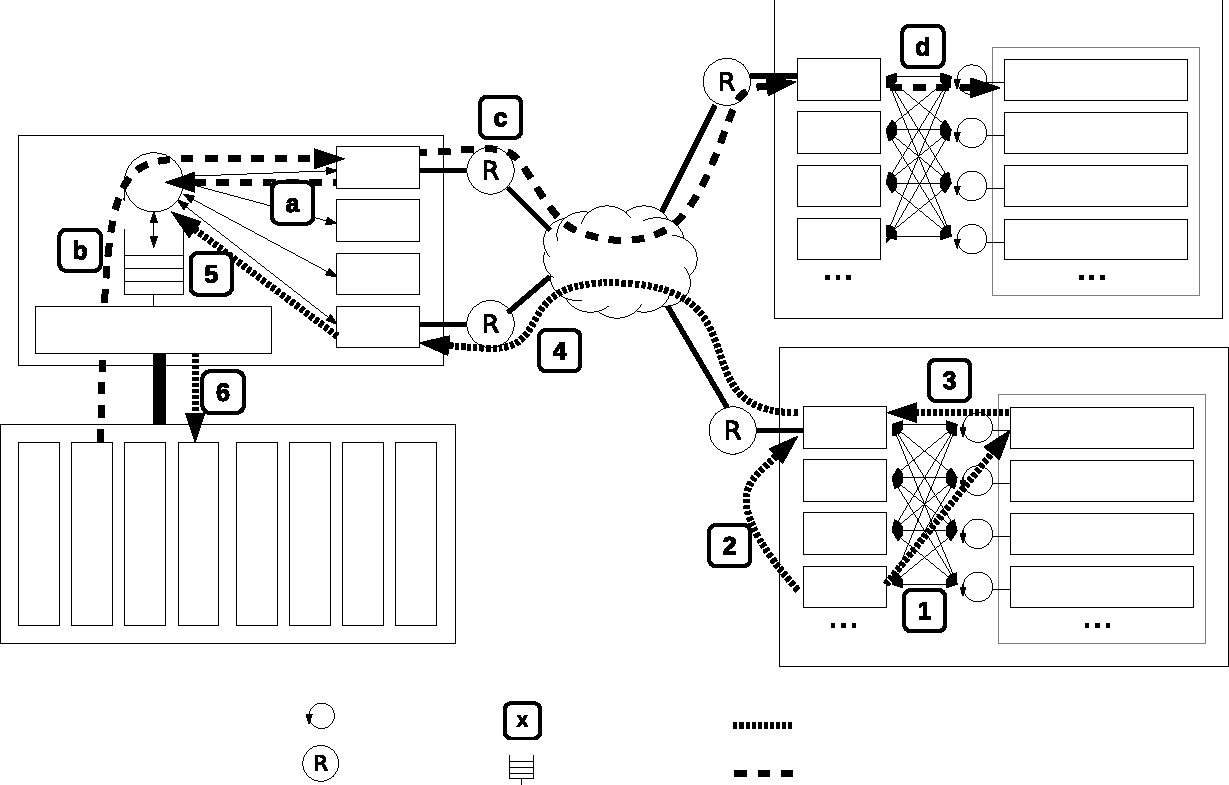
\includegraphics[width=15cm]{imgs/pdf/systemModel_MPPAremoteMem.pdf}}
		\put(371,65){\scriptsize Banc 4}
		\put(371,83){\scriptsize Banc 3}
		\put(371,102){\scriptsize Banc 2}
		\put(371,120){\scriptsize Banc 1}
		\put(368,186){\scriptsize Banc 4}
		\put(368,204){\scriptsize Banc 3}
		\put(368,223){\scriptsize Banc 2}
		\put(368,241){\scriptsize Banc 1}
		\put(355,140){\footnotesize SRAM Locale}
		\put(355,260){\footnotesize SRAM Locale}
		\put(429,146){\rotatebox{270}{\footnotesize Cluster B}}
		\put(427,267){\rotatebox{270}{\footnotesize Cluster A}}
		\put(282,65){\scriptsize C\oe{}ur 3}
		\put(282,83){\scriptsize C\oe{}ur 2}
		\put(282,102){\scriptsize C\oe{}ur 1}
		\put(284,120){\scriptsize DMA}
		\put(279,186){\scriptsize C\oe{}ur 3}
		\put(279,204){\scriptsize C\oe{}ur 2}
		\put(279,223){\scriptsize C\oe{}ur 1}
		\put(282,241){\scriptsize DMA}
		\put(206,179){\footnotesize NoC}
		\put(119,211){\scriptsize DMA 1}
		\put(120,193){\scriptsize C\oe{}ur 2}
		\put(120,175){\scriptsize C\oe{}ur 1}
		\put(119,156){\scriptsize DMA 2}
		\put(23,155){\footnotesize Contrôleur DDR}
		\put(95,127){\footnotesize DDR-SDRAM}
		\put(100,227){\footnotesize Cluster IO}
		\put(10,75){\rotatebox{90}{\scriptsize Banc 1}}
		\put(30,75){\rotatebox{90}{\scriptsize Banc 2}}
		\put(48,75){\rotatebox{90}{\scriptsize Banc 3}}
		\put(66,75){\rotatebox{90}{\scriptsize Banc 4}}
		\put(86,75){\rotatebox{90}{\scriptsize Banc 5}}
		\put(104,75){\rotatebox{90}{\scriptsize Banc 6}}
		\put(123,75){\rotatebox{90}{\scriptsize Banc 7}}
		\put(141,75){\rotatebox{90}{\scriptsize Banc 8}}
		\put(122,21){\footnotesize Arbitre}
		\put(122,5){\footnotesize Routeur Noc}
		\put(194,20){\footnotesize Étape}
		\put(194,5){\footnotesize File d'attente}
		\put(282,18){\footnotesize Procédure d'écriture}
		\put(282,4){\footnotesize Procédure de lecture}
	\end{picture}

	\caption{Exemple d'accès mémoires distants sur le \mppalong}
	\label{resumeFr_MPPAremoteMem}
\end{center}
\end{figure}
La procédure de lecture depuis la DDR-SDRAM s'effectue de manière relativement symétrique à celle d'écriture, à la différence qu'un RM sur un cluster IO doit être à l'initiative. Celui-ci peut lancer la procédure soit en réponse à une requête préalablement envoyée depuis un cluster de calcul soit en suivant les directives qui lui ont été imposées au travers d'une table d'ordonnancement.

En prenant l'exemple des procédures d'accès à la DDR-SDRAM, nous avons pu identifier les trois niveaux de ressources impliquant une corrélation entre les temps d'exécution d'applications concurrentes. Pour éliminer cette corrélation et permettre l'exécution des applications indépendamment les unes des autres, nous proposons de contraindre l'accès à ces trois ressources (la SRAM locale, le NoC et la DDR-SDRAM) par le biais d'un modèle d'exécution que nous détaillons et motivons dans la section suivante.


%\subsection{Modèles d'accès aux ressources partagées}
%\subsubsection{La SRAM locale}
%\subsubsection{Traversée du NoC}
%\subsubsection{Durée des requêtes vers la DDR-SDRAM}

\subsection{Réduction des interférences}
\label{ssec_resumeFr_reducInterference}
Afin d'éliminer les interférences non-désirées entre applications concurrentes, nous proposons d'utiliser un modèle d'exécution contraignant l'accès aux bancs de mémoire SRAM, au NoC et à la DDR-SDRAM. Ce modèle d'exécution est composé de 4 règles qui, si elles sont respectées (et nous verrons par la suite comment s'en assurer), permettent de partitionner le \mppalong en plusieurs environnements d'exécution indépendants les uns des autres. Nous définissons ainsi la notion de \emph{partition} comme suit:

\begin{defFr}[Partition]
    Une partition est un environnement d'exécution au sein duquel le comportement temporel d'une application ne dépend pas du comportement des applications appartenant à d'autres partitions.
\end{defFr}

Notre modèle d'exécution impose aux applications d'accéder aux ressources partagées tout en respectant 4 règles.

\begin{regleem}
    \label{em_resumeFr_regle1}
    Tout PE (et respectivement tout banc de SRAM locale) ne peut pas être réservé par plus d'une partition.
\end{regleem}

Grâce à la règle 1, nous assurons qu'un PE accèdant à un banc de SRAM locale ne subira pas d'interférences causées par des PEs d'autres partitions. Ainsi, les seules interférences à prendre en compte lors de l'accès à la SRAM sont celles provenant du trafic \emph{ami}, c'est-à-dire celui des autres PEs alloués à la partition. De ce fait, le calcul des WCETs peut non seulement être effectué de manière plus efficace en évitant de prendre en compte les pénalités d'interférence maximale (c'est-à-dire lorsque tous les PEs accèdent simultanément au même banc) mais cela permet également d'apporter une isolation temporelle entre les partitions. Le trafic initié par le RM et/ou le DMA peut toujours entrer en conflit avec celui des PEs d'une partition. Dans notre approche, nous prendrons l'hypothèse (que nous vérifierons par la suite) que ce trafic du RM ou du DMA dans un banc alloué à une partition n'est lié qu'au travail effectué dans cette partition et ne viole donc pas l'isolation temporelle. La Figure~\ref{fig_resumeFr_exampleRule1} représente un exemple d'application de cette règle sur un cluster de calcul simplifié et partagé par deux partitions. Ici, le choix de découpage a été fait équitablement (2 c\oe{}urs et 2 bancs par partition) mais n'importe quel autre découpage aurait été possible (3 c\oe{}urs et 1 banc pour l'une, 1 c\oe{}ur et 3 bancs pour l'autre, ...).
\begin{figure}
    \centering
    \begin{subfigure}[b]{0.45\linewidth}
    \centering
        \scalebox{0.7}{

% 1 : x; 2: y; 3: tikz object name
\newcommand\smemRRarb[3]{
    \node[circle, draw, color=black, anchor=south, thick, minimum size=1cm, inner sep=0pt] (#3) at (#1, #2) {A};
    \draw[ultra thick, ->, >=latex] (#3.west) -- ([yshift=-0.6em]#3.west); 
}

% X, Y, PRINTNAME, tikzlabel
\newcommand\smemCore[4]{
    \node[rectangle, draw, color=black, thick, anchor=south west, minimum width=2cm, minimum height=1cm, inner sep=0pt] (#4) at (#1, #2) {#3};
}

% X, Y, PRINTNAME, tikzlabel
\newcommand\smemBank[4]{
    \node[rectangle, draw, color=black, thick, anchor=south west, minimum width=2.5cm, minimum height=1cm, inner sep=0pt] (#4) at (#1, #2) {\emph{#3}};
    \smemRRarb{#1-1}{#2}{arb#4}
    \draw[thick] (arb#4.east) -- (#4.west);
}


\begin{tikzpicture}[font={\fontsize{12pt}{12}\selectfont}]

    \smemCore{0}{-6}{RM}{rm}
    \smemCore{0}{1.5}{DMA}{dma}
    
    \smemCore{0}{0}{PE 0}{pe0}
    \smemBank{6}{0}{Banc 0}{bank0}
        
    \smemCore{0}{-1.5}{PE 1}{pe1}
    \smemBank{6}{-1.5}{Banc 1}{bank1}
    
    \smemCore{0}{-3}{PE 2}{pe2}
    \smemBank{6}{-3}{Banc 2}{bank2}
    
    \smemCore{0}{-4.5}{PE 3}{pe3}
    \smemBank{6}{-4.5}{Banc 3}{bank3}

    \draw[thick] (pe0.east) -- (arbbank0.west);
    \draw[thick] (pe0.east) -- (arbbank1.west);
    \draw[thick] (pe0.east) -- (arbbank2.west);
    \draw[thick] (pe0.east) -- (arbbank3.west);

    \draw[thick] (pe1.east) -- (arbbank0.west);
    \draw[thick] (pe1.east) -- (arbbank1.west);
    \draw[thick] (pe1.east) -- (arbbank2.west);
    \draw[thick] (pe1.east) -- (arbbank3.west);

    \draw[thick] (pe2.east) -- (arbbank0.west);
    \draw[thick] (pe2.east) -- (arbbank1.west);
    \draw[thick] (pe2.east) -- (arbbank2.west);
    \draw[thick] (pe2.east) -- (arbbank3.west);

    \draw[thick] (pe3.east) -- (arbbank0.west);
    \draw[thick] (pe3.east) -- (arbbank1.west);
    \draw[thick] (pe3.east) -- (arbbank2.west);
    \draw[thick] (pe3.east) -- (arbbank3.west);

    \draw[thick, densely dotted] (dma.east) -- (arbbank0.west);
    \draw[thick, densely dotted] (dma.east) -- (arbbank1.west);
    \draw[thick, densely dotted] (dma.east) -- (arbbank2.west);
    \draw[thick, densely dotted] (dma.east) -- (arbbank3.west);
    
    \draw[thick, densely dotted] (rm.east) -- (arbbank0.west);
    \draw[thick, densely dotted] (rm.east) -- (arbbank1.west);
    \draw[thick, densely dotted] (rm.east) -- (arbbank2.west);
    \draw[thick, densely dotted] (rm.east) -- (arbbank3.west);

\end{tikzpicture}
}
        \caption{Sans la règle 1}
        \label{fig_resumeFr_exampleRule1_before}
    \end{subfigure}
    \begin{subfigure}[b]{0.45\linewidth}
    \centering
        \scalebox{0.7}{

% 1 : x; 2: y; 3: tikz object name
\newcommand\smemRRarb[3]{
    \node[circle, draw, color=black, anchor=south, thick, minimum size=1cm, inner sep=0pt] (#3) at (#1, #2) {A};
    \draw[ultra thick, ->, >=latex] (#3.west) -- ([yshift=-0.6em]#3.west); 
}

% X, Y, PRINTNAME, tikzlabel
\newcommand\smemCore[4]{
    \node[rectangle, draw, color=black, thick, anchor=south west, minimum width=2cm, minimum height=1cm, inner sep=0pt] (#4) at (#1, #2) {#3};
}

% X, Y, PRINTNAME, tikzlabel
\newcommand\smemBank[4]{
    \node[rectangle, draw, color=black, thick, anchor=south west, minimum width=2.5cm, minimum height=1cm, inner sep=0pt] (#4) at (#1, #2) {\emph{#3}};
    \smemRRarb{#1-1}{#2}{arb#4}
    \draw[thick] (arb#4.east) -- (#4.west);
}


\begin{tikzpicture}[font={\fontsize{12pt}{12}\selectfont}]

    \smemCore{0}{-6}{RM}{rm}
    \smemCore{0}{1.5}{DMA}{dma}
    
    \smemCore{0}{0}{PE 0}{pe0}
    \smemBank{6}{0}{Banc 0}{bank0}
        
    \smemCore{0}{-1.5}{PE 1}{pe1}
    \smemBank{6}{-1.5}{Banc 1}{bank1}
    
    \smemCore{0}{-3}{PE 2}{pe2}
    \smemBank{6}{-3}{Banc 2}{bank2}
    
    \smemCore{0}{-4.5}{PE 3}{pe3}
    \smemBank{6}{-4.5}{Banc 3}{bank3}

    \draw[thick] (pe0.east) -- (arbbank0.west);
    \draw[thick] (pe0.east) -- (arbbank1.west);

    \draw[thick] (pe1.east) -- (arbbank0.west);
    \draw[thick] (pe1.east) -- (arbbank1.west);

    \draw[thick] (pe2.east) -- (arbbank2.west);
    \draw[thick] (pe2.east) -- (arbbank3.west);

    \draw[thick] (pe3.east) -- (arbbank2.west);
    \draw[thick] (pe3.east) -- (arbbank3.west);

    \draw[thick, densely dotted] (dma.east) -- (arbbank0.west);
    \draw[thick, densely dotted] (dma.east) -- (arbbank1.west);
    \draw[thick, densely dotted] (dma.east) -- (arbbank2.west);
    \draw[thick, densely dotted] (dma.east) -- (arbbank3.west);
    
    \draw[thick, densely dotted] (rm.east) -- (arbbank0.west);
    \draw[thick, densely dotted] (rm.east) -- (arbbank1.west);
    \draw[thick, densely dotted] (rm.east) -- (arbbank2.west);
    \draw[thick, densely dotted] (rm.east) -- (arbbank3.west);

    \node[rectangle, draw, color=black, thick, dashed, anchor=south west, minimum width=8.8cm, minimum height=2.8cm, inner sep=0pt] at (-0.15, -1.65) { };
    \node[minimum width=2.5cm, anchor=south west] at (6,1.3) {\Large Part. 1};

    \node[rectangle, draw, color=black, thick, dashed, anchor=south west, minimum width=8.8cm, minimum height=2.8cm, inner sep=0pt] at (-0.15, -4.65) { };
    \node[minimum width=2.5cm, anchor=north west] at (6,-4.8) {\Large Part. 2};

\end{tikzpicture}
}
        \caption{Avec la règle 1}
        \label{fig_resumeFrl_exampleRule1_after}
    \end{subfigure}
    \caption{Exemple d'application de la règle 1 du modèle d'exécution sur une architecture simplifiée de cluster de calcul avec 2 partitions}
    \label{fig_resumeFr_exampleRule1}
\end{figure}





\begin{regleem}
    \label{em_resumeFr_regle2}
    Les communications sur le NoC doivent respecter un ordonnancement global dirigé par le temps et éviter les conflits en utilisant soit des routes différentes soit en accédant aux ressources à des instants différents. L'ordonnancement du NoC doit garantir que, lorsque une route est utilisée par une communication, elle lui est complètement réservée pour sa durée d'utilisation.
\end{regleem}

Un ordonnancement dirigé par le temps permet de largement simplifier le calcul des temps de traversée maximaux des paquets envoyés. En effet, en ne considérant aucun conflit d'accès aux ressources NoC, les pires temps de traversée peuvent être déduits efficacement de modèles matériels simples. En revanche, ce bénéfice n'est possible qu'au détriment de la flexibilité de l'approche et au coût d'efforts supplémentaires lors du pré-calcul de l'ordonnancement pour éviter les conflits par construction. Les travaux précédents visant à rendre le NoC du \mppalong prédictible utilisent généralement une approche asynchrone en utilisant les régulateurs d'injection matériels des interfaces NoC. Dans \cite{Dinechin2014} ou \cite{Giannopoulou2015}, les auteurs configurent par exemple ces régulateurs d'injection en appliquant la théorie du Calcul Réseau~\cite{LeBoudec2001, Cruz91}. Si ces approches sont généralement reconnues comme apportant une certaine flexibilité et des garanties sûres et peu pessimistes sur les \emph{bandes passantes} allouées aux applications, notre choix d'un ordonnancement global dirigé par le temps s'explique par deux raisons:
\begin{enumerate}
    \item Notre objectif principal est d'apporter une garantie d'isolation temporelle stricte entre les partitions. Les approches asynchrones utilisant le calcul réseau permettent de borner de manière sûre les interférences sur le NoC mais n'évitent pas les conflits. Ainsi, le temps de traversée d'un paquet dans le cas asynchrone est, même si cela peut être borné, dépendant de l'utilisation qui est faite du NoC par les partitions concurrentes. Pour obtenir une isolation temporelle stricte, l'évitement complet des conflits par un ordonnancement global apparaît alors plus adapté.
    \item Un des objectifs sous-jacents à notre approche est de permettre l'exploitation efficace du \mppalong avec des applications distribuées sur plusieurs clusters. Ainsi, notre capacité à garantir des \emph{latences} courtes pour l'échange de messages entre les clusters est un point particulièrement important. Il a été montré dans~\cite{Puffitsch2015} qu'un ordonnancement global dirigé par le temps permet de satisfaire ce type de contraintes là où des approches asynchrones basées sur le calcul réseau permettent plutôt d'obtenir des garanties efficaces sur les \emph{bandes passantes}.
\end{enumerate}

\begin{figure}
    \centering
    \begin{subfigure}[b]{0.4\linewidth}
    \centering
        \scalebox{0.7}{
% 1 : x; 2: y; 3: tikz object name
\newcommand\nocnode[3]{
    \node[circle, draw, color=black, anchor=south, thick, minimum size=1cm, inner sep=0pt] (r#3) at (#1, #2) {#3};
}

\begin{tikzpicture}[font={\fontsize{12pt}{12}\selectfont}]
    
    \nocnode{0}{0}{1}
    \nocnode{3}{0}{2}
    \nocnode{6}{0}{3}
    \nocnode{0}{-2.5}{4}
    \nocnode{3}{-2.5}{5}
    \nocnode{6}{-2.5}{6}

    \draw[-latex, thick, loosely dashed] (r1) -- (r2);
    \draw[-latex, thick, loosely dashed] (r2.230) -- (r5.130);
    \draw[-latex, thick, loosely dashed] (r5) -- (r6);

    \draw[-latex, thick, densely dotted] (r3) -- (r2);
    \draw[-latex, thick, densely dotted] (r2.310) -- (r5.50);
    \draw[-latex, thick, densely dotted] (r5) -- (r4);

\end{tikzpicture}
}
        \caption{NoC Simplifié}
        \label{fig_resumeFr_exampleRule2_noc}
    \end{subfigure}
    \begin{subfigure}[b]{0.59\linewidth}
    \centering
        \tikzset{timing/.append style={x=1.8ex, y=3ex}}
        

\begin{tikztimingtable}[timing/lslope=0, timing/slope=0, timing/coldist=0.5, timing/d/text/.append style={font=\rmfamily}, timing/d/background/.style={fill=gray}]
    $1 \to 6$ & L 3D 6L 3D 6L \\     
    $3 \to 4$ & 5L 2D 7L 2D 3L \\     
\extracode
\begin{background}
    \vertlines[dashed]{}
\end{background}
\end{tikztimingtable}



        \caption{Ordonnancement des communications}
        \label{fig_resumeFr_exampleRule2_diagram}
    \end{subfigure}
    \caption{Exemple d'application de la règle 2 du modèle d'exécution avec 2 communications partageant un lien NoC \circled{2} $\to$ \circled{5}}
    \label{fig_resumeFr_exampleRule2}
\end{figure}

La Figure~\ref{fig_resumeFr_exampleRule2} représente un exemple d'application de la règle 2 du modèle d'exécution sur un NoC simplifié pour lequel une ressource est partagée par deux communications. Le conflit d'accès à cette ressource est alors résolu par l'allocation de créneaux d'accès périodiques à chaque communication en évitant leur recouvrement temporel.





\begin{regleem}
    \label{em_resumeFr_regle3}
    Toutes les zones mémoires qu'une application souhaite envoyer au travers du NoC doivent être intégralement définies hors-ligne.
\end{regleem}

L'application de la règle 3 n'est pas absolument nécessaire pour garantir une isolation temporelle entre partitions. Cependant, elle apporte plusieurs propriétés intéressantes pour l'implémentation. En connaissant à l'avance les zones mémoire qui seront envoyées au travers des créneaux alloués aux communications, il devient possible de vérifier hors-ligne que la taille de ces créneaux est suffisante pour permettre l'envoi des données. En particulier, il possible de vérifier en utilisant des modèles du matériel relativement simples (sachant que l'on prend l'hypothèse que les conflits sont évités par construction) que le temps alloué à l'envoi d'une donnée est suffisant pour permettre sa traversée complète du NoC. Par ailleurs, cette règle simplifie considérablement l'implémentation de notre \emph{hyperviseur} et permet notamment de réduire son WCET qui, comme nous le montrerons par la suite, est un critère majeur pour obtenir de bonnes performances. Enfin, connaître à priori les zones mémoires visées par le DMA (notamment en réception) est un atout pour calculer efficacement les pénalités d'interférence subies par les PEs en accédant à leurs bancs de SRAM locale.







\begin{regleem}
    \label{em_resumeFr_regle4}
    Un banc de DDR-SDRAM externe peut être partagé par plusieurs partitions si et seulement si elles n'y accèdent jamais simultanément.
\end{regleem}

L'application de la règle 4 permet d'éviter les conflits d'accès entre plusieurs masters accédant à différentes lignes d'un même banc de DDR-SDRAM. En effet, les lectures et écritures en DDR-SDRAM ne peuvent s'effectuer qu'après l'ouverture préalable par le contrôleur de la ligne adéquate dans le banc visé. Dans le cas où deux masters initieraient des transactions visant des zones différentes d'un même banc simultanément, il serait nécessaire pour borner la durée de ces transactions de considérer les fermetures de lignes intempestives dues aux accès concurrents. En évitant ce problème par construction, on peut tirer parti du parallélisme de la DDR-SDRAM banquée tout en garantissant une bonne prédictibilité. En revanche, cela implique une difficulté supplémentaire lors du pré-calcul de l'ordonnancement des accès à la mémoire.

\begin{figure}
    \centering
    \begin{subfigure}[b]{0.3\linewidth}
    \centering
        \scalebox{0.6}{
% 1 : x; 2: y; 3: tikz object name; 4: printname
\newcommand\partnode[4]{
    %\node[circle, draw, color=black, thick, minimum size=1cm, inner sep=0pt] (#3) at (#1, #2) {#4};
    \node[rectangle, draw, rounded corners, color=black, thick, minimum width=1cm, minimum height=1cm, inner sep=0pt] (#3) at (#1, #2) {#4};
}

\begin{tikzpicture}[font={\fontsize{12pt}{12}\selectfont}]
    
    \node[circle, draw, color=black, thick, minimum size=1.3cm, inner sep=0pt] (arb) at (0, 0) {Arb.};
    \draw[ultra thick, ->, >=latex] (arb.west) -- ([yshift=-0.6em]arb.west); 
   
    \partnode{-2}{-1.2}{A}{$P_A$}
    \partnode{0}{-1.6}{B}{$P_B$}
    \partnode{2}{-1.2}{C}{$P_C$}

    \draw[-latex, thick] (A) -- (arb);
    \draw[-latex, thick] (B) -- (arb);
    \draw[-latex, thick] (C) -- (arb);
    
    \node[rectangle, draw, color=black, thick, dashed, anchor=south west, minimum width=7.4cm, minimum height=3cm] (ddrmodule) at (-3.7, 1.2) {};
    \node[anchor=north west, minimum height=0.5cm] at (-3.7, 1.2) {\emph{\small DDR-SDRAM}};
    \draw[-latex, thick] (arb.north) -- (ddrmodule.south);

    \node[anchor=north west, minimum width=1cm, minimum height=0.7cm, ] at (-3.5, 2) {$b_0$};
    \node[rectangle, draw, color=black, pattern=north east lines, thick, anchor=south west, minimum width=1cm, minimum height=2cm, ] at (-3.5, 2) {}; %B0
    
    \node[anchor=north west, minimum width=1cm, minimum height=0.7cm, ] at (-2.3, 2) {$b_1$};
    \node[rectangle, draw, color=black, pattern=north east lines, thick, anchor=south west, minimum width=1cm, minimum height=2cm] at (-2.3, 2) {}; %B1
    
    \node[anchor=north west, minimum width=1cm, minimum height=0.7cm, ] at (-1.1, 2) {$b_2$};
    \node[rectangle, draw, color=black, pattern=north east lines, thick, anchor=south west, minimum width=1cm, minimum height=0.6cm] at (-1.1, 2) {}; %B2
    \node[rectangle, draw, color=black, pattern=dots, thick, anchor=south west, minimum width=1cm, minimum height=1.4cm] at (-1.1, 2.6) {}; %B2
    
    \node[anchor=north west, minimum width=1cm, minimum height=0.7cm, ] at (0.1, 2) {$b_3$};
    \node[rectangle, draw, color=black, pattern=dots, thick, anchor=south west, minimum width=1cm, minimum height=1.3cm] at (0.1, 2) {}; %B3
    \node[rectangle, draw, color=black, pattern=grid, thick, anchor=south west, minimum width=1cm, minimum height=0.7cm] at (0.1, 3.3) {}; %B3
    
    \node[anchor=north west, minimum width=1cm, minimum height=0.7cm, ] at (1.3, 2) {$b_4$};
    \node[rectangle, draw, color=black, pattern=grid, thick, anchor=south west, minimum width=1cm, minimum height=2cm] at (1.3, 2) {}; %B4
    
    \node[anchor=north west, minimum width=1cm, minimum height=0.7cm, ] at (2.5, 2) {$b_5$};
    \node[rectangle, draw, color=black, pattern=grid, thick, anchor=south west, minimum width=1cm, minimum height=2cm] at (2.5, 2) {}; %B5

    
    \node (noteA) at (-4,3.5) {$P_A$};
    \draw (noteA) -- (-3,3);

    \node (noteB) at (-1,4.5) {$P_B$};
    \draw (noteB) -- (-0.5,3.5);

    \node (noteC) at (2.5,4.5) {$P_C$};
    \draw (noteC) -- (2,3.5);
\end{tikzpicture}
}
        \caption{Accès à la DDR-SDRAM}
        \label{fig_resumeFr_exampleRule4_ddr}
    \end{subfigure}\hspace{6mm}
    \begin{subfigure}[b]{0.65\linewidth}
    \centering
        \tikzset{timing/.append style={x=2.2ex, y=3ex}}
        

\begin{tikztimingtable}[timing/lslope=0, timing/slope=0, timing/coldist=0.5, timing/d/text/.append style={font=\rmfamily}, timing/d/background/.style={fill=gray}]
    $P_A$ & L 3D 7L 3D 5L \\     
    $P_B$ & 5L D 9L D 3L \\     
    $P_C$ & 2L 1.5D 3.5L 1.5D 3.5L 1.5D 3.5L 1.5D 0.5L \\     
\extracode
\begin{background}
    \vertlines[dashed]{}
\end{background}
\end{tikztimingtable}



        \caption{Ordonnancement des accès à la DDR-SDRAM}
        \label{fig_resume_exampleRule4_diagram}
    \end{subfigure}
    \caption{Exemple d'application de la règle 4 du modèle d'exécution sur un arbitre DDR-SDRAM simplifié et 3 masters $P_A$, $P_B$ et $P_C$ en concurrence pour accéder à la mémoire}
    \label{fig_resumeFr_exampleRule4}
\end{figure}

La Figure~\ref{fig_resumeFr_exampleRule4} représente un exemple d'application de la règle 4 dans une situation où 3 partitions ($P_A$, $P_B$ et $P_C$) accèdent à une DDR-SDRAM qui comporte des bancs partagés. Dans ce cas, les accès issus des partitions en situation de partage sont ordonnancés de façon à éviter le recouvrement temporel, et donc le cas où deux partitions accèderaient à des zones différentes d'un banc en même temps. En outre, les partitions ne partageant pas de bancs ($P_A$ et $P_C$ dans cet exemple) sont quant à elles autorisées à accéder simultanément à la DDR-SDRAM.



\subsection{Synthèse}
Dans cette section, nous avons identifié la SRAM locale, le NoC et la DDR-SDRAM comme les trois ressources impliquant une corrélation entre les temps d'exécution des programmes concurrents non contrôlés sur le \mppalong. Dans un contexte où nous voudrions exécuter des applications dans des environnements d'exécution temporellement isolés les uns des autres, nous avons défini une notion de partition qui capture la problématique de l'isolation temporelle. Sur cette base, nous avons défini un modèle d'exécution permettant d'éliminer les interférences subies par les applications lorsque elles accèdent aux ressources partagées. Ce modèle d'exécution repose sur un partitionnement purement spatial au sein des clusters de calcul et sur un partitionnement spatialo-temporel pour le NoC et la DDR-SDRAM. De manière générale, notre approche s'appuie sur une pré-réservation des ressources matérielles du processeur. Dans la section suivante, nous formaliserons une notion de \emph{budget de partition} qui représente cette pré-réservation et nous montrerons comment elle peut être utilisée dans le cadre d'un processus d'intégration automatisé.





\section{Atelier d'intégration}
\label{sec_resumeFr_workflow}

Dans cette section, nous présentons un atelier permettant l'intégration de plusieurs applications temporellement isolées les unes des autres sur le \mppalong. Cet atelier repose principalement sur la propriété d'isolation temporelle apportée par notre modèle d'exécution. Comme cela est décrit sur la Figure~\ref{fig_resumeFr_workFlow}, plusieurs étapes sont nécessaires à l'intégration de partitions à partir de modèles hauts niveaux des applications jusqu'à une exécution concurrente sur la cible de façon prédictible. D'une manière générale, l'atelier repose sur un ensemble de calculs hors-ligne permettant la génération de tables d'ordonnancement qui seront appliquées en-ligne. Nous détaillons d'abord les entrées de cet atelier et formalisons notamment la notion de \emph{budget de ressource} avant de décrire les objectifs des différentes étapes de pré-calcul et d'introduire le support logiciel nécessaire en-ligne garantissant le respect du modèle d'exécution.


\begin{figure}
    \centering
    \scalebox{0.9}{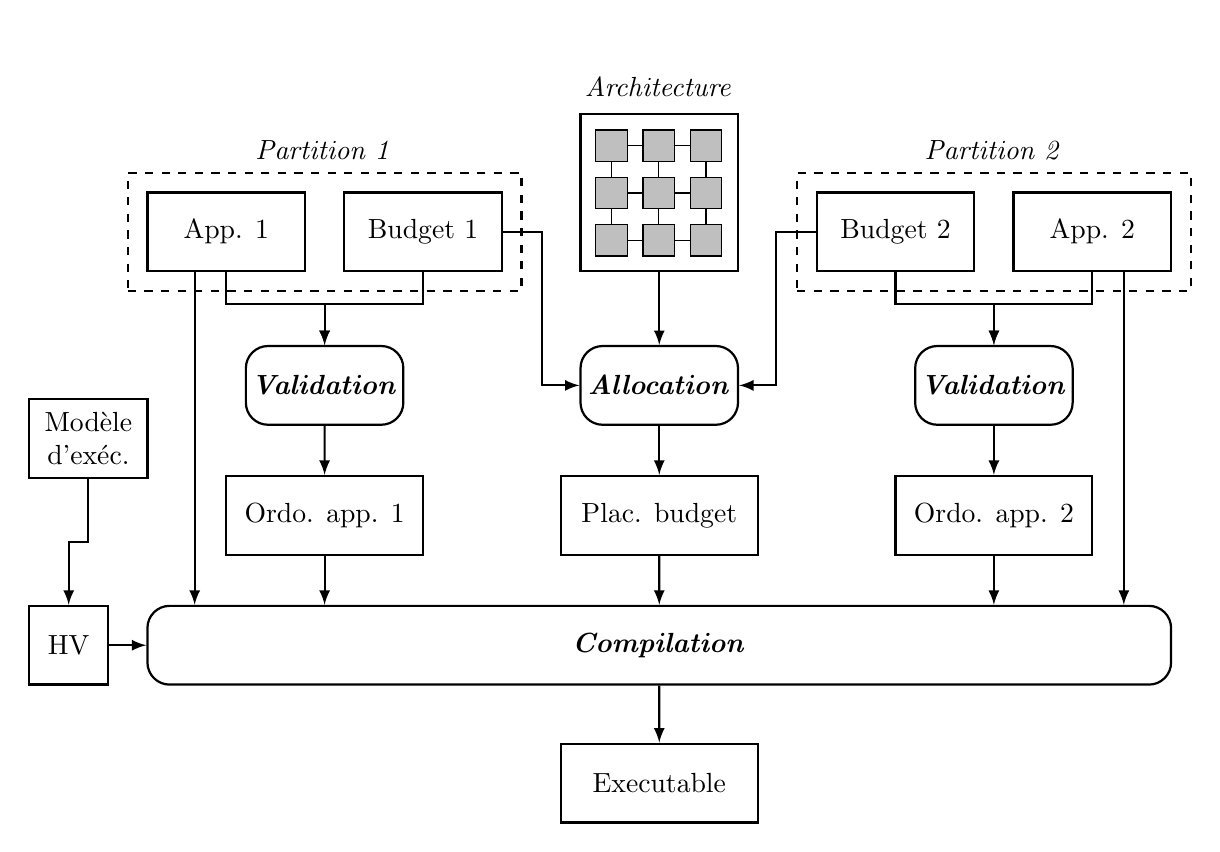
\begin{tikzpicture}
\draw (5.5,0) node[draw, rectangle, inner sep=0pt, minimum width=2cm, minimum height=2cm, anchor=south west, thick] (Archi) {};
\draw (5.7,0.2) node[draw, rectangle, inner sep=0pt, minimum width=0.4cm, minimum height=0.4cm, anchor=south west, fill=lightgray] (t11) {};
\draw (6.3,0.2) node[draw, rectangle, inner sep=0pt, minimum width=0.4cm, minimum height=0.4cm, anchor=south west, fill=lightgray] (t12) {};
\draw (6.9,0.2) node[draw, rectangle, inner sep=0pt, minimum width=0.4cm, minimum height=0.4cm, anchor=south west, fill=lightgray] (t13) {};
\draw (5.7,0.8) node[draw, rectangle, inner sep=0pt, minimum width=0.4cm, minimum height=0.4cm, anchor=south west, fill=lightgray] (t21) {};
\draw (6.3,0.8) node[draw, rectangle, inner sep=0pt, minimum width=0.4cm, minimum height=0.4cm, anchor=south west, fill=lightgray] (t22) {};
\draw (6.9,0.8) node[draw, rectangle, inner sep=0pt, minimum width=0.4cm, minimum height=0.4cm, anchor=south west, fill=lightgray] (t23) {};
\draw (5.7,1.4) node[draw, rectangle, inner sep=0pt, minimum width=0.4cm, minimum height=0.4cm, anchor=south west, fill=lightgray] (t31) {};
\draw (6.3,1.4) node[draw, rectangle, inner sep=0pt, minimum width=0.4cm, minimum height=0.4cm, anchor=south west, fill=lightgray] (t32) {};
\draw (6.9,1.4) node[draw, rectangle, inner sep=0pt, minimum width=0.4cm, minimum height=0.4cm, anchor=south west, fill=lightgray] (t33) {};
\draw (t11) -- (t12) -- (t13); 
\draw (t21) -- (t22) -- (t23); 
\draw (t31) -- (t32) -- (t33); 
\draw (t11) -- (t21) -- (t31); 
\draw (t12) -- (t22) -- (t32); 
\draw (t13) -- (t23) -- (t33); 

\draw (5.5,1.6) node[inner sep=0pt, minimum width=2cm, minimum height=1.5cm, anchor=south west] {\textit{Architecture}};

\draw (0,0) node[draw, rectangle, inner sep=0pt, minimum width=2cm, minimum height=1cm, anchor=south west, thick] (App1) {App. 1};
\draw (2.5,0) node[draw, rectangle, inner sep=0pt, minimum width=2cm, minimum height=1cm, anchor=south west, thick] (Bud1) {Budget 1};
\draw (8.5,0) node[draw, rectangle, inner sep=0pt, minimum width=2cm, minimum height=1cm, anchor=south west, thick] (Bud2) {Budget 2};
\draw (11,0) node[draw, rectangle, inner sep=0pt, minimum width=2cm, minimum height=1cm, anchor=south west, thick] (App2) {App. 2};

\draw (-0.25,-0.25) node[draw, rectangle, inner sep=0pt, minimum width=5cm, minimum height=1.5cm, anchor=south west, thick, dashed] {};
\draw (-0.25,0.8) node[inner sep=0pt, minimum width=5cm, minimum height=1.5cm, anchor=south west] {\textit{Partition 1}};
\draw (8.25,-0.25) node[draw, rectangle, inner sep=0pt, minimum width=5cm, minimum height=1.5cm, anchor=south west, thick, dashed] {};
\draw (8.25,0.8) node[inner sep=0pt, minimum width=5cm, minimum height=1.5cm, anchor=south west] {\textit{Partition 2}};

\draw (5.5,-1.95) node[draw, rectangle, inner sep=0pt, minimum width=2cm, minimum height=1cm, anchor=south west, rounded corners=8pt, thick] (Alloc) { \textbf{\textit{Allocation}}};
\draw (1.25,-1.95) node[draw, rectangle, inner sep=0pt, minimum width=2cm, minimum height=1cm, anchor=south west, rounded corners=8pt, thick] (Valid1) {\textbf{\textit{Validation}}};
\draw (9.75,-1.95) node[draw, rectangle, inner sep=0pt, minimum width=2cm, minimum height=1cm, anchor=south west, rounded corners=8pt, thick] (Valid2) {\textbf{\textit{Validation}}};

\draw[-latex, thick] (App1.south) -- ([yshift=-4mm]App1.south) -| (Valid1.north);
\draw[-latex, thick] (Bud1.south) -- ([yshift=-4mm]Bud1.south) -| (Valid1.north);
\draw[-latex, thick] (App2.south) -- ([yshift=-4mm]App2.south) -| (Valid2.north);
\draw[-latex, thick] (Bud2.south) -- ([yshift=-4mm]Bud2.south) -| (Valid2.north);
\draw[-latex, thick] (Bud1.east) -- ([xshift=5mm]Bud1.east) |- (Alloc.west);
\draw[-latex, thick] (Bud2.west) -- ([xshift=-5mm]Bud2.west) |- (Alloc.east);
\draw[-latex, thick] (Archi.south) --  (Alloc.north);

\draw (1,-3.6) node[draw, rectangle, inner sep=0pt, minimum width=2.5cm, minimum height=1cm, anchor=south west, thick] (AppMap1) {Ordo. app. 1};
\draw (5.25,-3.6) node[draw, rectangle, inner sep=0pt, minimum width=2.5cm, minimum height=1cm, anchor=south west, thick] (BudMap) {Plac. budget};
\draw (9.5,-3.6) node[draw, rectangle, inner sep=0pt, minimum width=2.5cm, minimum height=1cm, anchor=south west, thick] (AppMap2) {Ordo. app. 2};

\draw[-latex, thick] (Valid1.south) --  (AppMap1.north);
\draw[-latex, thick] (Valid2.south) --  (AppMap2.north);
\draw[-latex, thick] (Alloc.south) --  (BudMap.north);    

\draw (-1.5,-2.625) node[draw, rectangle, inner sep=0pt, minimum width=1.5cm, minimum height=1cm, anchor=south west, text width=1.25cm, align=center, thick] (EM) {Modèle \\ d'exéc.};

\draw (-1.5,-5.25) node[draw, rectangle, inner sep=0pt, minimum width=1cm, minimum height=1cm, anchor=south west, thick] (HV) {HV};

\draw[-latex, thick] (EM.south) -- ([yshift=-8mm]EM.south) -| (HV.north);

\draw (0,-5.25) node[draw, rectangle, inner sep=0pt, minimum width=13cm, minimum height=1cm, anchor=south west, rounded corners=8pt, thick] (Compile) {\textbf{\textit{Compilation}}};

\draw[-latex, thick] (AppMap1.south) --  (AppMap1|-Compile.north);
\draw[-latex, thick] (AppMap2.south) --  (AppMap2|-Compile.north);
\draw[-latex, thick] (BudMap.south) --  (Compile.north);
\draw[-latex, thick] ([xshift=-4mm]App1.south) --  ([xshift=-4mm]App1.south|-Compile.north);
\draw[-latex, thick] ([xshift=4mm]App2.south) --  ([xshift=4mm]App2.south|-Compile.north);
\draw[-latex, thick] (HV.east) --  (Compile.west);

\draw (5.25,-7) node[draw, rectangle, inner sep=0pt, minimum width=2.5cm, minimum height=1cm, anchor=south west, thick] (exec) {Executable};
\draw[-latex, thick] (Compile.south) --  (exec.north);


\end{tikzpicture}

}
    \caption{Atelier d'intégration de partitions multiples sur le \mppalong}
    \label{fig_resumeFr_workFlow}
\end{figure}



\subsection{Paramètres d'entrées}
\label{ssec_resumeFr_paramEntreeWorkflow}
Notre atelier d'intégration prend tout d'abord en entrée un modèle de l'architecture du \mppalong. Nous notons les éléments de ce modèle comme un quadruplet $< C_K , I_K , N_K, R_K >$ où:
\begin{itemize}
    \item $C_K = \{ c_K^0 , \ldots , c_K^{15} \}$ représentent les 16 clusters de calcul.
    \item $I_K = \{ i_K^0 , \ldots , i_K^{15} \}$ représentent les 16 RMs des clusters I/O.
    \item $N_K = \{ n_K^0 , \ldots , n_K^{31} \}$ représentent les 32 n\oe{}uds du NoC.
    \item $R_K = \bigcup R_K^{ij}$ est l'ensemble des chemins NoC avec $R_K^{ij}$ les chemins de $n_K^i$ à $n_K^j$.
\end{itemize}

L'autre type d'entrée de notre atelier est les partitions. Chaque application dans une partition est modélisée comme précédemment expliqué (Section~\ref{ssec_resumeFr_appModel}). En outre, chaque partition est associée à un \emph{budget de ressources} qui représente la quantité de ressources matérielles dont l'application a besoin pour s'exécuter correctement. Plus précisément le budget d'une partition $\mathcal{P}_i$ s'écrit comme un quadruplet $<\mathcal{N}_i , \mathcal{I}_i , \mathcal{C}_i , \mathcal{B}_i>$ où:

\begin{enumerate}
        \item  $\mathcal{N}_i = \{ pn_1^i , \ldots , pn_n^i \}$ est un ensemble fini de \emph{N\oe{}uds de Partition} (ou \emph{PNs}). Un PN représente un besoin en puissance de calcul à l'intérieur d'un cluster de calcul pour une partition. Un PN représente la réservation d'un nombre de PEs et d'un nombre de bancs de SRAM locale pour une partition. Plus formellement:
            \begin{itemize}
                \item $N_c : \mathcal{N}_i \mapsto \mathbb{N}$ associe chaque PN avec le nombre de PEs qui se doivent de lui être réservés dans un cluster de calcul.
                \item $N_b : \mathcal{N}_i \mapsto \mathbb{N}$ associe chaque PN avec le nombre de bancs de SRAM locale qui se doivent de lui être réservés dans un cluster de calcul.
            \end{itemize}

        \item $\mathcal{I}_i = \{ io_1^i , \ldots , io_o^i \}$ est un ensemble de \emph{N\oe{}uds I/O} (ou \emph{ION}s). Un ION est un point d'accès à la DDR-SDRAM externe matérialisé par un RM de cluster I/O. Son objectif est de répondre aux requêtes d'écritures et de lectures en DDR-SDRAM distantes initiées par les PNs.

        \item $\mathcal{C}_i = \{ pc_1^i , \ldots , pc_p^i \}$ est un ensemble de \emph{Communications de Partition} (ou \emph{PC}). Une PC est un canal de communication directionnel permettant l'échange de données entre PNs ou entre PNs et IONs. Une PC représente un créneau d'accès périodique au NoC sur un chemin donné. Plus formellement:
            \begin{itemize}
                \item $src : \mathcal{C}_i \mapsto \mathcal{N}_i \cup \mathcal{I}_i$ associe chaque PC avec son PN ou ION source.
                \item $dst : \mathcal{C}_i \mapsto \mathcal{N}_i \cup \mathcal{I}_i$ associe chaque PC avec son PN ou ION destination.
                \item $T : \mathcal{C}_i \mapsto \mathbb{N}$ fournit la \emph{période} d'activation du PC.
                \item $C : \mathcal{C}_i \mapsto \mathbb{N}$ fournit la \emph{durée} du créneau d'accès au NoC d'un PC.
                \item $O : \mathcal{C}_i \mapsto \mathbb{N}$ fournit l'\emph{offset} du \PC{}, aussi appelé la première date d'activation.
                \item $R : \mathcal{C}_i \mapsto \mathbb{N}$ fournit le plus grand nombre de n\oe{}uds du NoC qui peuvent être traversés par le chemin alloué au PC. Cela peut être utilisé afin d'imposer une contrainte sur la latence NoC maximale acceptable pour le PC en considération.

            \end{itemize}

        \item $\mathcal{B}$ représente un nombre de bancs de DDR-SDRAM externe.
    \end{enumerate}

De façon générale, une partition inclut une application ainsi qu'un budget de ressources \emph{abstraites} formalisées sous la notion de \emph{budget}. De ce fait, les développeurs d'applications peuvent exprimer leurs besoins en ressources matérielles tôt dans le processus de développement. Avec une telle approche fondée sur la pré-réservation de ressources, il est possible de concevoir, de développer, de tester et de qualifier une application sans nécessiter d'avoir connaissance des partitions concurrentes. En revanche, cela implique d'apporter un support hors-ligne et en-ligne du modèle d'exécution. Ces deux aspects sont développés dans les sections suivantes.


%\subsubsection{Modèle de la plateforme}
%\subsubsection{Budget de ressources}

\subsection{Calculs hors-ligne}
Comme cela est montré sur la Figure~\ref{fig_resumeFr_workFlow}, notre atelier de conception suppose deux étapes de calculs hors-ligne pour la \emph{Validation} et l'\emph{Allocation} des budgets. L'étape de Validation consiste à confirmer que le budget alloué à une application est effectivement suffisant pour qu'elle s'exécute de manière satisfaisante, c'est-à-dire en respectant l'ensemble de ses contraintes fonctionnelles et non-fonctionnelles. Plus précisément, nous recherchons lors de la Validation à déterminer un placement et un ordonnancement de l'application sur les ressources qui lui sont associées tout en respectant les contraintes applicatives telles que les précédences ou échéances des tâches et sous-tâches. L'automatisation de cette étape en utilisant la programmation par contraintes est l'objet de la Section~\ref{sec_resumeFr_validation}.

Lors de l'étape d'Allocation, les ressources \emph{abstraites} représentées par les PNs, IONs et PCs sont allouées à des ressources \emph{concrètes} de la cible matérielle. Par exemple, c'est lors de cette étape d'allocation que la décision de placer (ou non) deux PNs de deux partitions différentes sur le même cluster sera prise, compte tenu des ressources matérielles disponibles (16 PEs et 15 bancs de SRAM locale~\footnote{Le dernier banc de SRAM locale sera réservé pour le système dans notre approche. Cela est détaillé en Section~\ref{sec_resumeFr_hv}.} dans chaque cluster) et des ressources matérielles requises pour les PNs. En l'état d'avancement actuel, nous disposons d'une version préliminaire de l'implémentation automatique de l'étape d'Allocation qui, en utilisant la programmation par contraintes, semble fournir des résultats intéressants. Il apparaît toutefois qu'une série d'analyses et d'évaluations plus poussées sont nécessaires pour que celle-ci puisse être considérée comme mature. Ainsi, les travaux développés dans ce document se focaliseront sur l'étape de Validation, laissant l'automatisation de l'étape d'Allocation comme une perspective intéressante de travaux futurs. 

\subsection{Support d'exécution en-ligne}
Une fois les tâches, sous-tâches et données des applications placées et ordonnancées à l'intérieur de leurs budgets, et une fois les budgets des différentes partitions alloués à des ressources matérielles concrètes, il reste à garantir à l'exécution que les frontières entre partitions ne sont pas violées par les applications pour garantir leur isolation temporelle. Pour ce faire, nous proposons d'instancier notre modèle d'exécution au sein d'une couche basse de régulation logicielle appelée un \emph{hyperviseur}. Celui-ci sera en charge de forcer le respect des règles du modèle d'exécution et l'isolation temporelle entre partitions en-ligne, y compris en cas de logiciel applicatif bogué ou malveillant. L'hyperviseur sera en charge de:
\begin{itemize}
    \item forcer le partitionnement spatial entre les PNs partageant un cluster de calcul;
    \item gérer le NoC pour mettre en œuvre son ordonnancement global dirigé par le temps et ainsi garantir l'évitement des conflits;
    \item configurer les contrôleurs DMAs pour transférer les zones mémoires adéquates lors des activations des PCs;
    \item effectuer un certain nombre de configurations matérielles aussi bien au niveau des clusters de calcul que des clusters IO;
    \item et maintenir les applications dans les limites de leur budget, y compris lorsque leur comportement n'est pas nominal.
\end{itemize}
Nous détaillons dans la Section~\ref{sec_resumeFr_hv} comment un hyperviseur remplissant l'ensemble de ces fonctions peut être implémenté sur le \mppalong et nous montrons notamment que la propriété attendue d'isolation temporelle entre partitions est effective en pratique.





\section{Implémentation du modèle d'exécution}
\label{sec_resumeFr_hv}
Dans cette section, nous présentons l'instanciation de notre modèle d'exécution au travers d'un hyperviseur s'exécutant sur le \mppalong. Nous détaillons l'architecture de cet hyperviseur et les moyens mis en œuvre pour forcer le respect des 4 règles du modèle d'exécution. De plus, nous montrons par un cas d'étude académique que les propriétés temporelles attendues sont vérifiées expérimentalement.

\subsection{Description de l'hyperviseur}
Notre hyperviseur s'exécute en \emph{bare-metal}\footnote{Au plus proche du matériel, sans système d'exploitation} sur le \mppalong pour gérer l'ensemble des ressources matérielles à bas niveau. Le RM de chaque cluster exécute une instance de l'hyperviseur sous la forme d'une tâche logicielle périodique. Dans notre implantation actuelle, toutes les instances de l'hyperviseur s'exécutant sur tous les clusters sont simultanément activées sur tous les RMs. Chaque instance est configurée en fonction des PNs hébergés sur son cluster et est notamment en charge des procédures de démarrage des PEs, de la gestion de leurs routines d'interruption (ou \emph{ISR} en anglais) et de la configuration des DMAs.

\subsubsection{Hypothèses}
\label{sssec_resumeFr_hypoHV}
Notre hyperviseur inclut non seulement une tâche périodique s'exécutant sur les RMs de tous les clusters mais également le code privilégié des PEs. Le bon fonctionnement de l'hyperviseur repose sur un certain nombre d'hypothèses qui, pour la majorité d'entre elles, sont liées à des configurations matérielles spécifiques. 

En premier lieu, nous prenons l'hypothèse que l'adressage des mémoires SRAM locales est configuré au démarrage en mode non entrelacé afin de simplifier le mapping mémoire sur des bancs spécifiques. 

En second lieu, nous considérons que les mécanismes matériels de régulation à l'injection sur le NoC sont désactivés. En effet, l'utilisation qui a été faite de ces limiteurs $(\rho , \sigma)$ dans des travaux précédents~\cite{Dinechin2014,Giannopoulou2015} est liée à un ordonnancement du NoC asynchrone pour lequel les garanties sur les temps de traversée des paquets sont fournies par Calcul Réseau. Dans notre approche où les conflits sont évités par construction, l'utilisation de ces techniques n'est pas nécessaire.

En troisième lieu, nous prenons pour hypothèse deux configurations spécifiques du contrôleur DDR-SDRAM. D'abord, comme pour les SRAM locales, l'accès à la DDR-SDRAM en adressage entrelacé est interdit pour permettre une allocation simplifiée des bancs mémoire aux partitions. Et deuxièmement, nous désactivons les mécanismes de réordonnancement des accès par le contrôleur afin de simplifier la modélisation de celui-ci. Il est d'ailleurs important de noter que, grâce à la règle 4, les conflits d'accès à la DDR-SDRAM sont résolus par construction et que le réordonnancement en-ligne par le contrôleur afin d'optimiser la performance mémoire moyenne devient alors partiellement inutile.

Enfin, nous prenons l'hypothèse que l'ensemble des instances de l'hyperviseur évoluent avec une notion de temps globale et partagée par tous pour garantir leur synchronie. Ceci est possible nativement avec la version Bostan du \mppalong qui intègre au sein de chaque cluster une DSU comportant un compteur qui est garanti d'être matériellement synchronisé avec tous ses homologues sur les autres clusters. 


\subsubsection{Respect des règles du modèle d'exécution}
\label{sssec_resumeFr_repectReglesEM}
Notre hyperviseur a pour but de garantir en-ligne le respect des 4 règles de notre modèle d'exécution afin d'apporter aux partitions une propriété d'isolation temporelle. Cela est implémenté comme suit:

\begin{description}
    \item[Règle 1]
        Afin de garantir le partitionnement spatial à l'intérieur des clusters de calcul, notre hyperviseur utilise plusieurs leviers. Tout d'abord, chaque PE dispose d'une MMU qui permet la virtualisation et la protection mémoire. Lors du démarrage des PEs, ces MMUs sont configurées et figées par notre hyperviseur afin de permettre à chaque PE de n'accéder qu'aux bancs de SRAM alloués à sa partition. De plus, le code utilisateur est limité au mode d'exécution non privilégié des PEs. De ce fait, tout accès d'un PE hors de sa zone mémoire autorisée ou tout autre évènement problématique (trap de division par zéro, appel système, ...) génèrera une exception qui sera traitée en mode privilégié par l'ISR de l'hyperviseur. Dans notre cas, un appel système est considéré comme un comportement anormal car notre paradigme d'utilisation des ressources externes au cluster est complètement passif d'un point de vue applicatif. C'est-à-dire que l'envoi ou la réception de données vers/depuis un cluster distant est orchestré par la règle 3 du modèle d'exécution et n'implique pas la participation active de l'application en-ligne.
        
        Dans notre implantation actuelle, le traitement qui est fait de ces erreurs implique que le PE mis en cause soit éteint par mesure de sécurité. Il pourrait être intéressant de permettre un traitement plus doux de ces erreurs pour certaines catégories d'applications. Nous considérons cela comme une perspective intéressante d'amélioration de notre travail.
    \item[Règle 2]
        Afin de garantir que le NoC est utilisé au travers d'un ordonnancement global dirigé par le temps, chaque instance de l'hyperviseur est en charge de respecter une table d'ordonnancement détaillant le travail de l'ensemble de ses PCs sortants. Chaque table est constituée d'une succession d'états de communication correspondant à une hyper-période complète $T_H = ppcm(T(pc))$ où $ppcm()$ renvoie le plus petit commun multiple des périodes des PCs. A chaque activation, l'hyperviseur identifie son état courant dans la table d'ordonnancement et initie des transferts DMAs lorsque cela est nécessaire. Le Tableau~\ref{tab_resumeFr_exSchedTable} et la Figure~\ref{fig_resumeFr_exNoCSchedule} montrent un exemple de table d'ordonnancement et l'application qui en est faite par l'hyperviseur pour 2 PCs \PC$_1^A$ et \PC$_1^B$ de périodes respectives 6 et 12.

         \begin{table}[h!bt]
                \centering
                \begin{tabular*}{1\linewidth}{@{\extracolsep{\fill}}  l c c c c c }
                    \hline
                    \textbf{Occupant} (de l'interface NoC) & \PC$_1^A$ & \emph{Attente} & \PC$_1^B$ & \PC$_1^A$ & \emph{Attente} \\ 
                    \hline
                    \textbf{Durée} (en nb d'act. de l'hyperviseur) & 2     & 1    & 3     & 2     & 4    \\
                    \hline
                \end{tabular*}
                \caption{Exemple de table d'ordonnancement pour \PC$_1^A$ et \PC$_1^B$}
                \label{tab_resumeFr_exSchedTable}
            \end{table}
            \begin{figure}
                \centering
                \tikzset{timing/.append style={x=1.85ex, y=2ex}}
                \scalebox{1}{\begin{tikztimingtable}[timing/d/text/.append style={font=\rmfamily}, timing/name/.append style={font=\rmfamily}, timing/d/background/.style={fill=white}, timing/coldist=0.5]
PC$_1^A$ & LHHLLLLHHLLLLHHLLLLHHLLLLHHLLLLHHLLLL \\
PC$_1^B$ & LLLLHHHLLLLLLLLLHHHLLLLLLLLLHHHLLLLLL \\
État & U2D{PC$_1^A$}U3D{PC$_1^B$}2D{PC$_1^A$}UUUU2D{PC$_1^A$}U3D{PC$_1^B$}2D{PC$_1^A$}UUUU2D{PC$_1^A$}U3D{PC$_1^B$}2D{PC$_1^A$}UUUU \\
\extracode
\Cote{(1,0)}{(13,0)}{$T_H$}<h>
\Cote{(13,0)}{(25,0)}{$T_H$}<h>
\Cote{(25,0)}{(37,0)}{$T_H$}<h>
\begin{background}[shift={(0,0)},help lines]
	\vertlines[help lines, dashed]{}
\end{background}
\end{tikztimingtable}

}
                \caption{Exemple d'application d'une table d'ordonnancement NoC}
                \label{fig_resumeFr_exNoCSchedule}
            \end{figure}

        L'envoi de données au travers du réseau s'effectue par la programmation et la configuration des DMAs de chaque cluster. Sur le \mppalong, chaque contrôleur DMA exécute un micro-code qui peut être customisé. Dans notre cas, le micro-code des DMAs fait partie de l'hyperviseur et ne peut pas être modifié ou configuré directement par les applications. Ce micro-code est capable d'envoyer plusieurs zones de mémoires non contigües de manière autonome, c'est-à-dire sans nécessiter de travail de la part du RM. Le temps nécessaire à la configuration de celui-ci reste toutefois linéaire en fonction du nombre de zones non contigües à envoyer. Pour $n$ zones mémoire, le temps de configuration imputé au RM croît en $\mathcal{O}(n)$. Pour masquer ce temps, nous utilisons 2 copies du même micro-code. Lorsque l'une s'exécute, le RM configure l'autre. Ainsi, il est possible  de changer rapidement de micro-code au début de l'état suivant et de démarrer les transferts sans plus de délais.

    
        Dans notre approche, la vérification du non dépassement des créneaux de communication des PCs est effectuée hors-ligne. Grâce à la règle 3, chaque zone mémoire à envoyer lors de chacune des activations des PCs est fixée hors-ligne. De plus, la règle 2 garantit que les conflits sur le NoC sont évités par construction. Ainsi, avec des modèles relativement simples (c'est-à-dire ne prenant pas les collisions de paquets en compte) il est possible de vérifier que l'ensemble des données à envoyer dans chaque créneau peut l'être dans leur temps imparti. Si tous ces transferts sont vérifiés, il ne reste alors à l'hyperviseur qu'à démarrer les transferts aux moments prévus pour garantir un bon ordonnancement du NoC.

    \item[Règle 3]
        La règle 3 impose que chaque zone mémoire à envoyer au cours de chaque activation des PCs soit connue hors-ligne. Ainsi, chaque PC est associé à une liste de listes de zones mémoire à envoyer. Avant l'activation d'un PC, une de ces listes est attachée à un micro-code un DMA pour permettre son traitement dès l'activation du PC. A l'activation suivante, la liste suivante est transmise. La Figure~\ref{fig_resumeFr_exBufferQueues} montre un exemple de représentation graphique de la liste de listes de zones mémoire associée à un PC. On peut voir qu'à la première activation du PC, les zones $B_0^1$ à $B_O^5$ sont envoyées. Lors de la deuxième activation, les zones $B_1^1$ à $B_1^3$ sont transmises et ainsi de suite.
            \begin{figure}
                \centering
                \scalebox{0.75}{
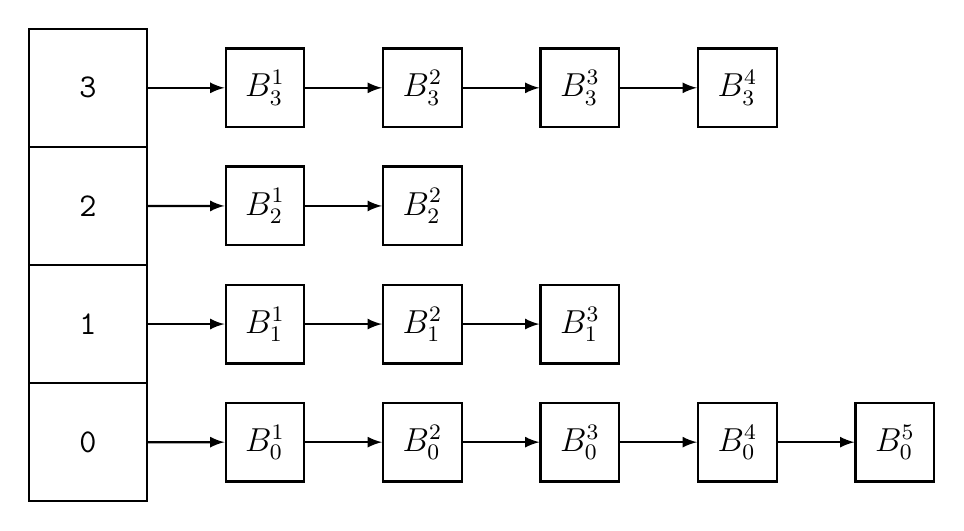
\begin{tikzpicture}[font={\fontsize{12pt}{12}\selectfont}]

    \node[rectangle, draw, color=black, thick, anchor=south west, minimum width=1.5cm, minimum height=1.5cm, inner sep=0pt] (c3) at (0, 4.5)    {\ttfamily 3};
    \node[rectangle, draw, color=black, thick, anchor=south west, minimum width=1.5cm, minimum height=1.5cm, inner sep=0pt] (c2) at (0, 3)      {\ttfamily 2};
    \node[rectangle, draw, color=black, thick, anchor=south west, minimum width=1.5cm, minimum height=1.5cm, inner sep=0pt] (c1) at (0, 1.5)    {\ttfamily 1};
    \node[rectangle, draw, color=black, thick, anchor=south west, minimum width=1.5cm, minimum height=1.5cm, inner sep=0pt] (c0) at (0, 0)      {\ttfamily 0};
   
    % C0 
    \node[rectangle, draw, color=black, thick, anchor=south west, minimum width=1cm, minimum height=1cm, inner sep=0pt] (b01) at (2.5, 0.25) {$B_0^1$};
    \node[rectangle, draw, color=black, thick, anchor=south west, minimum width=1cm, minimum height=1cm, inner sep=0pt] (b02) at (4.5, 0.25) {$B_0^2$};
    \node[rectangle, draw, color=black, thick, anchor=south west, minimum width=1cm, minimum height=1cm, inner sep=0pt] (b03) at (6.5, 0.25) {$B_0^3$};
    \node[rectangle, draw, color=black, thick, anchor=south west, minimum width=1cm, minimum height=1cm, inner sep=0pt] (b04) at (8.5, 0.25) {$B_0^4$};
    \node[rectangle, draw, color=black, thick, anchor=south west, minimum width=1cm, minimum height=1cm, inner sep=0pt] (b05) at (10.5, 0.25) {$B_0^5$};
    \draw[-latex, thick] (c0) -- (b01);
    \draw[-latex, thick] (b01) -- (b02);
    \draw[-latex, thick] (b02) -- (b03);
    \draw[-latex, thick] (b03) -- (b04);
    \draw[-latex, thick] (b04) -- (b05);

    % C1 
    \node[rectangle, draw, color=black, thick, anchor=south west, minimum width=1cm, minimum height=1cm, inner sep=0pt] (b11) at (2.5, 1.75) {$B_1^1$};
    \node[rectangle, draw, color=black, thick, anchor=south west, minimum width=1cm, minimum height=1cm, inner sep=0pt] (b12) at (4.5, 1.75) {$B_1^2$};
    \node[rectangle, draw, color=black, thick, anchor=south west, minimum width=1cm, minimum height=1cm, inner sep=0pt] (b13) at (6.5, 1.75) {$B_1^3$};
    \draw[-latex, thick] (c1) -- (b11);
    \draw[-latex, thick] (b11) -- (b12);
    \draw[-latex, thick] (b12) -- (b13);

    % C2 
    \node[rectangle, draw, color=black, thick, anchor=south west, minimum width=1cm, minimum height=1cm, inner sep=0pt] (b21) at (2.5, 3.25) {$B_2^1$};
    \node[rectangle, draw, color=black, thick, anchor=south west, minimum width=1cm, minimum height=1cm, inner sep=0pt] (b22) at (4.5, 3.25) {$B_2^2$};
    \draw[-latex, thick] (c2) -- (b21);
    \draw[-latex, thick] (b21) -- (b22);

    % C3 
    \node[rectangle, draw, color=black, thick, anchor=south west, minimum width=1cm, minimum height=1cm, inner sep=0pt] (b31) at (2.5, 4.75) {$B_3^1$};
    \node[rectangle, draw, color=black, thick, anchor=south west, minimum width=1cm, minimum height=1cm, inner sep=0pt] (b32) at (4.5, 4.75) {$B_3^2$};
    \node[rectangle, draw, color=black, thick, anchor=south west, minimum width=1cm, minimum height=1cm, inner sep=0pt] (b33) at (6.5, 4.75) {$B_3^3$};
    \node[rectangle, draw, color=black, thick, anchor=south west, minimum width=1cm, minimum height=1cm, inner sep=0pt] (b34) at (8.5, 4.75) {$B_3^4$};
    \draw[-latex, thick] (c3) -- (b31);
    \draw[-latex, thick] (b31) -- (b32);
    \draw[-latex, thick] (b32) -- (b33);
    \draw[-latex, thick] (b33) -- (b34);

    %\draw[latex-, thick] (c0.west) -- (-0.5, 0.75);

\end{tikzpicture}
}
                \caption{Exemple de liste de liste de zones mémoires associées à un PC}
                \label{fig_resumeFr_exBufferQueues}
            \end{figure}


    \item[Règle 4]
        La règle 4 impose que les accès à la DDR-SDRAM se fassent sans conflit au niveau des bancs. Ces accès étant rendus possibles aux partitions par l'utilisation de PCs, le calcul de l'ordonnancement du NoC doit s'effectuer avec une attention particulière portée aux PCs en provenance ou à destination des IONs. En calculant un ordonnancement tel que décrit en Section~\ref{ssec_resumeFr_reducInterference}, les problèmes de conflits d'accès à la DDR-SDRAM sont résolus par construction et ne nécessitent alors pas d'autre support en-ligne de la part de l'hyperviseur que celui de la gestion adéquate du NoC. En outre, en connaissant à l'avance les zones mémoires visées par les partitions (cf. règle 3) et en prenant pour hypothèse la configuration du contrôleur DDR-SDRAM décrite en Section~\ref{sssec_resumeFr_hypoHV}, le calcul de bornes sûres sur les temps nécessaires à la réalisation des transactions mémoire est largement simplifié par rapport au cas général, permettant ainsi d'effectuer efficacement la vérification hors-ligne du non dépassement des créneaux de communication des PCs.
\end{description}

\subsection{Validation expérimentale}
Afin de démontrer la capacité de notre modèle d'exécution à apporter une propriété d'isolation temporelle entre partitions concurrentes et de montrer que l'implémentation de celui-ci sur le \mppalong est possible, nous avons effectué une validation expérimentale basée sur un cas d'étude académique.
\subsubsection{Mise en \oe{}uvre}
Pour montrer l'isolation temporelle entre partitions, nous utilisons le cas d'étude \rosace~\cite{Pagetti2014} comme application de référence aux côtés de laquelle s'exécutera dans une autre partition une application de traitement d'image générant des interférences. Par l'étude du comportement de \rosace dans plusieurs scénarios de concurrence, nous cherchons à montrer son insensibilité aux interférences générées par la deuxième application.

Le cas d'étude \rosace est, bien que de taille modeste, représentatif dans sa structure des applications avioniques réelles, et ce notamment par son exécution multi-périodique complexe. Comme cela est montré sur la Figure~\ref{fig_resumeFr_rosace}, \rosace est composé d'un \emph{contrôleur} longitudinal de vol et d'un \emph{environnement de simulation} qui représente le modèle physique d'un avion. L'ensemble comporte 11 blocs s'exécutant à 50Hz, 100Hz ou 200Hz. 


\begin{figure}
    \centering
    \scalebox{1.5}{\begin{picture}(230,130)
        \put(0,0){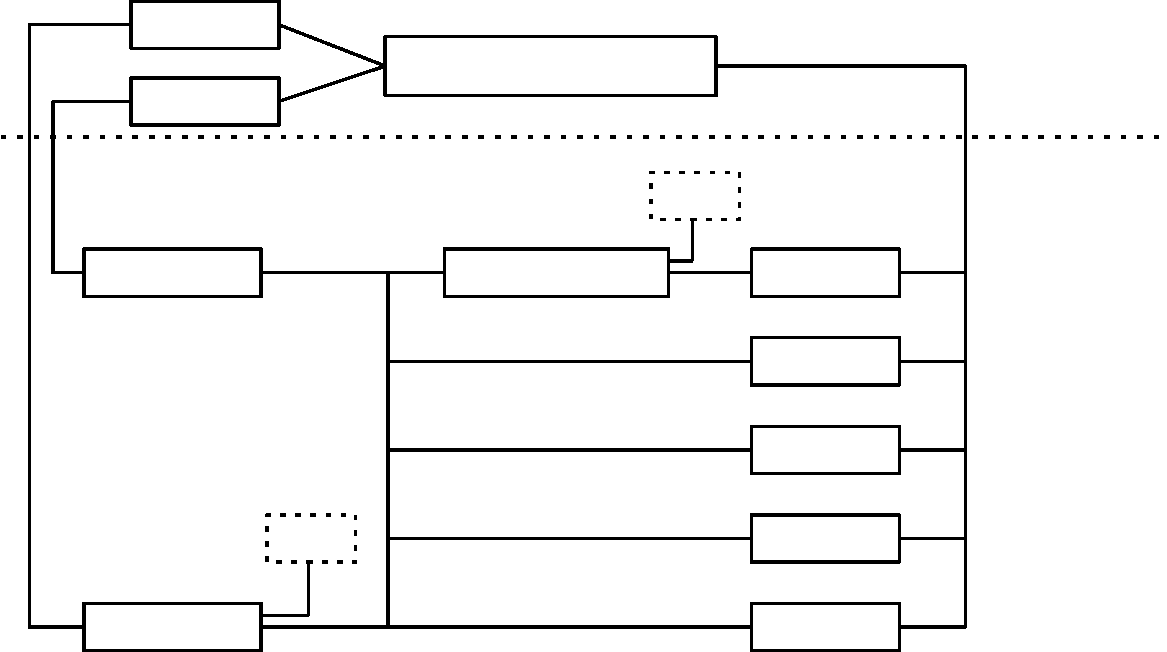
\includegraphics[width=230px]{imgs/pdf/implemExecModel_rosace.pdf}}
        % Blocs
        \put(32,123){\tiny engine}
        \put(30,107){\tiny elevator}
        \put(88,114){\tiny aircraft\_dynamics}
        \put(20,73){\tiny Vz\_control}
        \put(20,3){\tiny Va\_control}
        \put(155,73){\tiny h\_filter}
        \put(154,56){\tiny az\_filter}
        \put(152,38){\tiny Vz\_filter}
        \put(155,21){\tiny q\_filter}
        \put(153,3){\tiny Va\_filter}
        \put(94,73){\tiny altitude\_hold}
        \put(54,21){\tiny Va\_c}
        \put(132,89){\tiny h\_c}
        % Parts
        \put(195,115){\tiny Environnement de}
        \put(195,110){\tiny simulation}
        \put(195,92){\tiny Contrôleur}
        % Frequencies
        \put(59,28){\scalebox{0.9}{\tiny 10 Hz}}     % Va_c
        \put(135,96){\scalebox{0.9}{\tiny 10 Hz}}     % h_c
        \put(40,10){\scalebox{0.9}{\tiny 50 Hz}}     % Va_control
        \put(40,81){\scalebox{0.9}{\tiny 50 Hz}}     % Vz_control
        \put(120,81){\scalebox{0.9}{\tiny 50 Hz}}     % altitude_hold
        \put(164,81){\scalebox{0.9}{\tiny 100 Hz}}     % h_filter
        \put(164,63){\scalebox{0.9}{\tiny 100 Hz}}     % az_filter
        \put(164,46){\scalebox{0.9}{\tiny 100 Hz}}     % Vz_filter
        \put(164,28){\scalebox{0.9}{\tiny 100 Hz}}     % q_filter
        \put(164,10){\scalebox{0.9}{\tiny 100 Hz}}     % Va_filter
        \put(127,123){\scalebox{0.9}{\tiny 200 Hz}}     % ac_dyn
        \put(40,130){\scalebox{0.9}{\tiny 200 Hz}}     % engine
        \put(40,115){\scalebox{0.9}{\tiny 200 Hz}}     % elevator
        % Data
        \put(7,8){\scalebox{0.9}{\tiny $\delta_{\text{thc}}$}}
        \put(78,78){\scalebox{0.9}{\tiny Vz$_\text{c}$}}
        \put(11,83){\scalebox{0.9}{\tiny $\delta_\text{ec}$}}
        
        \put(141,79){\tiny h$_\text{f}$}
        \put(182,77){\tiny h}
        \put(140,61){\tiny az$_\text{f}$}
        \put(182,60){\tiny az}
        \put(139,43){\tiny Vz$_\text{f}$}
        \put(182,41){\tiny Vz}
        \put(141,26){\tiny q$_\text{f}$}
        \put(182,25){\tiny q}
        \put(140, 8){\tiny Va$_\text{f}$}
        \put(182, 7){\tiny Va}
        \put(61,123){\tiny T}
        \put(61,107){\tiny $\delta_\text{e}$}
    \end{picture}
}
    \caption{Contrôleur longitudinal de vol du cas d'étude \rosace}
    \label{fig_resumeFr_rosace}
\end{figure}

Nous avons fait le choix de placer l'ensemble de ces 11 blocs au sein d'un unique PN pour nos expériences en raison de la faible taille du code. Ce PN utilise 5 PEs sur lesquels l'exécution de \rosace est parallélisée et 3 bancs de SRAM locale. Pour rendre notre cas d'étude plus complet, nous avons ajouté à celui-ci un générateur de consignes appelé \emph{SPG}. Il est chargé de simuler les commandes du pilote en transmettant en-ligne des consignes d'altitude et de vitesse ($h_c$ et $V_{a_c}$) au contrôleur. Le SPG est placé dans un second PN connecté à \rosace par deux PCs pour transmettre les commandes et recevoir les sorties de simulation. Le SPG est également connecté à un ION par un troisième PC afin de loguer en DDR-SDRAM les traces de simulation. Ces 2 PNs et 3 PCs forment une partition dont la structure est présentée sur la Figure~\ref{fig_resumeFr_rosacePartBudget}

\begin{figure}
    \centering
    \scalebox{0.7}{
% X, Y, W, H, label, txt, moreparams
\newcommand\niceRect[7]{
    \node[rectangle, draw, color=black, thick, minimum width=#3cm, minimum height=#4cm, inner sep=0pt #7] (#5) at (#1,#2) {#6};
}

% X, Y, W, label, txt, moreparams
\newcommand\niceCirc[6]{
    \node[circle, draw, color=black, thick, minimum size=#3cm, inner sep=0pt #6] (#4) at (#1,#2) {#5};
}

\begin{tikzpicture}[font={\fontsize{12pt}{12}\selectfont}]
    \niceCirc{0}{1.5}{1}{c0}{C0}{}
    \niceRect{0}{0}{2}{1}{spg}{SPG}{}
    \draw[->, thick, dotted] (spg) -- (c0);
    
    \niceCirc{6}{1.5}{1}{c2}{C2}{}
    \niceRect{6}{0}{2}{1}{rosace}{\rosace}{}
    \draw[->, thick, dotted] (rosace) -- (c2);
    
    \niceCirc{0}{3.3}{1}{io1}{IO1}{}
    \niceRect{0}{4.8}{3}{1}{ddr}{\emph{DDR-SDRAM}}{}
    \draw[->, thick, dotted] (io1) -- (ddr);

    \draw[-latex, thick] (c0.30) -- node[above] {\footnotesize \PC{}$_1$ / 10Hz} (c2.150);
    \draw[-latex, thick] (c2.210) -- node[below] {\footnotesize \PC{}$_2$ / 200Hz} (c0.330);
    \draw[-latex, thick] (c0) -- (io1);
    \node[rotate=90] at (-0.9,2.4) {\footnotesize \PC{}$_3$ / 200Hz};

\end{tikzpicture}
}
    \caption{Budget de la partition de \rosace avec 2 \PN{}s et 3 \PC{}s}
    \label{fig_resumeFr_rosacePartBudget}
\end{figure}

L'application concurrente que nous considérons, appelée \emph{ImgInv}, effectue l'inversion d'une image en noir et blanc comme montré sur la Figure~\ref{fig_resumeFr_ImgInv_Lenna}. ImgInv est facilement parallélisable et est particulièrement configurable. L'ajustement de la taille des images à inverser permet de contrôler efficacement la charge de travail pour les PEs, l'empreinte mémoire de la partition et l'utilisation du NoC pour l'envoi et la réception d'images. Par ailleurs, l'implémentation d'ImgInv peut être qualifiée d'aisée.

\begin{figure}
    \centering
    \begin{subfigure}[b]{0.45\linewidth}
        \centering
        
\includegraphics[width=3cm]{imgs/png/implemExecModel_ImgInv_LennaNormal.png}
        \caption{Avant l'inversion}
        \label{fig_resumeFr_ImgInv_LennaNormal}
    \end{subfigure}
    \begin{subfigure}[b]{0.45\linewidth}
    \centering
        
\includegraphics[width=3cm]{imgs/png/implemExecModel_ImgInv_LennaInverted.png}
        \caption{Après l'inversion}
        \label{fig_resumeFr_ImgInv_LennaNormal}
    \end{subfigure}
    \caption{Exemple d'utilisation d'ImgInv}
    \label{fig_resumeFr_ImgInv_Lenna}
\end{figure}


\subsubsection{Scénarios}
A partir des deux applications décrites précédemment, nous avons exécuté 3 scénarios permettant de mettre en exergue la propriété d'isolation temporelle entre les deux partitions les hébergeant.
\begin{description}
    \item[Scénario 1, pas d'interférences]
        Dans un premier temps, nous avons exécuté la partition de \rosace seule sur le \mppalong afin de définir une exécution de référence qui sera par la suite comparée aux différents cas de concurrence. Comme montré sur la Figure~\ref{fig_resumeFr_rosacePartBudget}, le PN de \rosace est placé sur le cluster 2 et le PN du SPG est placé sur le cluster 0. Cette exécution nous a permis de valider fonctionnellement notre implémentation de \rosace en traitant à posteriori les données loguées en DDR-SDRAM. De plus, nous avons pu mesurer les temps d'exécution des 11 blocs comme montré sur la Figure~\ref{fig_resumeFr_ETrosace}. Sur cette figure les temps d'exécution minimaux et maximaux mesurés sont représentés par les lignes et les encadrés représentent la déviation standard centrée sur la moyenne. Chaque bloc est exécuté plus de 10~000 fois. Les temps d'exécution du bloc ``aircraft\_dynamics'' sont d'en moyenne 59~000 cycles d'horloge et ne sont pas représentés sur la figure pour plus de lisibilité.

\begin{figure}
    \centering
    \scalebox{1}{% GNUPLOT: LaTeX picture with Postscript
\begingroup
  \makeatletter
  \providecommand\color[2][]{%
    \GenericError{(gnuplot) \space\space\space\@spaces}{%
      Package color not loaded in conjunction with
      terminal option `colourtext'%
    }{See the gnuplot documentation for explanation.%
    }{Either use 'blacktext' in gnuplot or load the package
      color.sty in LaTeX.}%
    \renewcommand\color[2][]{}%
  }%
  \providecommand\includegraphics[2][]{%
    \GenericError{(gnuplot) \space\space\space\@spaces}{%
      Package graphicx or graphics not loaded%
    }{See the gnuplot documentation for explanation.%
    }{The gnuplot epslatex terminal needs graphicx.sty or graphics.sty.}%
    \renewcommand\includegraphics[2][]{}%
  }%
  \providecommand\rotatebox[2]{#2}%
  \@ifundefined{ifGPcolor}{%
    \newif\ifGPcolor
    \GPcolorfalse
  }{}%
  \@ifundefined{ifGPblacktext}{%
    \newif\ifGPblacktext
    \GPblacktexttrue
  }{}%
  % define a \g@addto@macro without @ in the name:
  \let\gplgaddtomacro\g@addto@macro
  % define empty templates for all commands taking text:
  \gdef\gplbacktext{}%
  \gdef\gplfronttext{}%
  \makeatother
  \ifGPblacktext
    % no textcolor at all
    \def\colorrgb#1{}%
    \def\colorgray#1{}%
  \else
    % gray or color?
    \ifGPcolor
      \def\colorrgb#1{\color[rgb]{#1}}%
      \def\colorgray#1{\color[gray]{#1}}%
      \expandafter\def\csname LTw\endcsname{\color{white}}%
      \expandafter\def\csname LTb\endcsname{\color{black}}%
      \expandafter\def\csname LTa\endcsname{\color{black}}%
      \expandafter\def\csname LT0\endcsname{\color[rgb]{1,0,0}}%
      \expandafter\def\csname LT1\endcsname{\color[rgb]{0,1,0}}%
      \expandafter\def\csname LT2\endcsname{\color[rgb]{0,0,1}}%
      \expandafter\def\csname LT3\endcsname{\color[rgb]{1,0,1}}%
      \expandafter\def\csname LT4\endcsname{\color[rgb]{0,1,1}}%
      \expandafter\def\csname LT5\endcsname{\color[rgb]{1,1,0}}%
      \expandafter\def\csname LT6\endcsname{\color[rgb]{0,0,0}}%
      \expandafter\def\csname LT7\endcsname{\color[rgb]{1,0.3,0}}%
      \expandafter\def\csname LT8\endcsname{\color[rgb]{0.5,0.5,0.5}}%
    \else
      % gray
      \def\colorrgb#1{\color{black}}%
      \def\colorgray#1{\color[gray]{#1}}%
      \expandafter\def\csname LTw\endcsname{\color{white}}%
      \expandafter\def\csname LTb\endcsname{\color{black}}%
      \expandafter\def\csname LTa\endcsname{\color{black}}%
      \expandafter\def\csname LT0\endcsname{\color{black}}%
      \expandafter\def\csname LT1\endcsname{\color{black}}%
      \expandafter\def\csname LT2\endcsname{\color{black}}%
      \expandafter\def\csname LT3\endcsname{\color{black}}%
      \expandafter\def\csname LT4\endcsname{\color{black}}%
      \expandafter\def\csname LT5\endcsname{\color{black}}%
      \expandafter\def\csname LT6\endcsname{\color{black}}%
      \expandafter\def\csname LT7\endcsname{\color{black}}%
      \expandafter\def\csname LT8\endcsname{\color{black}}%
    \fi
  \fi
  \setlength{\unitlength}{0.0500bp}%
  \begin{picture}(5616.00,4608.00)%
    \gplgaddtomacro\gplbacktext{%
      \csname LTb\endcsname%
      \put(726,1936){\makebox(0,0)[r]{\strut{} 300}}%
      \put(726,2203){\makebox(0,0)[r]{\strut{} 350}}%
      \put(726,2471){\makebox(0,0)[r]{\strut{} 400}}%
      \put(726,2738){\makebox(0,0)[r]{\strut{} 450}}%
      \put(726,3006){\makebox(0,0)[r]{\strut{} 500}}%
      \put(726,3273){\makebox(0,0)[r]{\strut{} 550}}%
      \put(726,3541){\makebox(0,0)[r]{\strut{} 600}}%
      \put(726,3808){\makebox(0,0)[r]{\strut{} 650}}%
      \put(726,4076){\makebox(0,0)[r]{\strut{} 700}}%
      \put(726,4343){\makebox(0,0)[r]{\strut{} 750}}%
      \put(1254,1804){\rotatebox{-270}{\makebox(0,0)[r]{\strut{}engine}}}%
      \put(1651,1804){\rotatebox{-270}{\makebox(0,0)[r]{\strut{}elevator}}}%
      \put(2047,1804){\rotatebox{-270}{\makebox(0,0)[r]{\strut{}Vz\_control}}}%
      \put(2444,1804){\rotatebox{-270}{\makebox(0,0)[r]{\strut{}Va\_control}}}%
      \put(2840,1804){\rotatebox{-270}{\makebox(0,0)[r]{\strut{}altitude\_hold}}}%
      \put(3237,1804){\rotatebox{-270}{\makebox(0,0)[r]{\strut{}h\_filter}}}%
      \put(3633,1804){\rotatebox{-270}{\makebox(0,0)[r]{\strut{}Vz\_filter}}}%
      \put(4030,1804){\rotatebox{-270}{\makebox(0,0)[r]{\strut{}q\_filter}}}%
      \put(4426,1804){\rotatebox{-270}{\makebox(0,0)[r]{\strut{}Va\_filter}}}%
      \put(4823,1804){\rotatebox{-270}{\makebox(0,0)[r]{\strut{}az\_filter}}}%
      \put(100,3139){\rotatebox{-270}{\makebox(0,0){\strut{}Cycles d'horloge}}}%
    }%
    \gplgaddtomacro\gplfronttext{%
    }%
    \gplbacktext
    \put(0,0){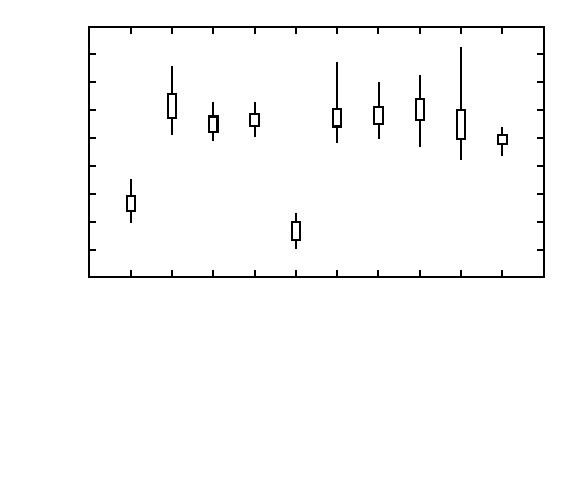
\includegraphics{imgs/pdf/implemExecModel_ETrosace.pdf}}%
    \gplfronttext
  \end{picture}%
\endgroup
}	
    \vspace{-5mm}
    \caption{Temps d'exécution des 11 blocs de \rosace}
	\label{fig_resumeFr_ETrosace}
\end{figure}

    \item[Scénario 2, interférences sur le NoC]
        Dans un second temps, nous avons ajouté au scénario 1 une partition contenant 2 instances d'ImgInv. Comme cela est montré sur la Figure~\ref{fig_resumeFr_scenario2budget}, chaque instance est placée dans un PN. Le premier est positionné sur le cluster 3 et le deuxième sur le cluster 4. Ces deux instances sont reliées par deux PCs dont les routes sont délibérément choisies pour partager des ressources NoC avec la partition de \rosace. Ainsi, la première instance d'ImgInv inverse une image et l'envoie par le NoC. A sa réception, la deuxième instance d'ImgInv inverse l'image et la renvoie à son tour et ainsi de suite. L'intérêt fonctionnel d'un tel travail est clairement faible mais cela permet de générer du trafic sur le NoC et ainsi de vérifier l'évitement des conflits avec \rosace. 

        \begin{figure}
    \centering
    \scalebox{0.7}{
% X, Y, W, H, label, txt, moreparams
\newcommand\niceRect[7]{
    \node[rectangle, draw, color=black, thick, minimum width=#3cm, minimum height=#4cm, inner sep=0pt #7] (#5) at (#1,#2) {#6};
}

% X, Y, W, label, txt, moreparams
\newcommand\niceCirc[6]{
    \node[circle, draw, color=black, thick, minimum size=#3cm, inner sep=0pt #6] (#4) at (#1,#2) {#5};
}

\begin{tikzpicture}[font={\fontsize{12pt}{12}\selectfont}]
    \niceCirc{0}{1.5}{1}{c0}{C0}{}
    \niceRect{0}{0}{2}{1}{spg}{SPG}{}
    \draw[->, thick, dotted] (spg) -- (c0);
    
    \niceCirc{4}{1.5}{1}{c2}{C2}{}
    \niceRect{4}{0}{2}{1}{rosace}{\rosace}{}
    \draw[->, thick, dotted] (rosace) -- (c2);
    
    \niceCirc{0}{3.3}{1}{io1}{IO1}{}
    \niceRect{0}{4.8}{3}{1}{ddr}{\emph{DDR-SDRAM}}{}
    \draw[->, thick, dotted] (io1) -- (ddr);

    \draw[-latex, thick] (c0.50) -- node[above] {\footnotesize \PC{}$_1$ / 10Hz} (c2.130);
    \draw[-latex, thick] (c2.230) -- node[below] {\footnotesize \PC{}$_2$ / 200Hz} (c0.310);
    \draw[-latex, thick] (c0) -- (io1);
    \node[rotate=90] at (-0.9,3.1) {\footnotesize \PC{}$_3$ / 200Hz};
    
    \niceCirc{-4}{1.5}{1}{c3}{C3}{}
    \niceRect{-4}{0}{2}{1}{imginv1}{\emph{ImgInv 1}}{}
    \draw[->, thick, dotted] (imginv1) -- (c3);
    \niceCirc{8}{1.5}{1}{c4}{C4}{}
    \niceRect{8}{0}{2}{1}{imginv2}{\emph{ImgInv 2}}{}
    \draw[->, thick, dotted] (imginv2) -- (c4);
    \draw[-latex, thick, dashed] (c3.30) -- node[very near end, above]  {\footnotesize \PC{}$_4$ / 500Hz} (c4.150);
    \draw[-latex, thick, dashed] (c4.210) -- node[very near end, below] {\footnotesize \PC{}$_5$ / 500Hz} (c3.330);

\end{tikzpicture}
}
    \caption{Configuration du deuxième scénario avec deux instances d'ImgInv partageant des ressources NoC avec \rosace}
    \label{fig_resumeFr_scenario2budget}
\end{figure}

Dans cette configuration, nous avons pu observer que les temps d'exécution des blocs de \rosace semblent insensibles à la nouvelle source d'interférences. Plus précisément, les meilleurs et pires temps d'exécution des 11 blocs mesurés lors du scénario 1 sont strictement égaux à ceux mesurés lors du scénario 2. De plus, en modifiant temporairement l'hyperviseur pour loguer les dates de réception des paquets reçus depuis le NoC, nous avons pu vérifier que 100\% de ceux-ci le sont lors des créneaux d'activation des PCs par lesquels ils sont envoyés. Cela implique qu'aucun paquet n'a subi de retard lié aux communications de la partition concurrente et que l'évitement des conflits sur le NoC semble respecté.





    \item[Scénario 3, interférences sur la DDR-SDRAM]
        Dans un dernier temps, nous avons ajouté au scénario 1 une partition contenant 1 instance d'ImgInv. Cette instance est placée dans un PN communiquant avec un ION afin de lire et d'écrire les images depuis/vers la DDR-SDRAM. Comme montré sur la Figure~\ref{fig_resumeFr_scenario3budget}, le PN d'ImgInv est placé sur le cluster 4 et l'ION est placé sur le même cluster IO que celui de \rosace. De plus, la zone mémoire depuis laquelle les images sont lues et écrites est placée dans le même banc mémoire que celui utilisé par \rosace pour simuler un cas d'interférence.
\begin{figure}
    \centering
    \scalebox{0.7}{
% X, Y, W, H, label, txt, moreparams
\newcommand\niceRect[7]{
    \node[rectangle, draw, color=black, thick, minimum width=#3cm, minimum height=#4cm, inner sep=0pt #7] (#5) at (#1,#2) {#6};
}

% X, Y, W, label, txt, moreparams
\newcommand\niceCirc[6]{
    \node[circle, draw, color=black, thick, minimum size=#3cm, inner sep=0pt #6] (#4) at (#1,#2) {#5};
}

\begin{tikzpicture}[font={\fontsize{12pt}{12}\selectfont}]
    \niceCirc{0}{1.5}{1}{c0}{C0}{}
    \niceRect{0}{0}{2}{1}{spg}{SPG}{}
    \draw[->, thick, dotted] (spg) -- (c0);
    
    \niceCirc{4}{1.5}{1}{c2}{C2}{}
    \niceRect{4}{0}{2}{1}{rosace}{\rosace}{}
    \draw[->, thick, dotted] (rosace) -- (c2);
    
    \niceCirc{0}{3.3}{1}{io1}{IO1}{}
    \niceRect{0}{4.8}{3}{1}{ddr}{\emph{DDR-SDRAM}}{}
    \draw[->, thick, dotted] (io1) -- (ddr);

    \draw[-latex, thick] (c0.50) -- node[above] {\footnotesize \PC{}$_1$ / 10Hz} (c2.130);
    \draw[-latex, thick] (c2.230) -- node[below] {\footnotesize \PC{}$_2$ / 200Hz} (c0.310);
    \draw[-latex, thick] (c0) -- (io1);
    \node[rotate=90] at (-0.9,2.4) {\footnotesize \PC{}$_3$ / 200Hz};
    
    \niceCirc{8}{3.3}{1}{io2}{IO2}{}
    \draw[->, thick, dotted] (io2) |- (ddr);

    \niceCirc{8}{1.5}{1}{c4}{C4}{}
    \niceRect{8}{0}{2}{1}{imginv2}{\emph{ImgInv}}{}
    \draw[->, thick, dotted] (imginv2) -- (c4);


    \draw[-latex, thick] (c4.40) -- (io2.320);
    \node[rotate=270] at (8.8,2.4) {\footnotesize \PC{}$_4$ / 500Hz};
    \node[rotate=90] at (7.2,2.4) {\footnotesize \PC{}$_5$ / 500Hz};
    \draw[-latex, thick] (io2.220) -- (c4.140);

\end{tikzpicture}
}
    \caption{Configuration du scénario avec une instance d'ImgInv partageant un banc de DDR-SDRAM avec \rosace}
    \label{fig_resumeFr_scenario3budget}
\end{figure}

        Dans cette configuration nous avons pu une nouvelle fois observer l'insensibilité des temps d'exécution des 11 blocs de \rosace aux interférences. Comme pour le scénario 2, les pires et meilleurs temps d'exécution de ces blocs sont strictement égaux à ceux mesurés lors du scénario 1. Une nouvelle fois, 100\% des paquets émis sur le NoC sont reçus pendant leur créneau d'envoi. Et enfin, en utilisant un \emph{interposeur} DDR-SDRAM pour récupérer de manière non intrusive les traces d'accès à la mémoire externe, nous avons pu observer que les transactions issues des deux partitions ne s'entrelacent pas et s'exécutent lors de périodes bien distinctes.

\end{description}

Avec ces trois scénarios, nous observons que, pour notre cas d'étude, la propriété d'isolation temporelle attendue semble être effective sur le système réel. Bien que n'apportant pas une preuve formelle de correction, ces résultats sont prometteurs et représentent déjà en eux-mêmes un intérêt certain d'un point de vue industriel.

\subsection{Synthèse}
Dans cette section, nous avons décrit l'implémentation de notre modèle d'exécution sur le \mppalong. Le respect de ses règles est assuré en-ligne par l'usage d'un hyperviseur en charge des différentes configurations matérielles et par des travaux de vérification budgétaire effectués hors-ligne pour garantir que toutes les règles sont respectées, et en particulier l'ordonnancement global du NoC. Nous avons montré avec un cas d'étude académique que la propriété d'isolation temporelle semble se vérifier en pratique, et ce malgré le partage de ressources au niveau du NoC ou de la DDR-SDRAM.

Au cours de cette section, nous avons pris l'hypothèse que les placements et ordonnancements des applications au sein de leurs budgets respectifs étaient connus. Dans le cas d'applications de grandes tailles, un calcul manuel est souvent rédhibitoire. Pour cette raison, nous montrons dans la section suivante comment, en utilisant la programmation par contraintes, il est possible de calculer \emph{automatiquement} et efficacement des placements et ordonnancements d'applications industrielles sur plusieurs clusters du \mppalong. 


\section{Validation des budgets}
\label{sec_resumeFr_validation}
Dans cette section, nous détaillons comment l'étape de \emph{Validation} de l'atelier d'intégration (Figure~\ref{fig_resumeFr_workFlow}) peut être automatisée en utilisation la programmation par contraintes. L'objectif de cette étape est de déterminer si une application peut s'exécuter correctement à l'intérieur du budget de sa partition. Pour répondre à cette problématique, nous proposons une approche permettant de calculer un placement et un ordonnancement d'une application sur un budget donné tout en respectant ses contraintes fonctionnelles et non fonctionnelles. D'une façon générale, nous considérons les budgets tels que formalisés en Section~\ref{ssec_resumeFr_paramEntreeWorkflow} et le modèle d'applications de la Section~\ref{ssec_resumeFr_appModel}.


\subsection{Choix des budgets}
A cette étape du processus d'intégration, les budgets sont connus. Le choix d'un budget plutôt qu'un autre peut avoir des conséquences majeures sur l'implémentation et sur les performances d'une application. Nous clarifions ici les hypothèses que nous prenons sur ces budgets et nous proposons des recommandations pour les déterminer en maximisant leurs chances d'être valides.
\subsubsection{Hypothèses}
\begin{description}
    \item[Chargement du code]
        Nous supposons dans cette section que les applications ne chargent \emph{pas} de code depuis la DDR-SDRAM externe. Cela implique que la totalité de l'application doit être stockée dans les mémoires SRAM locale des clusters de calcul. Cette hypothèse, bien que clairement contraignante, est motivée par deux raisons:
        \begin{enumerate}
            \item La problématique du chargement de code dans les clusters de calcul depuis la DDR-SDRAM est un sujet déjà abordé dans la littérature. Becker \etal~\cite{Becker16} ont par exemple proposé une méthode d'ordonnancement de \emph{Runnables} AUTOSAR sur un cluster du \mppalong en prenant en compte le chargement de leur code par le NoC. Avec notre approche, nous proposons une contribution qui est complémentaire aux travaux déjà effectués et faisant avancer l'état de l'art.
            \item Cette hypothèse implique que les applications de grande taille, c'est-à-dire trop grosses pour être stockées dans un seul cluster, soient réparties sur plusieurs. Ainsi, le problème de la gestion du NoC devient prépondérant dans notre cas. Nous voulons par ce travail adresser une problématique purement liée à l'architecture d'un processeur pluri-c\oe{}ur. Même s'il n'est pas évident que cette approche permette d'exploiter au maximum la capacité de calcul du \mppalong, elle reste particulièrement intéressante à étudier pour déterminer les solutions permettant la parallélisation massive sur une architecture basée NoC et qui deviendra inévitablement nécessaire à l'avenir compte tenu de la croissance des besoins en puissance de calcul.
        \end{enumerate}
    \item[Hyperviseur]
        Comme expliqué lors de la section précédente, notre capacité d'implémentation de l'hyperviseur pose quelques contraintes sur les budgets qui peuvent être choisis par les partitions. Tout d'abord, un banc de SRAM locale est réservé au sein de chaque cluster de calcul pour stocker le code de l'hyperviseur, les micro-codes DMA ainsi que les tables d'ordonnancement. Le nombre maximum de bancs de SRAM qu'un PN peut intégrer est donc borné par $N_b(pn) = 15$. De plus, les transferts DMA démarrant à l'activation de l'hyperviseur, les durées, périodes et offsets des PCs doivent être des multiples de la période d'activation de celui-ci. Avec une période d'activation de l'hyperviseur de $5 \mu s$ par exemple, un PC de période $20 \mu s$ sera défini par $T(pc) = 4$.
\end{description}

\subsubsection{Contraintes minimales}
A cette étape du processus d'intégration, les budgets doivent être connus. Il apparaît toutefois que les définir est souvent une tâche ardue qui peut parfois être contre-intuitive. Pour aider les développeurs d'application à définir la quantité de ressources dont ils ont besoin, nous donnons ici des recommandations sur le choix de ces budgets. Plus précisément, nous exprimons un jeu de conditions nécessaires (mais non suffisantes) qui, lorsque elles sont toutes satisfaites, n'apportent pas une garantie certaine de la validité d'un budget mais qui permettent de gagner en confiance sur la probabilité qu'il le sera.
\begin{description}
    \item[Contraintes mémoire]
        Les applications ne chargeant pas de code en-ligne depuis la DDR-SDRAM, elles doivent être intégralement stockées dans la SRAM locale des clusters de calcul. A partir de l'empreinte mémoire d'une application, nous pouvons tout d'abord vérifier que les PNs qui lui sont associés comprennent suffisamment de stockage pour la contenir complètement. Pour cela, la condition~\ref{eq_resumeFr_minCondMem} doit être remplie.
\begin{equation}
    \underset{pn \; \in \; \mathcal{N}_i}{\sum} N_b(pn) \times S_{bank}^{SRAM} \geq
    \underset{\tau_i^j \; \in \; S}{\sum} M_i^j
    \label{eq_resumeFr_minCondMem}
\end{equation}

    Par ailleurs, sachant que seules 15 bancs de SRAM peuvent être associés à chaque PN, il est impératif que le nombre de PNs compris dans une partition satisfasse la condition~\ref{eq_resumeFr_minCondMaxMem}.
\begin{equation}
    | \mathcal{N}_i | \geq 
    \left\lceil \dfrac{  \underset{\tau_i^j \; \in \; S}{\sum} M_i^j }{15 \times  S_{bank}^{SRAM}} \right\rceil
    \label{eq_resumeFr_minCondMaxMem}
\end{equation}


    \item[Contraintes computationelles]
        Comme pour la mémoire, il est possible de déterminer à partir du profil d'application des contraintes sur la capacité de calcul comprise dans un budget. Tout d'abord, nous pouvons définir le ratio d'utilisation d'une application $U$ par:

\begin{displaymath}
    U = \underset{\tau_i^j \; \in \; S}{\sum} \dfrac{C_i^j}{T_i}
\end{displaymath}

        Sachant que le nombre de PEs sur lesquels s'exécute l'application doit impérativement être plus grand que $U$, la condition~\ref{eq_resumeFr_minCondPEs} doit être remplie.
\begin{equation}
    \underset{pn \; \in \; \mathcal{N}_i}{\sum} N_c(pn) \geq \left\lceil U \right\rceil
    \label{eq_resumeFr_minCondPEs}
\end{equation}

        Par ailleurs, avec 16 PEs par cluster sur le \mppalong, le nombre de PNs d'un budget doit satisfaire la condition~\ref{eq_resumeFr_minCondMaxPEs}.
\begin{equation}
    | \mathcal{N}_i | \geq \left\lceil \dfrac{U}{16} \right\rceil
    \label{eq_resumeFr_minCondMaxPEs}
\end{equation}

\end{description}

\subsection{Processus de validation}
Notre méthode de validation repose sur l'utilisation de la programmation par contraintes. Cette approche permet de prendre en compte les modèles complexes de l'architecture du \mppalong et des applications tout en restant dans un cadre formel.

\subsubsection{Environnement de modélisation}
Plusieurs travaux explorent déjà la problématique du placement et de l'ordonnancement de tâches dépendantes sur des processeurs multi- ou pluri-c\oe{}urs en utilisant la programmation linéaire en nombres entiers (ou \emph{ILP} en anglais). De manière générale, ces approches souffrent de difficultés pour traiter des applications de grandes tailles. Ces difficultés sont souvent surmontées en utilisant des heuristiques de placement qui facilitent grandement le passage à l'échelle en abandonnant l'optimalité. Ici, nous utilisons un environnement de modélisation fondé sur la programmation par contraintes et qui a montré son efficacité pratique pour surmonter les difficultés de passage à l'échelle que nous avions également avec une formulation préliminaire basée ILP. Cet environnement est fondé sur la notion de \emph{Variable d'intervalle optionnelle}~\cite{Laborie08, Laborie09} introduite dans IBM ILOG CP Optimizer~\cite{OPL} depuis sa version 2.0. Une \emph{variable d'intervalle}, ici appelée $i$, représente une activité de durée finie. L'objectif du solveur est de calculer la date de début de $i$ notée $s(i)$. La durée de $i$ est notée $l(i)$. Chaque variable d'intervalle est définie dans une fenêtre temporelle $[ a(i) , d(i) ]$ où $a(i)$ et $d(i)$ représentent respectivement la date d'activation et l'échéance de $i$. Plus précisément, cela veut dire que tout ordonnancement calculé par le solveur doit vérifier $s(i) \geq a(i)$ et $s(i)+l(i) \leq d(i)$. 

\begin{figure}
    \centering
    \scalebox{0.8}{\begin{tikzpicture}
        \draw[thick, dashed] (3,-3) -- (3, 4);
        \draw[thick, dashed] (6,-3) -- (6, 4);
        \draw[thick, -latex] (0,0) -- (10,0);
        \draw  (3,0) node[draw, thick, fill=lightgray, rectangle, anchor=south west, inner sep=0pt, minimum width=3cm, minimum height=1cm] {\textbf{$i_1$}};
        \draw[thick, latex-latex] (3,1.5) -- (6,1.5) node[midway, above] {$l(i_1)$};
        \draw[thick] (3,0.1) -- (3,-0.1) node[below, fill=white] {$s(i_1) = ?$};
        \draw[thick] (1,0.1) -- (1,-0.1) node[below] {$a(i_1)$};
        \draw[thick] (9,0.1) -- (9,-0.1) node[below] {$d(i_1)$};

        \draw (-1.5, 0.5) node {$p(i_1) = 1$};
        \draw (-1.5, 3) node {$p(i_2) = 0$};
        \draw (-1.5, -2) node {$p(i_3) = 0$};
        \draw[thick, -latex] (0,2.5) -- (10,2.5);
        \draw  (3,2.5) node[draw, thick, fill=white, pattern=north west lines, rectangle, anchor=south west, inner sep=0pt, minimum width=3cm, minimum height=1cm] {$i_2$};
        \draw[thick, -latex] (0,-2.5) -- (10,-2.5);
        \draw  (3,-2.5) node[draw, thick, fill=white, pattern=north west lines, rectangle, anchor=south west, inner sep=0pt, minimum width=3cm, minimum height=1cm] {$i_3$};
    \end{tikzpicture}
}
    \caption{Exemple de 3 variables d'intervalle optionnelles $i_1$, $i_2$ et $i_3$ où seulement une est présente}
    \label{fig_resumeFr_condTimeInterval}
\end{figure}

Une variable d'intervalle est \emph{optionnelle} si sa présence dans la solution n'est systématiquement requise. Une variable d'intervalle optionnelle possède un attribut booléen $p(i)$ qui indique sa présence ou son absence dans la solution. Une variable absente ne sera alors pas prise en compte dans le jeu de contraintes à satisfaire. Cette notion peut notamment être mise à profit dans le cas où le problème à résoudre comporte non seulement une dimension temporelle (le calcul d'un ordonnancement) mais également une dimension spatiale (le placement d'intervalles sur des ressources). Par exemple, dans le cas où un jeu de tâches devrait être ordonnancé et placé sur un processeur multi-c\oe{}ur, une formulation naturelle comporterait pour chaque tâche un ensemble de variables d'intervalles optionnelles ($n$ intervalles pour $n$ c\oe{}urs) avec la contrainte qu'une et une seule de ces variables soit présente dans la solution finale. Cela encoderait alors l'allocation d'une tâche à un c\oe{}ur.



\begin{figure}
    \centering
    \begin{subfigure}[b]{\linewidth}
        \centering
        \scalebox{0.9}{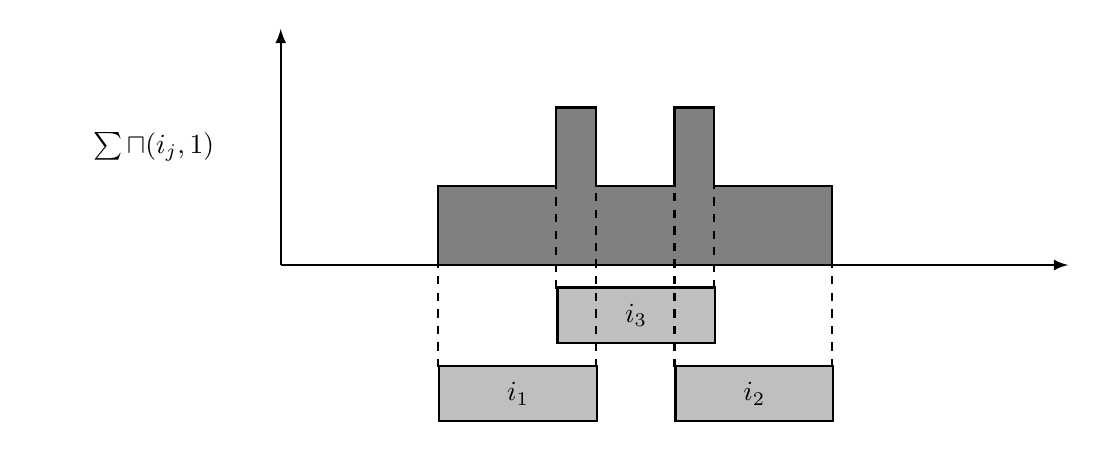
\begin{tikzpicture}
        \draw  (2,1) node[draw, thick, fill=lightgray, rectangle, anchor=south west, inner sep=0pt, minimum width=2cm, minimum height=0.7cm] {\textbf{$i_1$}};
        \draw  (5,1) node[draw, thick, fill=lightgray, rectangle, anchor=south west, inner sep=0pt, minimum width=2cm, minimum height=0.7cm] {\textbf{$i_2$}};
        \draw  (3.5,2) node[draw, thick, fill=lightgray, rectangle, anchor=south west, inner sep=0pt, minimum width=2cm, minimum height=0.7cm] {\textbf{$i_3$}};
        \draw[thick, -latex] (0,3) -- (0,6) node[midway, left, minimum width=3.2cm] {$\sum \sqcap(i_j, 1)$};

        \draw[thick, fill=gray] (2,3) -- (2,4) -- (3.5,4) -- (3.5,5) -- (4,5) -- (4,4) -- (5,4) -- (5,5) -- (5.5,5) -- (5.5,4) -- (7,4) -- (7,3);
        \draw[thick, dashed] (2,1.7) -- (2,3);
        \draw[thick, dashed] (3.5,2.7) -- (3.5,4);
        \draw[thick, dashed] (4,1.7) -- (4,4);
        \draw[thick, dashed] (5,1.7) -- (5,4);
        \draw[thick, dashed] (5.5,2.7) -- (5.5,4);
        \draw[thick, dashed] (7,1.7) -- (7,3);
        \draw[thick, -latex] (0,3) -- (10,3);
    \end{tikzpicture}
}
        \caption{Une fonction porte appliquée à $i_1$, $i_2$ et $i_3$ \emph{sans} contrainte}
        \label{fig_resumeFr_pulseFunctionNoConst}
    \end{subfigure}\vspace{5mm}
    \begin{subfigure}[b]{\linewidth}
        \centering
        \scalebox{0.9}{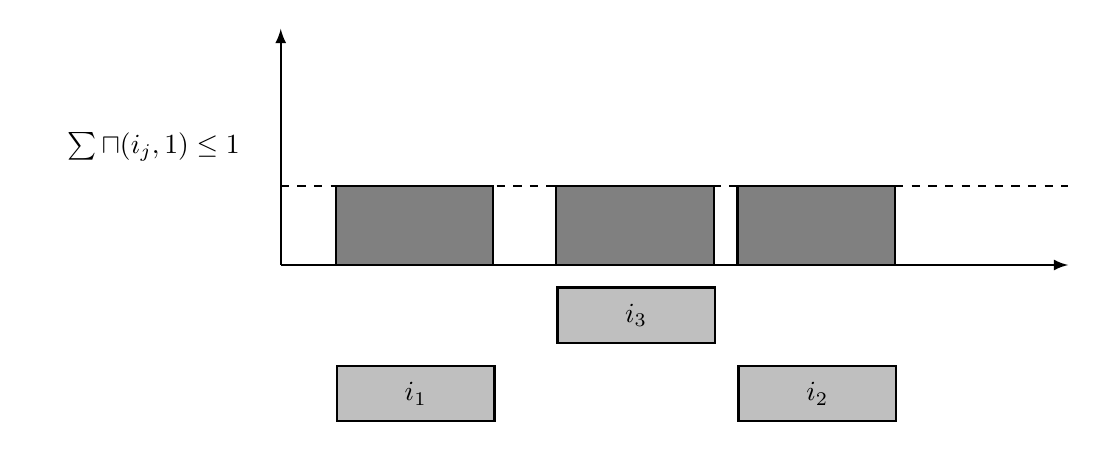
\begin{tikzpicture}
        \draw  (0.7,1) node[draw, thick, fill=lightgray, rectangle, anchor=south west, inner sep=0pt, minimum width=2cm, minimum height=0.7cm] {\textbf{$i_1$}};
        \draw  (5.8,1) node[draw, thick, fill=lightgray, rectangle, anchor=south west, inner sep=0pt, minimum width=2cm, minimum height=0.7cm] {\textbf{$i_2$}};
        \draw  (3.5,2) node[draw, thick, fill=lightgray, rectangle, anchor=south west, inner sep=0pt, minimum width=2cm, minimum height=0.7cm] {\textbf{$i_3$}};
        \draw[thick, -latex] (0,3) -- (0,6) node[midway, left, minimum width=3.2cm] {$\sum \sqcap(i_j, 1) \leq 1$};

        \draw[thick, fill=gray] (0.7,3) -- (0.7,4) -- (2.7,4) -- (2.7,3) -- (3.5,3) -- (3.5,4) -- (5.5,4) -- (5.5,3) -- (5.8,3) -- (5.8,4) -- (7.8,4) -- (7.8,3);
        \draw[thick, dashed] (0,4) -- (10,4);
        \draw[thick, -latex] (0,3) -- (10,3);
    \end{tikzpicture}
}
        \caption{Une fonction porte appliquée à $i_1$, $i_2$ et $i_3$ \emph{avec} contraintes}
        \label{fig_resumeFr_pulseFunctionWithConst}
    \end{subfigure}
    \caption{Exemple d'utilisation des fonctions portes sur 3 intervalles $i_1$, $i_2$ et $i_3$}
    \label{fig_resumeFr_pulseFunction}
\end{figure}

IBM ILOG CP Optimizer permet également l'utilisation du concept de \emph{fonction cumulative}. Elle représente l'usage cumulatif qui est fait d'une ressource par des activités au cours du temps. On les utilise généralement afin de restreindre l'utilisation d'une ressource à des capacités limitées. Dans notre formulation, nous n'utiliserons que les fonctions \emph{portes} notées $\sqcap(i, h)$ avec $i$ une variable d'intervalle et $h$ la quantité de ressource consommée sur la durée de $i$. La Figure~\ref{fig_resumeFr_pulseFunction} représente un exemple d'utilisation d'une telle fonction porte avec notamment un cas contraint mettant en \oe{}uvre l'exclusion mutuelle des 3 intervalles considérés. 

Afin de simplifier les notations, nous utiliserons la notation suivante pour forcer la présence d'une seule variable d'intervalle optionnelle parmi un ensemble $I = \{ i_1 , \ldots , i_n \}$:
        \begin{displaymath}
            \oplus(I)=1 \Leftrightarrow \underset{i \in I}{\sum} p(i) = 1
        \end{displaymath}

Du plus nous définissons comme suit l'opérateur de précédence entre deux intervalles:
        \begin{displaymath}
            i_1 \to i_2 \Leftrightarrow s(i_1) + l(i_1) \leq s(i_2)
        \end{displaymath}


\subsubsection{Formulation du problème}
Notre objectif est de calculer un placement et un ordonnancement d'une application $\mathcal{A} = <\tau , \delta>$ sur un budget $<\mathcal{N} , \mathcal{I} , \mathcal{C} , \mathcal{B} >$. L'utilisation de la notion de variable d'intervalle implique de travailler au niveau des instances et pas des tâches elles mêmes. Sur une hyper-période $$T_H = \underset{\tau_i \in \tau}{\text{lcm}} (T_i)$$
avec $T_i$ la période de $\tau_i$, chaque tâche peut être activée plusieurs fois. Nous parlerons du k-ième \emph{job} de $\tau_i$, noté $\tau_{i,k}$, pour se référer à sa k-ième activation. De même, la k-ième activation de la sous-tâche $\tau_i^j$ sera appelée k-ième sous-job, noté $\tau_{i,k}^j$. L'ensemble de tous les sous-jobs exécutés sur une hyper-période est noté $S$. Les relations de précédences entre sous-tâches d'une même tâche sont dupliquées entre sous-jobs du même job. La k-ième production d'une donnée $\delta_x$ par le sous-job $\tau_{i,k}^j$ est notée $\delta_{x,k}$.

La gestion des buffers d'entrée et de sortie de l'application se traduit par des envois ou des réceptions de données vers ou depuis la DDR-SDRAM externe. Ainsi, la gestion de ces données n'est pas différente de celle des données entre sous-tâches à l'exception du fait que les PCs utilisés pour les envoyer sont ceux connectés aux IONs.

Pour notre problème de placement et d'ordonnancement, nous considérons deux types de variables de décision.

\begin{description}
    \item[Les sous-jobs sur les PNs]
        Nous associons à chaque sous-job $\tau_{i,k}^j$ un ensemble de $|\mathcal{N}|$ variables d'intervalles conditionnelles. On note $j( \tau_{i,k}^j , pn )$ la variable représentant l'allocation de $\tau_{i,k}^j$ sur le PN $pn$. La durée de chacun de ces intervalles est égale au WCET de la sous-tâche correspondante, soit plus formellement $l( j( \tau_{i,k}^j , pn ) ) = C_i^j$. La fenêtre d'existence de chaque intervalle correspond à la fenêtre d'existence du sous-job associé sur l'hyper-période, c'est-à-dire $[ k \times T_i , (k+1) \times T_i ]$. Cela est représenté sur la Figure~\ref{fig_resumeFr_decVarJobs}
        \begin{figure}
            \centering
            \scalebox{0.9}{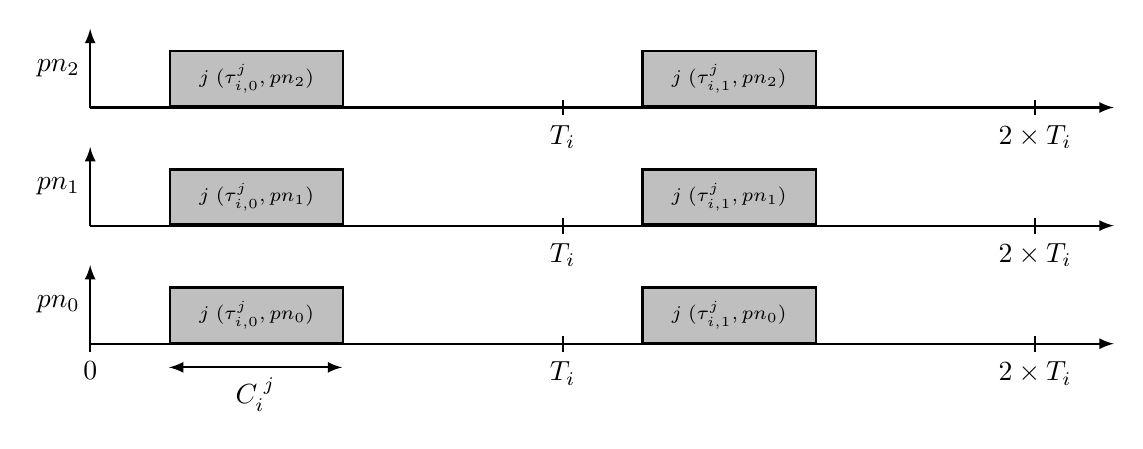
\begin{tikzpicture}
\draw[thick, -latex] (0,0) -- (13,0);
\draw[thick, -latex] (0,1.5) -- (13,1.5);
\draw[thick, -latex] (0,3) -- (13,3);
\draw[thick, -latex] (0,0) -- (0,1) node[midway, left] {$pn_0$};
\draw[thick, -latex] (0,1.5) -- (0,2.5) node[midway, left] {$pn_1$};
\draw[thick, -latex] (0,3) -- (0,4) node[midway, left] {$pn_2$};


\draw  (1,3) node[draw, thick, fill=lightgray, rectangle, anchor=south west, inner sep=0pt, minimum width=2.2cm, minimum height=0.7cm]      {\scriptsize $ j \; ( \tau_{i,0}^j, pn_2 )$};
\draw  (1, 1.5) node[draw, thick, fill=lightgray, rectangle, anchor=south west, inner sep=0pt, minimum width=2.2cm, minimum height=0.7cm]   {\scriptsize $ j \; ( \tau_{i,0}^j, pn_1 )$};
\draw  (1,0) node[draw, thick, fill=lightgray, rectangle, anchor=south west, inner sep=0pt, minimum width=2.2cm, minimum height=0.7cm]      {\scriptsize $ j \; ( \tau_{i,0}^j, pn_0 )$};
\draw[thick, latex-latex] (1,-0.3) -- (3.2,-0.3) node[midway, below] {$C_i^{\; j}$};

\draw[thick] (0,0.1) -- (0, -0.1) node [below] {$0$};
\draw[thick] (6,0.1) -- (6, -0.1) node [below] {$T_i$};
\draw[thick] (6,1.6) -- (6, 1.4) node [below] {$T_i$};
\draw[thick] (6,3.1) -- (6, 2.9) node [below] {$T_i$};


\draw[thick] (12,1.6) -- (12, 1.4) node [below] {$2 \times T_i$};
\draw[thick] (12,0.1) -- (12, -0.1) node [below] {$2 \times T_i$};
\draw[thick] (12,3.1) -- (12, 2.9) node [below] {$2 \times T_i$};

\draw  (7,0) node[draw, thick, fill=lightgray, rectangle, anchor=south west, inner sep=0pt, minimum width=2.2cm, minimum height=0.7cm]      {\scriptsize $ j \; ( \tau_{i,1}^j, pn_0 )$};
\draw  (7, 1.5) node[draw, thick, fill=lightgray, rectangle, anchor=south west, inner sep=0pt, minimum width=2.2cm, minimum height=0.7cm]   {\scriptsize $ j \; ( \tau_{i,1}^j, pn_1 )$};
\draw  (7,3) node[draw, thick, fill=lightgray, rectangle, anchor=south west, inner sep=0pt, minimum width=2.2cm, minimum height=0.7cm]      {\scriptsize $ j \; ( \tau_{i,1}^j, pn_2 )$};
\end{tikzpicture}
}
            \caption{6 intervalles représentant 1 sous-tâche $\tau_i^j$ avec 2 sous-jobs ordonnançable sur 3 PNs}
            \label{fig_resumeFr_decVarJobs}
        \end{figure}


    \item[Les données sur les PCs]
        Nous associons à chaque instance de donnée $\delta_{x,k}$ un ensemble de $|\mathcal{C}|$ variables d'intervalles conditionnelles. On note $d( \delta_{x,k}, pc )$ l'intervalle représentant l'envoi de $\delta_{x,k}$ au travers du PC $pc$. Lorsque $d( \delta_{x,k}, pc )$ est présente dans la solution finale, cela implique que  $\delta_{x,k}$ est envoyée depuis le PN $src(pc)$ à destination du PN $dst(pc)$ au travers de $pc$. Dans le cas des données, la durée des intervalles les représentant n'est pas liée au temps nécessaire à l'envoi de la donnée sur le NoC. La durée de ces intervalles est fixée comme égale à la largeur d'un créneau d'accès au NoC sur le PC considéré. Plus formellement, on définit $l( d( \delta_{x,k}, pc ) ) = C(pc)$. La limite sur la quantité de données qui peuvent être envoyées via un PC sera assurée par la suite en utilisant des fonctions cumulatives. La date de début d'une variable d'intervalle $d( \delta_{x,k}, pc )$ encode ici l'allocation de cette donnée à un slot spécifique de son $pc$. La fenêtre d'existence des intervalles de données est égale à celle de leur sous-job producteur.
\end{description}



\subsubsection{Contraintes}
Notre formulation du problème d'allocation et d'ordonnancement comporte plusieurs familles de contraintes avec des objectifs bien précis. Nous détaillons ces contraintes ici.
\begin{description}
    \item[Placement des sous-jobs]
        Chaque sous-job ne peut être exécuté que par un seul PN. Ceci se traduit par la contrainte~\ref{eq_resumeFr_oneSubjobPerPN} qui impose qu'une seule variable d'intervalle soit présente pour chaque sous-job.
\begin{equation}
    \label{eq_resumeFr_oneSubjobPerPN}
    \forall \tau_{i,k}^j \in S ,  
    \oplus(\{ j( \tau_{i,k}^j , pn ) \; | \; \forall pn \in \mathcal{N}\})=1
\end{equation}

        Si les sous-jobs d'une même sous-tâche pouvaient s'exécuter sur différents PNs, c'est-à-dire migrer d'un PN à un autre entre deux activations, cela impliquerait que le code de cette sous-tâche soit dupliqué sur plusieurs PNs et mettrait ainsi de la pression sur une ressource sensible: la SRAM locale. De plus, les données statiques de la sous-tâche devraient être envoyées d'un cluster à l'autre pour garantir une exécution cohérente, et impliqueraient alors davantage de trafic sur une deuxième ressource sensible: le NoC. Pour éviter ces problèmes et simplifier notre formulation, nous interdisons ces migrations en forçant tous les sous-jobs d'une même sous-tâche à s'exécuter sur le même PN. Cela est traduit par la contrainte~\ref{eq_resumeFr_allSubjobsSamePN}.
\begin{equation}
    \label{eq_resumeFr_allSubjobsSamePN}
    \forall \tau_{i,k}^j \in S, \; \forall pn \in \mathcal{N}, \;
    p( j( \tau_{i,k}^j, pn )) = p( j( \tau_{i,(k+1) \% \frac{T_H}{T_i}}^j, pn ))
\end{equation}

    \item[Utilisation des PNs]
        Le nombre de PEs au sein d'un PN étant limité, le nombre de sous-jobs qui peuvent s'exécuter en parallèle sur ce PN doit l'être également. C'est ce qu'exprime la contrainte~\ref{eq_resumeFr_constPNcoreUtil} en utilisant des fonctions cumulatives.i
\begin{equation}
    \label{eq_resumeFr_constPNcoreUtil}
    \forall pn \in \mathcal{N} , \;
    \underset{\forall \tau_{i,k}^j \in S}{\sum} \sqcap( j( \tau_{i,k}^j , pn ),1) \leq N_c(pn)
\end{equation}

        Par ailleurs, les sous-tâches allouées à un PN doivent être stockables sur celui-ci en intégralité. La contrainte~\ref{eq_resumeFr_constPNmemUtil} garantit le respect de cette limitation mémoire. Il peut être remarqué que la contrainte~\ref{eq_resumeFr_constPNmemUtil} ne vise que la première activation de chaque sous-tâche (avec $\tau_{i,0}^j $). En effet, les migrations étant interdites, toutes les activations de la même sous-tâche utiliseront le même code.

\begin{equation}
    \label{eq_resumeFr_constPNmemUtil}
    \forall pn \in \mathcal{N} , \;
    \underset{ \tau_i^j \in S }{\sum} p( j( \tau_{i,0}^j , pn ) ) \times M_i^j \leq N_b(pn) \times S_{bank}^{SRAM}
\end{equation}


    \item[Placement des données]
        Le placement d'une donnée sur un PC dépend du positionnement de sa sous-tâche productrice et de celui de ses sous-tâches consommatrices. Lorsque producteur et consommateur sont sur le même PN, la communication s'effectue par mémoire partagée au sein du cluster et aucun envoi de donnée sur le NoC n'est nécessaire. Dès qu'un consommateur est positionné sur un PN distant, la donnée produite doit être émise sur le PC adéquat. Ceci est capturé par la contrainte~\ref{eq_resumeFr_constDataPCmapping}.

\begin{equation}
    \label{eq_resumeFr_constDataPCmapping}
    \begin{array}{l}
        \forall pc \in \mathcal{C}, \; \forall \delta_{x} \in \delta,  \\
        \hspace{5mm} \Big( \; p(j(prod(\delta_{x,0}), src(pc))) \; \land \underset{\tau_{i,0}^j \in cons(\delta_{x,0})}{\sum} p(j(\tau_{i,0}^j , dst(pc))) \geq 1   \Big)  = p( \delta_{x,0} , pc  ) 
    \end{array}
\end{equation}
        
        Les sous-tâches ne pouvant migrer, les données à envoyer doivent toujours l'être sur les mêmes PCs. Ceci se traduit par la contrainte~\ref{eq_resumeFr_constDataJobSamePC}.
\begin{equation}
    \label{eq_resumeFr_constDataJobSamePC}
    \forall pc \in \mathcal{C}, \; \forall \delta_{x,k} \in \delta, \; 
    p( d( \delta_{x,k} , pc ) ) = p( d( \delta_{x,k+1} , pc ) )
\end{equation}
        
        Enfin, la date de début des intervalles de données encode l'allocation d'une donnée à un certain slot de son PC. Pour cela, sa date début doit être alignée avec le début d'un slot du PC en question, comme cela est fait via la contrainte~\ref{eq_resumeFr_constStartDateData}.
\begin{equation}
    \label{eq_resumeFr_constStartDateData}
    \forall pc \in \mathcal{C}, \; \forall \delta_{x,k} \in \delta, \; 
    s( d( \delta_{x,k}, pc ) ) \; \% \; T(pc) = O(pc)
\end{equation}


    \item[Utilisation des PCs]


        La quantité de données qui peut être envoyée au travers des PCs doit être limitée pour correspondre aux capacités des liens NoC et des DMAs. Notre modèle d'exécution garantissant l'absence de conflits sur le NoC, nous pouvons déduire le nombre de flits qui peuvent traverser un PC $pc$ durant sa durée d'activation comme
\begin{displaymath}
    N_{flit}^{PC} (pc) = C(pc) - (R(pc) + 1) \times \Delta_L - R(pc)\times \Delta_S 
\end{displaymath}
avec $\Delta_L$ la latence d'un lien NoC et $\Delta_S$ la latence d'un switch en absence de collision. En notant $N_{flit}^{total}(m_x)$ le nombre de flits nécessaires à l'envoi des $m_x$ octets d'une donnée $\delta_x$, on peut contraindre la quantité de données à envoyer à travers chaque activation d'un PC via la contrainte~\ref{eq_resumeFr_consPcUtilData}. Cela est représenté graphiquement sur la Figure~\ref{fig_resumeFr_consPcUtilData}.
\begin{equation}
    \label{eq_resumeFr_consPcUtilData}
    \forall pc \in \mathcal{C} , 
    \sum_{\delta_{x,k} \in \delta} \sqcap \Big( d(\delta_{x,k} , pc) , N_{flit}^{total}(m_x) + N_{flit}^{gap} \Big) \leq N_{flit}^{PC} (pc)
\end{equation}

\begin{figure}
    \centering
    \scalebox{0.9}{   
\newcommand\ttask[7]{\draw  ( #1 , #2 ) node[draw, thick, fill= #3 , rectangle, anchor=south west, inner sep=0pt, minimum width=#4cm, minimum height= #5cm #7] { #6 };}

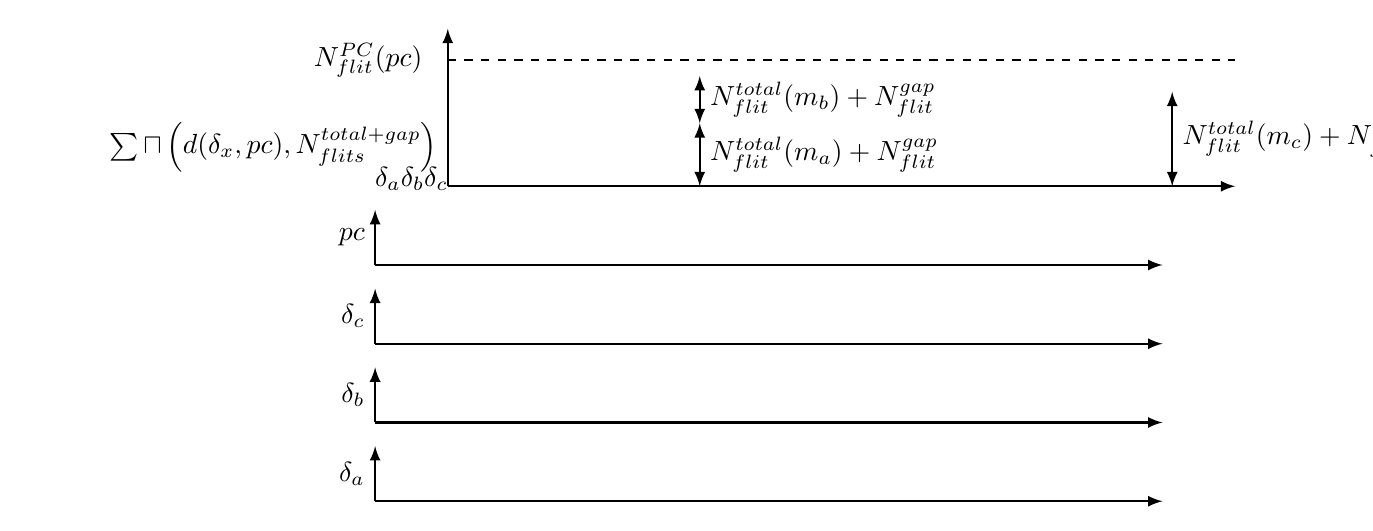
\begin{tikzpicture}
    \draw (12,0) node { };
    \draw[thick, -latex] (0,-1) -- (10,-1);
    \draw[thick, -latex] (0,-1) -- (0,-0.3) node[left, midway] {$pc$};
    \ttask{1}{-1}{gray}{2}{0.5}{}{}
    \ttask{7}{-1}{gray}{2}{0.5}{}{}
    
    \ttask{1}{-2}{}{2}{0.5}{}{, pattern=north west lines}
    \ttask{1}{-3}{}{2}{0.5}{}{, pattern=north west lines}
    \ttask{1}{-4}{}{2}{0.5}{}{, pattern=north west lines}
    \ttask{7}{-2}{}{2}{0.5}{}{, pattern=north west lines}
    \ttask{7}{-3}{}{2}{0.5}{}{, pattern=north west lines}
    \ttask{7}{-4}{}{2}{0.5}{}{, pattern=north west lines}
    
    \draw[thick, -latex] (0,-2) -- (10,-2);
    \draw[thick, -latex] (0,-2) -- (0,-1.3) node[left, midway] {$\delta_c$};
    \draw[thick, -latex] (0,-3) -- (10,-3);
    \draw[thick, -latex] (0,-3) -- (0,-2.3) node[left, midway] {$\delta_b$};
    \draw[thick, -latex] (0,-4) -- (10,-4);
    \draw[thick, -latex] (0,-4) -- (0,-3.3) node[left, midway] {$\delta_a$};
    \ttask{1}{-3}{lightgray}{2}{0.5}{}{}
    \ttask{1}{-4}{lightgray}{2}{0.5}{}{}
    \ttask{7}{-2}{lightgray}{2}{0.5}{}{}
    
    \ttask{1}{0}{lightgray}{2}{0.8}{$\delta_a$}{}
    \ttask{1}{0.8}{lightgray}{2}{0.6}{$\delta_b$}{}
    \ttask{7}{0}{lightgray}{2}{1.2}{$\delta_c$}{} 
    \draw[thick, -latex] (0,0) -- (10,0);
    %\draw[thick, -latex, align=left] (0,0) -- (0,2) node[left, near start] {$\sum \sqcap \left( d(\delta_x,pc) ,\right.$ \\ $ \left. N_{flit}^{total}(m_x) + N_{flit}^{gap}  \right)$};
    \draw[thick, -latex, align=left] (0,0) -- (0,2) node[left, near start] {$\sum \sqcap \left( d(\delta_x,pc) , N_{flits}^{total+gap}  \right)$};
    
    \draw[thick, latex-latex] (3.2, 0) -- (3.2, 0.8) node[midway, right] {$N_{flit}^{total} ( m_a ) + N_{flit}^{gap}$};
    \draw[thick, latex-latex] (3.2, 0.8) -- (3.2, 1.4) node[midway, right] {$N_{flit}^{total} ( m_b ) + N_{flit}^{gap}$};
    \draw[thick, latex-latex] (9.2, 0) -- (9.2, 1.2) node[midway, right] {$N_{flit}^{total} ( m_c ) + N_{flit}^{gap}$};
    
    \draw[thick, dashed] (0, 1.6) -- (10, 1.6);
    \draw (-0.2, 1.6) node[anchor=east] {$N_{flit}^{PC}(pc)$};
\end{tikzpicture}
}
    \caption{Limitation de la quantité de données qui peut être envoyée durant l'activation d'un PC en utilisant les fonctions cumulatives sur les variables d'intervalle des données}
    \label{fig_resumeFr_consPcUtilData}
\end{figure}

        Le terme $N_{flit}^{gap}$ de la contrainte~\ref{eq_resumeFr_consPcUtilData} représente le nombre de flits perdus lors d'un saut du DMA d'une zone mémoire à une autre. En le comptant pour toutes données envoyées, on fait l'hypothèse conservative que les données sont placées dans des zones mémoire non contigües et que le DMA doit sauter de l'une à l'autre lors d'un envoi. Si l'on intégrait au problème d'ordonnancement le calcul des positions de données en mémoire, il serait possible de concaténer des données et d'éviter le surcoût systématique de $N_{flit}^{gap}$. S'il est clair que cela pourrait permettre de gagner en performance, il est moins évident que l'accroissement de la complexité soit assez faible pour pouvoir traiter des problèmes de grandes tailles avec les machines et les solveurs actuels. L'évaluation de ce compromis apparaît toutefois comme une perspective intéressante d'amélioration de notre travail.

        Les DMA n'étant capables de traiter automatiquement qu'une quantité limitée de travaux, le nombre de zones non contigües qui peuvent être émises pendant une seule activation doit être contraint. Avec $N_{bufs}^{DMA}$ le nombre maximum de zones mémoire que le DMA peut traiter de manière autonome, cela est traduit dans la contrainte~\ref{eq_resumeFr_consPcUtilDDMA}.

\begin{equation}
    \label{eq_resumeFr_consPcUtilDDMA}
    \forall pc \in \mathcal{C} , 
    \sum_{\delta_{x,k} \in \delta} \sqcap ( d(\delta_{x,k} , pc) , 1 ) \leq N_{bufs}^{DMA}
\end{equation}

    \item[Relations de précédence]
        Dans notre modèle d'application, les contraintes de précédences ne sont imposées qu'entre deux sous-tâches échangeant des données. Ces données peuvent être classifiées en deux catégories:
        \begin{itemize}
            \item les données \emph{en avant} sont produites par la sous-tâche parente de la relation de précédence. Plus formellement, avec une précédence $(\tau_i^j , \tau_i^l )$ où $\tau_i^j$ doit s'exécuter avant $\tau_i^l$ ($\tau_i^j$ est donc la sous-tâche parente), $\delta_x$ est une donnée en avant si $(\tau_i^j = prod(\delta_x)) \land (\tau_i^l \in cons(\delta_x))$;
            \item les données \emph{en arrière} sont produites par la sous-tâche fille de la relation de précédence. C'est-à-dire que la donnée produite sera consommée lors de la prochaine activation de la sous-tâche parente. Plus formellement, avec une précédence $(\tau_i^j , \tau_i^l )$ où $\tau_i^j$ est parente, $\delta_x$ est une donnée en arrière si $(\tau_i^j \in cons(\delta_x)) \land (\tau_i^l = prod(\delta_x))$.
        \end{itemize}
        
        Lorsque les deux sous-tâches contraintes par une relation de précédence sont placées sur le même PN, la communication est assurée par mémoire partagée et il suffit de garantir l'ordre d'exécution de ces sous-tâches avec la contrainte~\ref{eq_resumeFr_constPrecFwSamePN}.
\begin{equation}
    \label{eq_resumeFr_constPrecFwSamePN}
    \forall (\tau_{i,k}^j , \tau_{i,k}^l) \in P_{i,k}, \; \forall pn \in \mathcal{N} , \; 
    j( \tau_{i,k}^j , pn ) \to j( \tau_{i,k}^l , pn )
\end{equation}

        Si les deux sous-tâches sont sur des PNs différents, la donnée doit être émise au travers du NoC. Avec des données en avant, nous utilisons l'intervalle de la donnée en question comme pivot de précédence pour garantir la précédence entre les sous-tâches. C'est-à-dire que le sous-job producteur de la donnée est forcé de s'exécuter avant le début du créneau d'envoi de la donnée sur son PC comme cela est fait avec la contrainte~\ref{eq_resumeFr_constDataProdOrder}. Et ensuite, le sous-job consommateur est quant à lui contraint de démarrer après la fin du slot d'envoi pour garantir la bonne réception de cette donnée au moment de son exécution. Cela est traduit par la contrainte~\ref{eq_resumeFr_constDataFwConsumerPrec}. La Figure~\ref{fig_resumeFr_constFwDataPrec} montre une représentation graphique de cette notion de pivot.

\begin{equation}
    \label{eq_resumeFr_constDataProdOrder}
    \forall pc \in \mathcal{C} , \; \forall \delta_{x,k} \in \delta , \;
    j(prod(\delta_{x,k}) , src(pc)) \to d( \delta_{x,k} , pc )   
\end{equation}

\begin{equation}
    \label{eq_resumeFr_constDataFwConsumerPrec}
    \begin{array}{l}
        \forall (\tau_{i,k}^j , \tau_{i,k}^l) \in P_{i,k}, \; \forall pc \in \mathcal{C} , \; \forall \delta_{x,k} \in \delta , \;  \\
        \hspace{5mm} (\tau_{i,k}^j = prod(\delta_{x,k})) \land (\tau_{i,k}^l \in cons(\delta_{x,k})) 
        \Rightarrow d( \delta_{x,k} , pc ) \to j(\tau_{i,k}^l , dst(pc)) 
    \end{array}
\end{equation}

\begin{figure}
    \centering
    \scalebox{0.9}{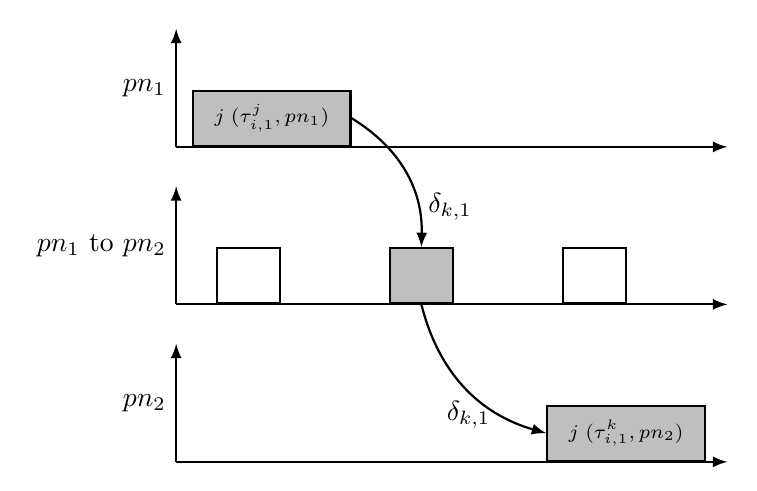
\begin{tikzpicture}
    \draw[thick, -latex] (0,0) -- (7,0); 
    \draw[thick, -latex] (0,2) -- (7,2); 
    \draw[thick, -latex] (0,4) -- (7,4); 
    \draw[thick, -latex] (0,0) -- (0,1.5) node[midway, left] {$pn_2$}; 
    \draw[thick, -latex] (0,2) -- (0,3.5) node[midway, left] {$pn_1$ to $pn_2$}; 
    \draw[thick, -latex] (0,4) -- (0,5.5) node[midway, left] {$pn_1$};

    \draw  (0.2,4) node[draw, thick, fill=lightgray, rectangle, anchor=south west, inner sep=0pt, minimum width=2cm, minimum height=0.7cm] (jpn1) { \scriptsize $ j \; ( \tau_{i,1}^j, pn_1 )$};
    \draw  (4.7,0) node[draw, thick, fill=lightgray, rectangle, anchor=south west, inner sep=0pt, minimum width=2cm, minimum height=0.7cm] (jpn2) { \scriptsize $ j \; ( \tau_{i,1}^k, pn_2 )$};

    \draw  (0.5,2) node[draw, thick, fill=white, rectangle, anchor=south west, inner sep=0pt, minimum width=0.8cm, minimum height=0.7cm] {};
    \draw  (2.7,2) node[draw, thick, fill=lightgray, rectangle, anchor=south west, inner sep=0pt, minimum width=0.8cm, minimum height=0.7cm] (dpc) {};
    \draw  (4.9,2) node[draw, thick, fill=white, rectangle, anchor=south west, inner sep=0pt, minimum width=0.8cm, minimum height=0.7cm] {};
    \draw (jpn1.east) edge[thick, -latex, bend left] node[near end, right] {$\delta_{k,1}$} (dpc.north);
    \draw (dpc.south) edge[thick, -latex, bend right] node[near end, left] {$\delta_{k,1}$} (jpn2.west);
\end{tikzpicture}
}
    \caption{Intervalle de donnée utilisé comme pivot pour mettre en \oe{}uvre une précédence entre deux sous-jobs placés sur 2 PNs distants.}
    \label{fig_resumeFr_constFwDataPrec}
\end{figure}

        Dans le cas des données en arrière, la donnée consommée par le sous-job parent $\tau_{i,k}^j$ de la précédence est celle produite par le sous-job précédent de sous-tâche fille $\tau_{i,k-1}^l$. Lorsque producteurs et consommateurs sont sur le même PN, la contrainte~\ref{eq_resumeFr_constPrecFwSamePN} suffit à assurer un comportement correct. En effet, la fenêtre d'exécution de la donnée produite par $\tau_{i,k-1}^l$ termine au début de celle de la fenêtre d'exécution $\tau_{i,k}^j$. En conséquence l'ordre d'émission de consommation est naturellement assuré par construction. Si les deux sous-tâches sont placées sur des PNs différents, il faut garantir que le sous-job parent se termine avant l'envoi de la donnée produite par le sous-job fils afin d'éviter la consommation d'une donnée ``trop fraîche''. Cela est fait avec la contrainte~\ref{eq_resumeFr_constBwDataPrec}.
\begin{equation}
    \label{eq_resumeFr_constBwDataPrec}
    \begin{array}{l}
        \forall (\tau_{i,k}^j , \tau_{i,k}^l) \in P_{i,k}, \; \forall pc \in \mathcal{C} , \; \forall \delta_{x,k} \in \delta , \;  \\
        \hspace{5mm} (\tau_{i,k}^j \in cons(\delta_{x,k})) \land (\tau_{i,k}^l = prod(\delta_{x,k}))
        \Rightarrow j(\tau_{i,k}^j , dst(pc)) \to d( \delta_{x,k} , pc )  
    \end{array}
\end{equation}

    \item[Déterminisme]
        Certaines données peuvent être échangées par des sous-tâches non contraintes par une relation de précédence. Dans le cas où un sous-job producteur et un sous-job consommateur s'exécuteraient en même temps, il n'est pas évident que l'ordre de production et de consommation de la donnée soit connu, et il est même possible qu'il varie d'une exécution à l'autre. Nous qualifions cette possible irrépétabilité d'exécution de l'ordonnancement comme non déterministe. Pour éliminer ce non déterminisme et rendre les exécutions répétables, nous forçons l'ordre de production et de consommation des données non contraintes, quel qu'il soit, à rester consistant d'une exécution à l'autre. Quand les sous-tâches productrices et consommatrices sont assignées au même PN, on interdit leur recouvrement temporel par le biais de la contrainte~\ref{eq_resumeFr_constDetermSamePNs}.
\begin{equation}
    \label{eq_resumeFr_constDetermSamePNs}
    \begin{array}{l}
        \forall \delta_{x,k} \in \delta , \; \forall \tau_{i,l}^j \in cons( \delta_{x,k} ), \; \forall pn \in \mathcal{N}, \\
        \hspace{5mm} ( prod(\delta_{x,k}), \tau_{i,l}^j ) \notin P_k \land (\tau_{i,l}^j, prod(\delta_{x,k})) \notin P_k \\
        \hspace{5mm} \Rightarrow \sqcap ( j(prod(\delta_{x,k}), pn) ,1) + \sqcap ( j(\tau_{i,l}^j, pn) ,1) \leq 1
    \end{array}
\end{equation}

Dans le cas où producteurs et consommateurs sont placés sur des PNs différents, c'est le créneau de réception de la donnée et l'exécution du sous-job consommateur qui ne doivent pas être simultanés. Ceci est traduit par la contrainte~\ref{eq_resumeFr_constDetermDiffPNs}.

\begin{equation}
    \label{eq_resumeFr_constDetermDiffPNs}
    \begin{array}{l}
        \forall \delta_{x,k} \in \delta ,\; \forall \tau_{i,l}^j \in cons( \delta_{x,k} ), \; \forall pc \in \mathcal{C}, \\
        \hspace{5mm} ( prod(\delta_{x,k}), \tau_{i,l}^j ) \notin P_k \land (\tau_{i,l}^j, prod(\delta_{x,k})) \notin P_k \\
        \hspace{5mm} \Rightarrow \sqcap ( d(\delta_{x,k}, pc) ,1) + \sqcap ( j(\tau_{i,l}^j, dst(pc)) ,1) \leq 1
    \end{array}
\end{equation}

        
\end{description}



\subsection{Résultats expérimentaux}
Afin d'évaluer la capacité de notre approche à traiter des problèmes de grande taille, nous avons effectué une série d'expérimentations basées sur une application industrielle d'Airbus. L'objectif de ces expériences est multiple. En effet, nous voulons non seulement être capables de calculer automatiquement l'ordonnancement et le placement de l'application dans son budget mais également étudier l'impact de ce budget sur les performances de notre ordonnanceur et évaluer jusqu'à quel niveau de charge applicative notre méthode est applicable. Ainsi, nous explorons les solutions existantes dans un espace de 3 paramètres:
\begin{description}
    \item[Charge applicative]
        Afin de simuler une augmentation de charge applicative, nous intégrons un paramètre permettant de raccourcir les périodes des tâches sans changer les durées d'exécution des sous-tâches. Ce faisant, le ratio d'utilisation $U$ augmente et la recherche d'un ordonnancement valide s'avère être de plus en plus difficile. Nous chercherons ici à déterminer jusqu'à quel niveau de charge applicative nous arrivons à trouver des ordonnancements corrects. Nous réduirons artificiellement les périodes en jouant sur un paramètre $k_{div}$ permettant de réduire la période des tâches avec $\widetilde{T}_i = \frac{256-k_{div}}{256} \times T_i$. Avec $k_{div} \in [ 0 , 255 ]$, les périodes des applications $\widetilde{T}_i \in [ T_i/256 , T_i ]$.
    \item[Réduction du budget]
        Afin de comprendre l'impact de la modification d'un budget sur la performance de notre ordonnanceur, nous expérimentons avec plusieurs configurations de budgets qui sont des variations autour d'un budget originel. Tout d'abord, nous considérons trois configurations différentes de PNs. Avec $n_{pn}^{orig}$ le nombre originel de PNs, nous étudierons des budgets avec des nombre de PNs variant suivant $ n_{pn}^{orig} \leq |\mathcal{N}| \leq n_{pn}^{orig} + 2$. Cela nous permettra d'identifier si l'augmentation de la puissance de calcul allouée à la partition (plus de PNs veut dire plus de PEs) permet de supporter une charge applicative supérieure. Nous évaluerons également l'impact des modifications sur les PCs en faisant varier leur durée. Avec $C_{orig}(pc)$ la durée originelle d'un PC, nous testerons trois configurations avec des durées comprises dans $[ C_{orig}(pc) , C_{orig}(pc) +2 ]$.
    \item[Configuration des DMAs]
        Enfin, nous évaluons notre cas d'étude avec plusieurs configurations possibles de DMAs. Pour cela, nous faisons varier le nombre de zones de mémoire non contigües $N_{bufs}^{DMA}$ qu'un DMA peut traiter de manière autonome (notamment utilisé dans contrainte~\ref{eq_resumeFr_consPcUtilDDMA}). Comme expliqué en Section~\ref{sssec_resumeFr_repectReglesEM}, le temps nécessaire pour la configuration du DMA par le RM dépend du nombre de zones à traiter. En réduisant celui-ci, nous réduisons l'autonomie du DMA mais réduisons également le WCET de l'hyperviseur qui peut ainsi être activé plus souvent. En augmentant $N_{bufs}^{DMA}$, le DMA sera plus autonome mais la période d'activation de l'hyperviseur devra être plus longue et permettra d'exprimer les durées et périodes des PCs à un grain moins fin. En évaluant plusieurs configurations de $N_{bufs}^{DMA}$ comprises dans $[4,32]$ nous cherchons à identifier le meilleur compromis pour le type d'application considérée.
\end{description}

\subsubsection{Description du cas d'étude}
Notre cas d'étude est basé sur une application réelle d'Airbus de grande taille. Elle suit le modèle défini en Section~\ref{ssec_resumeFr_appModel} et possède plusieurs tâches aux périodes harmoniques. Sur une hyper-période, on dénombre environ 100~000 sous-jobs et données produites. Lorsque l'on considère cette application sous la forme d'intervalles, on arrive à plusieurs millions de variables de décisions et de contraintes à satisfaire.

Nous faisons les choix pour les budgets et donc pour l'implémentation de cette application:
\begin{description}
    \item[1 PE par PN]
        Pour toutes les expérimentations menées sur notre cas d'étude, nous forçons systématiquement le nombre de PEs alloués à chaque PN à être $N_c(pn) = 1$. Cela permet d'une part d'éliminer les interférences entre PEs de la même partition au niveau de la SRAM et donc de réduire les WCETs et d'autre part d'accentuer la nécessité d'une gestion fine du NoC pour la distribution sur plusieurs clusters. Bien que notre formulation du problème permette une parallélisation dans et entre les clusters de calculs, nous concentrons notre étude sur la gestion du NoC qui est le vrai défi nouveau sur une architecture pluri-c\oe{}urs.
    \item[PCs courts et symétriques]
        Nous choisissons de relier l'ensemble des PNs de notre partition avec des PCs \emph{courts} et \emph{symétriques}. Court signifie que la durée $C(pc)$ est choisie la plus faible petite, c'est-à-dire, de l'ordre de grandeur de la période d'activation de l'hyperviseur. De ce fait, nous espérons réduire les délais NoC subis lors de précédences avec des données en avant qui représentent le véritable coût d'une exécution distribuée. Symétrique signifie que, pour des raisons de simplifications, tous les PCs ont des durées et des périodes égales. Seuls les offsets changent pour éviter les conflits.
\end{description}

\subsubsection{Analyse des résultats}



\pgfplotstableread{imgs/tex/dat/validation_expeSpeedups/6_1_8.dat}\kdivvsdurSixUnHuit
\pgfplotstableread{imgs/tex/dat/validation_expeSpeedups/6_1_16.dat}\kdivvsdurSixUnSeize
\pgfplotstableread{imgs/tex/dat/validation_expeSpeedups/6_1_24.dat}\kdivvsdurSixUnVingtquatre
\pgfplotstableread{imgs/tex/dat/validation_expeSpeedups/6_1_32.dat}\kdivvsdurSixUnTrentedeux
\pgfplotstableread{imgs/tex/dat/validation_expeSpeedups/6_2_8.dat}\kdivvsdurSixDeuxHuit
\pgfplotstableread{imgs/tex/dat/validation_expeSpeedups/6_2_16.dat}\kdivvsdurSixDeuxSeize
\pgfplotstableread{imgs/tex/dat/validation_expeSpeedups/6_2_24.dat}\kdivvsdurSixDeuxVingtquatre
\pgfplotstableread{imgs/tex/dat/validation_expeSpeedups/6_2_32.dat}\kdivvsdurSixDeuxTrentedeux
\pgfplotstableread{imgs/tex/dat/validation_expeSpeedups/6_3_8.dat}\kdivvsdurSixTroisHuit
\pgfplotstableread{imgs/tex/dat/validation_expeSpeedups/6_3_16.dat}\kdivvsdurSixTroisSeize
\pgfplotstableread{imgs/tex/dat/validation_expeSpeedups/6_3_24.dat}\kdivvsdurSixTroisVingtquatre
\pgfplotstableread{imgs/tex/dat/validation_expeSpeedups/6_3_32.dat}\kdivvsdurSixTroisTrentedeux
\pgfplotstableread{imgs/tex/dat/validation_expeSpeedups/7_1_8.dat}\kdivvsdurSeptUnHuit
\pgfplotstableread{imgs/tex/dat/validation_expeSpeedups/7_1_16.dat}\kdivvsdurSeptUnSeize
\pgfplotstableread{imgs/tex/dat/validation_expeSpeedups/7_1_24.dat}\kdivvsdurSeptUnVingtquatre
\pgfplotstableread{imgs/tex/dat/validation_expeSpeedups/7_1_32.dat}\kdivvsdurSeptUnTrentedeux
\pgfplotstableread{imgs/tex/dat/validation_expeSpeedups/7_2_8.dat}\kdivvsdurSeptDeuxHuit
\pgfplotstableread{imgs/tex/dat/validation_expeSpeedups/7_2_16.dat}\kdivvsdurSeptDeuxSeize
\pgfplotstableread{imgs/tex/dat/validation_expeSpeedups/7_2_24.dat}\kdivvsdurSeptDeuxVingtquatre
\pgfplotstableread{imgs/tex/dat/validation_expeSpeedups/7_2_32.dat}\kdivvsdurSeptDeuxTrentedeux
\pgfplotstableread{imgs/tex/dat/validation_expeSpeedups/7_3_8.dat}\kdivvsdurSeptTroisHuit
\pgfplotstableread{imgs/tex/dat/validation_expeSpeedups/7_3_16.dat}\kdivvsdurSeptTroisSeize
\pgfplotstableread{imgs/tex/dat/validation_expeSpeedups/7_3_24.dat}\kdivvsdurSeptTroisVingtquatre
\pgfplotstableread{imgs/tex/dat/validation_expeSpeedups/7_3_32.dat}\kdivvsdurSeptTroisTrentedeux
\pgfplotstableread{imgs/tex/dat/validation_expeSpeedups/8_1_8.dat}\kdivvsdurHuitUnHuit
\pgfplotstableread{imgs/tex/dat/validation_expeSpeedups/8_1_16.dat}\kdivvsdurHuitUnSeize
\pgfplotstableread{imgs/tex/dat/validation_expeSpeedups/8_1_24.dat}\kdivvsdurHuitUnVingtquatre
\pgfplotstableread{imgs/tex/dat/validation_expeSpeedups/8_1_32.dat}\kdivvsdurHuitUnTrentedeux
\pgfplotstableread{imgs/tex/dat/validation_expeSpeedups/8_2_8.dat}\kdivvsdurHuitDeuxHuit
\pgfplotstableread{imgs/tex/dat/validation_expeSpeedups/8_2_16.dat}\kdivvsdurHuitDeuxSeize
\pgfplotstableread{imgs/tex/dat/validation_expeSpeedups/8_2_24.dat}\kdivvsdurHuitDeuxVingtquatre
\pgfplotstableread{imgs/tex/dat/validation_expeSpeedups/8_2_32.dat}\kdivvsdurHuitDeuxTrentedeux
\pgfplotstableread{imgs/tex/dat/validation_expeSpeedups/8_3_8.dat}\kdivvsdurHuitTroisHuit
\pgfplotstableread{imgs/tex/dat/validation_expeSpeedups/8_3_16.dat}\kdivvsdurHuitTroisSeize
\pgfplotstableread{imgs/tex/dat/validation_expeSpeedups/8_3_24.dat}\kdivvsdurHuitTroisVingtquatre
\pgfplotstableread{imgs/tex/dat/validation_expeSpeedups/8_3_32.dat}\kdivvsdurHuitTroisTrentedeux
\begin{figure}
    \centering
    \begin{subfigure}[b]{0.3\textwidth} \begin{tikzpicture} \begin{axis}[xscale=0.65,yscale=0.36,xmin=3187500,xmax=48000000,ymin=0,ymax=12000,ytick={0,2000,4000,6000,8000,10000,10800,12000},yticklabels={,,,,,,,},scaled y ticks = false, scaled x ticks = false,, xticklabels=none, legend style={at={(1.5,2.7)},anchor=north east, font=\tiny}]
                \addplot[mark=none, red, dashed, samples=2, domain=3187500:48000000, forget plot] {10800};
                \addplot[mark=*, color=blue] table[x index=0, y index=1]          {\kdivvsdurSixUnHuit};
                \addplot[mark=square*, color=red] table[x index=0, y index=1]     {\kdivvsdurSixUnSeize};
                \addplot[mark=diamond*, color=brown] table[x index=0, y index=1]  {\kdivvsdurSixUnVingtquatre};
                \addplot[mark=triangle*, color=black] table[x index=0, y index=1] {\kdivvsdurSixUnTrentedeux};
                \legend{ $N_{bufs}^{DMA}=8$, $N_{bufs}^{DMA}=16$, $N_{bufs}^{DMA}=24$, $N_{bufs}^{DMA}=32$ }
    \end{axis} \end{tikzpicture} \caption{ $n_{pn}^{orig}$, $C_{orig}(pc)$ } \label{fig_validation_speedupDurationSmallestBudget}
    \end{subfigure}
    \begin{subfigure}[b]{0.3\textwidth} \begin{tikzpicture} \begin{axis}[xscale=0.65,yscale=0.36,xmin=3187500,xmax=48000000,ymin=0,ymax=12000,ytick={0,2000,4000,6000,8000,10000,10800,12000},yticklabels={,,,,,,,},scaled y ticks = false, scaled x ticks = false,, xticklabels=none]
                \addplot[mark=none, red, dashed, samples=2, domain=3187500:48000000, forget plot] {10800};
                \addplot[mark=*, color=blue] table[x index=0, y index=1]          {\kdivvsdurSixDeuxHuit};
                \addplot[mark=square*, color=red] table[x index=0, y index=1]     {\kdivvsdurSixDeuxSeize};
                \addplot[mark=diamond*, color=brown] table[x index=0, y index=1]  {\kdivvsdurSixDeuxVingtquatre};
                \addplot[mark=triangle*, color=black] table[x index=0, y index=1] {\kdivvsdurSixDeuxTrentedeux};
        \end{axis} \end{tikzpicture} \caption{ $n_{pn}^{orig}$, $C_{orig}(pc)+1$ }
    \end{subfigure}
    \begin{subfigure}[b]{0.3\textwidth} \begin{tikzpicture} \begin{axis}[xscale=0.65,yscale=0.36,xmin=3187500,xmax=48000000,ymin=0,ymax=12000,ytick={0,2000,4000,6000,8000,10000,10800,12000},yticklabels={,,,,,,,},scaled y ticks = false, scaled x ticks = false,, xticklabels=none]
                \addplot[mark=none, red, dashed, samples=2, domain=3187500:48000000, forget plot] {10800};
                \addplot[mark=*, color=blue] table[x index=0, y index=1]          {\kdivvsdurSixTroisHuit};
                \addplot[mark=square*, color=red] table[x index=0, y index=1]     {\kdivvsdurSixTroisSeize};
                \addplot[mark=diamond*, color=brown] table[x index=0, y index=1]  {\kdivvsdurSixTroisVingtquatre};
                \addplot[mark=triangle*, color=black] table[x index=0, y index=1] {\kdivvsdurSixTroisTrentedeux};
        \end{axis} \end{tikzpicture} \caption{ $n_{pn}^{orig}$, $C_{orig}(pc)=2$ }
    \end{subfigure}

    \begin{subfigure}[b]{0.3\textwidth} \begin{tikzpicture} \begin{axis}[xscale=0.65,yscale=0.36,xmin=3187500,xmax=48000000,ymin=0,ymax=12000,ytick={0,2000,4000,6000,8000,10000,10800,12000},yticklabels={,,,,,,,},scaled y ticks = false, scaled x ticks = false,, xticklabels=none]
                \addplot[mark=none, red, dashed, samples=2, domain=3187500:48000000, forget plot] {10800};
                \addplot[mark=*, color=blue] table[x index=0, y index=1]          {\kdivvsdurSeptUnHuit};
                \addplot[mark=square*, color=red] table[x index=0, y index=1]     {\kdivvsdurSeptUnSeize};
                \addplot[mark=diamond*, color=brown] table[x index=0, y index=1]  {\kdivvsdurSeptUnVingtquatre};
                \addplot[mark=triangle*, color=black] table[x index=0, y index=1] {\kdivvsdurSeptUnTrentedeux};
        \end{axis} \end{tikzpicture} \caption{ $n_{pn}^{orig}+1$, $C_{orig}(pc)$ } \label{fig_validation_speedupDurationBudget_d}
    \end{subfigure}
    \begin{subfigure}[b]{0.3\textwidth} \begin{tikzpicture} \begin{axis}[xscale=0.65,yscale=0.36,xmin=3187500,xmax=48000000,ymin=0,ymax=12000,ytick={0,2000,4000,6000,8000,10000,10800,12000},yticklabels={,,,,,,,},scaled y ticks = false, scaled x ticks = false,, xticklabels=none]
                \addplot[mark=none, red, dashed, samples=2, domain=3187500:48000000, forget plot] {10800};
                \addplot[mark=*, color=blue] table[x index=0, y index=1]          {\kdivvsdurSeptDeuxHuit};
                \addplot[mark=square*, color=red] table[x index=0, y index=1]     {\kdivvsdurSeptDeuxSeize};
                \addplot[mark=diamond*, color=brown] table[x index=0, y index=1]  {\kdivvsdurSeptDeuxVingtquatre};
                \addplot[mark=triangle*, color=black] table[x index=0, y index=1] {\kdivvsdurSeptDeuxTrentedeux};
        \end{axis} \end{tikzpicture} \caption{ $n_{pn}^{orig}+1$, $C_{orig}(pc)+1$ }
    \end{subfigure}
    \begin{subfigure}[b]{0.3\textwidth} \begin{tikzpicture} \begin{axis}[xscale=0.65,yscale=0.36,xmin=3187500,xmax=48000000,ymin=0,ymax=12000,ytick={0,2000,4000,6000,8000,10000,10800,12000},yticklabels={,,,,,,,},scaled y ticks = false, scaled x ticks = false,, xticklabels=none]
                \addplot[mark=none, red, dashed, samples=2, domain=3187500:48000000, forget plot] {10800};
                \addplot[mark=*, color=blue] table[x index=0, y index=1]          {\kdivvsdurSeptTroisHuit};
                \addplot[mark=square*, color=red] table[x index=0, y index=1]     {\kdivvsdurSeptTroisSeize};
                \addplot[mark=diamond*, color=brown] table[x index=0, y index=1]  {\kdivvsdurSeptTroisVingtquatre};
                \addplot[mark=triangle*, color=black] table[x index=0, y index=1] {\kdivvsdurSeptTroisTrentedeux};
        \end{axis} \end{tikzpicture} \caption{ $n_{pn}^{orig}+1$, $C_{orig}(pc)+2$ }
    \end{subfigure}

    \begin{subfigure}[b]{0.3\textwidth} \begin{tikzpicture} \begin{axis}[xscale=0.65,yscale=0.36,xmin=3187500,xmax=48000000,ymin=0,ymax=12000,ytick={0,2000,4000,6000,8000,10000,10800,12000},yticklabels={,,,,,,,},scaled y ticks = false, scaled x ticks = false,, xticklabels=none]
                \addplot[mark=none, red, dashed, samples=2, domain=3187500:48000000, forget plot] {10800};
                \addplot[mark=*, color=blue] table[x index=0, y index=1]          {\kdivvsdurHuitUnHuit};
                \addplot[mark=square*, color=red] table[x index=0, y index=1]     {\kdivvsdurHuitUnSeize};
                \addplot[mark=diamond*, color=brown] table[x index=0, y index=1]  {\kdivvsdurHuitUnVingtquatre};
                \addplot[mark=triangle*, color=black] table[x index=0, y index=1] {\kdivvsdurHuitUnTrentedeux};
        \end{axis} \end{tikzpicture} \caption{ $n_{pn}^{orig}+2$, $C_{orig}(pc)$ }\label{fig_validation_speedupDurationBudget_g}
    \end{subfigure}
    \begin{subfigure}[b]{0.3\textwidth} \begin{tikzpicture} \begin{axis}[xscale=0.65,yscale=0.36,xmin=3187500,xmax=48000000,ymin=0,ymax=12000,ytick={0,2000,4000,6000,8000,10000,10800,12000},yticklabels={,,,,,,,},scaled y ticks = false, scaled x ticks = false,, xticklabels=none]
                \addplot[mark=none, red, dashed, samples=2, domain=3187500:48000000, forget plot] {10800};
                \addplot[mark=*, color=blue] table[x index=0, y index=1]          {\kdivvsdurHuitDeuxHuit};
                \addplot[mark=square*, color=red] table[x index=0, y index=1]     {\kdivvsdurHuitDeuxSeize};
                \addplot[mark=diamond*, color=brown] table[x index=0, y index=1]  {\kdivvsdurHuitDeuxVingtquatre};
                \addplot[mark=triangle*, color=black] table[x index=0, y index=1] {\kdivvsdurHuitDeuxTrentedeux};
        \end{axis} \end{tikzpicture} \caption{ $n_{pn}^{orig}+2$, $C_{orig}(pc)+1$ }
    \end{subfigure}
    \begin{subfigure}[b]{0.3\textwidth} \begin{tikzpicture} \begin{axis}[xscale=0.65,yscale=0.36,xmin=3187500,xmax=48000000,ymin=0,ymax=12000,ytick={0,2000,4000,6000,8000,10000,10800,12000},yticklabels={,,,,,,,},scaled y ticks = false, scaled x ticks = false,, xticklabels=none]
                \addplot[mark=none, red, dashed, samples=2, domain=3187500:48000000, forget plot] {10800};
                \addplot[mark=*, color=blue] table[x index=0, y index=1]          {\kdivvsdurHuitTroisHuit};
                \addplot[mark=square*, color=red] table[x index=0, y index=1]     {\kdivvsdurHuitTroisSeize};
                \addplot[mark=diamond*, color=brown] table[x index=0, y index=1]  {\kdivvsdurHuitTroisVingtquatre};
                \addplot[mark=triangle*, color=black] table[x index=0, y index=1] {\kdivvsdurHuitTroisTrentedeux};
        \end{axis} \end{tikzpicture} \caption{ $n_{pn}^{orig}+2$, $C_{orig}(pc)+2$ }
    \end{subfigure}
    \caption{Comparaison des temps de calcul en fonction de l'augmentation de la charge applicative, des 9 budgets et des configurations des DMAs}
    \label{fig_resumeFr_expeSpeedups}
\end{figure}







La Figure~\ref{fig_resumeFr_expeSpeedups} montre les temps de calcul du solveur pour les 9 budgets différents et en fonction de la variation de charge applicative et des configurations DMA. L'abscisse des courbes représente la durée de l'hyper-période. Un point à droite sur une courbe correspond à un calcul avec une hyper-période longue et peu de charge, un point à gauche sur une courbe correspond à un calcul avec une hyper-période courte et donc beaucoup de charge. L'ordonnée indique le temps mis par le solveur pour trouver une solution. Passée une durée maximale de 10~800 secondes (la ligne pointillée horizontale rouge sur les courbes), la recherche de solution est abandonnée et le budget est considéré comme non valide. Les points à droites des courbes ayant une ordonnée faible indiquent qu'avec des charges faibles, des solutions sont trouvées rapidement. Le point le plus à gauche avant le plateau de saturation correspond à la charge maximale pour laquelle une solution a été trouvée. On observe que les meilleures performance sont obtenues avec une durée de PC minimale (courbes (a), (d) et (g)) pour laquelle les latences NoC sont les plus faibles. L'impact du nombre de PNs dans le budget est faible. Cela semble indiquer que le point limitant ici n'est pas simplement la ressource de calcul  mais plutôt un goulot d'étranglement sur le NoC.



\subsection{Synthèse}
Dans cette section, nous avons détaillé comment l'étape de Validation peut être automatisée en utilisant la programmation par contraintes. Nous avons clarifié les hypothèses visant à recentrer notre étude sur l'aspect fondamental d'une architecture pluri-c\oe{}urs, à savoir la gestion du NoC. Nous avons formulé à l'aide de variables d'intervalle le problème de placement et d'ordonnancement et évalué cette formulation avec une application réelle d'Airbus. Ce résultat montre que la complexité d'une telle architecture de processeur et d'une grande application peut être traitée formellement, y compris avec des applications demandeuses de toujours plus de ressources. Il apparaît cependant que la gestion du NoC reste le goulot d'étranglement limitant les performances de l'approche. L'intégration du calcul du placement des données en mémoire avec celui de l'ordonnancement apparaît comme une bonne opportunité d'amélioration en ce sens.



\section{Conclusion}
\label{sec_resumeFr_conclu}
D'une manière générale, nous avons adressé par ce travail le problème de l'exécution prédictible sur des processeurs pluri-c\oe{}urs. Nous avons proposé un atelier permettant l'intégration d'applications multiples sur de telles architectures. Il repose sur la propriété d'isolation temporelle apportée à des partitions par un modèle d'exécution que nous avons détaillé pour le \mppalong. Le respect des règles énoncées par ce modèle est garanti en-ligne par un hyperviseur dont nous avons présenté la structure et les mécanismes. En outre, une validation expérimentale a permis de mettre en exergue la propriété d'isolation temporelle attendue sur un benchmark académique réaliste. Enfin, nous avons proposé une approche d'ordonnancement et de placement d'applications sur une architecture de processeur distribuée en tirant parti des fonctionnalités des solveurs modernes et notamment des notions de variable d'intervalle optionnelle et de fonction cumulative. Un cas d'étude réel fourni par Airbus nous a notamment permis de vérifier la capacité de passage à l'échelle sur des applications de grande taille. 

L'approche proposée permet de résoudre correctement le problème initialement posé de l'exécution prédictible d'applications parallèles sur des processeurs pluri-c\oe{}urs tout en respectant les contraintes avioniques et industrielles posées. Certains points de notre approche nécessitent toutefois des travaux additionnels pour améliorer encore davantage les performances des applications ou pour étendre ce travail à d'autres domaines.
Notre modèle d'exécution ainsi que son implémentation impliquent un pré-calcul important et une exécution relativement statique qui peut s'avérer contraignante hors du monde avionique avec des applications dynamiques. La mise en \oe{}uvre de mécanismes assouplissant les exécutions impliquerait des modifications relativement profondes de l'approche mais cela représente une opportunité de travail futur très intéressant. Par ailleurs, il semble que le calcul d'ordonnancement et de placement que nous proposons puisse être optimisé davantage en tenant compte des positionnements en mémoire des données. Une modification de notre formulation en ce sens impliquerait probablement une complexification du problème qu'il conviendrait d'évaluer. En outre le pré-calcul ou post-calcul des positionnements en mémoire sont des solutions qui font partie des chemins qui seraient enrichissants à explorer. Enfin, il est probable que de nouveaux types d'applications (d'apprentissage automatique par exemple) viennent à être utilisés massivement dans les systèmes embarqués à l'avenir. L'exécution de ces nouvelles charges de travail sur des architectures distribuées a déjà été étudiée à des échelles différentes, et notamment par des géants du web exploitant un grand nombre de serveurs en réseau. Le portage des techniques mises en \oe{}uvre à grandes échelles vers des systèmes embarqués distribués semble alors une opportunité de travail futur très intéressante. Les processeurs pluri-c\oe{}urs seraient dans ce contexte, grâce à leur capacité de calcul massivement parallèle, une nouvelle fois de bons candidats pour la conception de ces systèmes avioniques futurs.

\clearpage

\subbiblio
\end{document}
